% Options for packages loaded elsewhere
\PassOptionsToPackage{unicode}{hyperref}
\PassOptionsToPackage{hyphens}{url}
%
\documentclass[
  ignorenonframetext,
]{beamer}
\usepackage{pgfpages}
\setbeamertemplate{caption}[numbered]
\setbeamertemplate{caption label separator}{: }
\setbeamercolor{caption name}{fg=normal text.fg}
\beamertemplatenavigationsymbolsempty
% Prevent slide breaks in the middle of a paragraph
\widowpenalties 1 10000
\raggedbottom
\setbeamertemplate{part page}{
  \centering
  \begin{beamercolorbox}[sep=16pt,center]{part title}
    \usebeamerfont{part title}\insertpart\par
  \end{beamercolorbox}
}
\setbeamertemplate{section page}{
  \centering
  \begin{beamercolorbox}[sep=12pt,center]{part title}
    \usebeamerfont{section title}\insertsection\par
  \end{beamercolorbox}
}
\setbeamertemplate{subsection page}{
  \centering
  \begin{beamercolorbox}[sep=8pt,center]{part title}
    \usebeamerfont{subsection title}\insertsubsection\par
  \end{beamercolorbox}
}
\AtBeginPart{
  \frame{\partpage}
}
\AtBeginSection{
  \ifbibliography
  \else
    \frame{\sectionpage}
  \fi
}
\AtBeginSubsection{
  \frame{\subsectionpage}
}
\usepackage{amsmath,amssymb}
\usepackage{iftex}
\ifPDFTeX
  \usepackage[T1]{fontenc}
  \usepackage[utf8]{inputenc}
  \usepackage{textcomp} % provide euro and other symbols
\else % if luatex or xetex
  \usepackage{unicode-math} % this also loads fontspec
  \defaultfontfeatures{Scale=MatchLowercase}
  \defaultfontfeatures[\rmfamily]{Ligatures=TeX,Scale=1}
\fi
\usepackage{lmodern}
\usetheme[]{Madrid}
\usecolortheme{orchid}
\usefonttheme{professionalfonts}
\ifPDFTeX\else
  % xetex/luatex font selection
\fi
% Use upquote if available, for straight quotes in verbatim environments
\IfFileExists{upquote.sty}{\usepackage{upquote}}{}
\IfFileExists{microtype.sty}{% use microtype if available
  \usepackage[]{microtype}
  \UseMicrotypeSet[protrusion]{basicmath} % disable protrusion for tt fonts
}{}
\makeatletter
\@ifundefined{KOMAClassName}{% if non-KOMA class
  \IfFileExists{parskip.sty}{%
    \usepackage{parskip}
  }{% else
    \setlength{\parindent}{0pt}
    \setlength{\parskip}{6pt plus 2pt minus 1pt}}
}{% if KOMA class
  \KOMAoptions{parskip=half}}
\makeatother
\usepackage{xcolor}
\newif\ifbibliography
\usepackage{color}
\usepackage{fancyvrb}
\newcommand{\VerbBar}{|}
\newcommand{\VERB}{\Verb[commandchars=\\\{\}]}
\DefineVerbatimEnvironment{Highlighting}{Verbatim}{commandchars=\\\{\}}
% Add ',fontsize=\small' for more characters per line
\usepackage{framed}
\definecolor{shadecolor}{RGB}{248,248,248}
\newenvironment{Shaded}{\begin{snugshade}}{\end{snugshade}}
\newcommand{\AlertTok}[1]{\textcolor[rgb]{0.94,0.16,0.16}{#1}}
\newcommand{\AnnotationTok}[1]{\textcolor[rgb]{0.56,0.35,0.01}{\textbf{\textit{#1}}}}
\newcommand{\AttributeTok}[1]{\textcolor[rgb]{0.13,0.29,0.53}{#1}}
\newcommand{\BaseNTok}[1]{\textcolor[rgb]{0.00,0.00,0.81}{#1}}
\newcommand{\BuiltInTok}[1]{#1}
\newcommand{\CharTok}[1]{\textcolor[rgb]{0.31,0.60,0.02}{#1}}
\newcommand{\CommentTok}[1]{\textcolor[rgb]{0.56,0.35,0.01}{\textit{#1}}}
\newcommand{\CommentVarTok}[1]{\textcolor[rgb]{0.56,0.35,0.01}{\textbf{\textit{#1}}}}
\newcommand{\ConstantTok}[1]{\textcolor[rgb]{0.56,0.35,0.01}{#1}}
\newcommand{\ControlFlowTok}[1]{\textcolor[rgb]{0.13,0.29,0.53}{\textbf{#1}}}
\newcommand{\DataTypeTok}[1]{\textcolor[rgb]{0.13,0.29,0.53}{#1}}
\newcommand{\DecValTok}[1]{\textcolor[rgb]{0.00,0.00,0.81}{#1}}
\newcommand{\DocumentationTok}[1]{\textcolor[rgb]{0.56,0.35,0.01}{\textbf{\textit{#1}}}}
\newcommand{\ErrorTok}[1]{\textcolor[rgb]{0.64,0.00,0.00}{\textbf{#1}}}
\newcommand{\ExtensionTok}[1]{#1}
\newcommand{\FloatTok}[1]{\textcolor[rgb]{0.00,0.00,0.81}{#1}}
\newcommand{\FunctionTok}[1]{\textcolor[rgb]{0.13,0.29,0.53}{\textbf{#1}}}
\newcommand{\ImportTok}[1]{#1}
\newcommand{\InformationTok}[1]{\textcolor[rgb]{0.56,0.35,0.01}{\textbf{\textit{#1}}}}
\newcommand{\KeywordTok}[1]{\textcolor[rgb]{0.13,0.29,0.53}{\textbf{#1}}}
\newcommand{\NormalTok}[1]{#1}
\newcommand{\OperatorTok}[1]{\textcolor[rgb]{0.81,0.36,0.00}{\textbf{#1}}}
\newcommand{\OtherTok}[1]{\textcolor[rgb]{0.56,0.35,0.01}{#1}}
\newcommand{\PreprocessorTok}[1]{\textcolor[rgb]{0.56,0.35,0.01}{\textit{#1}}}
\newcommand{\RegionMarkerTok}[1]{#1}
\newcommand{\SpecialCharTok}[1]{\textcolor[rgb]{0.81,0.36,0.00}{\textbf{#1}}}
\newcommand{\SpecialStringTok}[1]{\textcolor[rgb]{0.31,0.60,0.02}{#1}}
\newcommand{\StringTok}[1]{\textcolor[rgb]{0.31,0.60,0.02}{#1}}
\newcommand{\VariableTok}[1]{\textcolor[rgb]{0.00,0.00,0.00}{#1}}
\newcommand{\VerbatimStringTok}[1]{\textcolor[rgb]{0.31,0.60,0.02}{#1}}
\newcommand{\WarningTok}[1]{\textcolor[rgb]{0.56,0.35,0.01}{\textbf{\textit{#1}}}}
\setlength{\emergencystretch}{3em} % prevent overfull lines
\providecommand{\tightlist}{%
  \setlength{\itemsep}{0pt}\setlength{\parskip}{0pt}}
\setcounter{secnumdepth}{-\maxdimen} % remove section numbering
\usepackage{placeins}
\usepackage{color}
\usepackage{bm}
\usepackage{amsmath}
\usepackage{algorithm}
\usepackage[]{algpseudocode}
\usepackage{tabularx}
\usepackage{multirow}
\usepackage[most]{tcolorbox}
\usepackage{tikz}
\usepackage{lipsum}
\usepackage{mathtools}
\usepackage{actuarialangle}
\usepackage{multirow, longtable, array, dcolumn}
\usepackage{tabu}
\newcommand{\sdt}{\bullet}
\newcommand{\tss}{\textsuperscript}
\newcommand{\morearraysp}{\setlength{\arraycolsep}{2mm}}
\newcommand{\smarraysp}{\setlength{\arraycolsep}{1mm}}
\newcommand{\oldarraysp}{\setlength{\arraycolsep}{1.5pt}}
\newcommand{\matrixstretch}{\setlength{\extrarowheight}{4pt}}
\newcommand{\matrixnostretch}{\setlength{\extrarowheight}{0pt}}
\newcommand{\gil}[1]{\textrm{\gilfont{#1}}\normalfont }
\newfont{\gilfont}{msbm10 scaled 1000}
\newcommand{\DOT}{\usebox{\biggercirc}}
\newcommand{\pv}{\wp\text{-value}}
\ifLuaTeX
  \usepackage{selnolig}  % disable illegal ligatures
\fi
\IfFileExists{bookmark.sty}{\usepackage{bookmark}}{\usepackage{hyperref}}
\IfFileExists{xurl.sty}{\usepackage{xurl}}{} % add URL line breaks if available
\urlstyle{same}
\hypersetup{
  pdftitle={STT 3850 : Weeks 11, 12, and 13},
  pdfauthor={Spring 2024},
  hidelinks,
  pdfcreator={LaTeX via pandoc}}

\title{STT 3850 : Weeks 11, 12, and 13}
\author{Spring 2024}
\date{}
\institute{Appalachian State University}

\begin{document}
\frame{\titlepage}

\hypertarget{topics-for-the-next-three-weeks}{%
\section{Topics for the next three
weeks}\label{topics-for-the-next-three-weeks}}

\begin{frame}{By the end of week 13:}
\protect\hypertarget{by-the-end-of-week-13}{}
\begin{itemize}
\tightlist
\item
  Theory-based confidence intervals (CI for difference in Means, CI for
  proportions, and coverage probabilities)
\item
  Bootstrap \(t\) Confidence Interval
\item
  Hypothesis Testing: Promotion activity, understanding hypothesis tests
\item
  Conducting and interpreting hypothesis testing
\end{itemize}
\end{frame}

\hypertarget{theory-based-confidence-intervals}{%
\section{Theory-based confidence
intervals}\label{theory-based-confidence-intervals}}

\begin{frame}[fragile]{Needed packages}
\protect\hypertarget{needed-packages}{}
\begin{Shaded}
\begin{Highlighting}[]
\FunctionTok{library}\NormalTok{(tidyverse)}
\FunctionTok{library}\NormalTok{(moderndive)}
\FunctionTok{library}\NormalTok{(infer)}
\FunctionTok{library}\NormalTok{(resampledata)}
\FunctionTok{library}\NormalTok{(PASWR2)}
\end{Highlighting}
\end{Shaded}
\end{frame}

\begin{frame}{Confidence Intervals for a Difference in Means}
\protect\hypertarget{confidence-intervals-for-a-difference-in-means}{}
Let \(X\) and \(Y\) be random variables with
\(X\sim N(\mu_1, \sigma_1)\) and \(Y\sim N(\mu_2, \sigma_2)\). Then:
\[\bar{X}-\bar{Y}\sim N\left(\mu_1-\mu_2, \sqrt{\frac{\sigma_1^2}{n_1}+\frac{\sigma_2^2}{n_2}}\right)\]

Of course, in practice we usually do not know the population variances,
so we will plug in the sample variances. As in the single-sample case,
we call this a \(t\) statistic:
\[T=\frac{(\bar{X}-\bar{Y})-(\mu_X-\mu_Y)}{\sqrt{\frac{S^2_X}{n_X}+\frac{S^2_Y}{n_Y}}}\]

The exact distribution of this statistic is an unsolved problem. It
does, however, have approximately a \(t\) distribution if the
populations are normal.
\end{frame}

\begin{frame}{Confidence Intervals for a Difference in Means}
\protect\hypertarget{confidence-intervals-for-a-difference-in-means-1}{}
The difficult part is the degrees of freedom. The degrees of freedom are
given with Welch's approximation:
\[\nu=\frac{\left(\frac{S^2_X}{n_X}+\frac{S^2_Y}{n_Y}\right)^2}{\frac{\left(\frac{S^2_X}{n_X}\right)^2}{n_X-1}+\frac{\left(\frac{S^2_Y}{n_Y}\right)^2}{n_Y-1}}.\]

\begin{itemize}
\tightlist
\item
  If \(X_i\sim N(\mu_X, \sigma_X)\), \(i=1, \ldots, n_X\) and
  \(Y_j\sim N(\mu_Y, \sigma_Y)\), \(j=1, \ldots, n_Y\) then an
  approximate \((1-\alpha)\times 100\%\) confidence interval for
  \(\mu_X-\mu_Y\) is given by:
\end{itemize}

\[\scriptstyle CI_{1-\alpha}(\mu_X-\mu_Y)=\left(\bar{X}-\bar{Y}-t_{1-\alpha/2;\nu}\times \sqrt{\frac{S_X^2+S_Y^2}{n_X+n_Y}},\bar{X}-\bar{Y}+t_{1-\alpha/2;\nu}\times \sqrt{\frac{S_X^2+S_Y^2}{n_X+n_Y}}\right)\]
\end{frame}

\begin{frame}{Example 1}
\protect\hypertarget{example-1}{}
\begin{tcolorbox}
Construct a $90\%$ confidence interval for $\mu_X-\mu_Y$ using the information in `CALCULUS` which provides the assessment scores for students enrolled in a biostatistics course according to whether they had completed a calculus course prior to enrolling in the biostatistics course. Before constructing a confidence interval, one should verify the assumptions needed to have a valid confidence interval. In this case we need to check for normality of both samples.
\end{tcolorbox}
\end{frame}

\begin{frame}[fragile]{Example 1}
\protect\hypertarget{example-1-1}{}
\small

\begin{Shaded}
\begin{Highlighting}[]
\FunctionTok{ggplot}\NormalTok{(}\AttributeTok{data =}\NormalTok{ CALCULUS, }\FunctionTok{aes}\NormalTok{(}\AttributeTok{sample =}\NormalTok{ score, }\AttributeTok{color =}\NormalTok{ calculus)) }\SpecialCharTok{+} 
  \FunctionTok{stat\_qq}\NormalTok{() }\SpecialCharTok{+} 
  \FunctionTok{stat\_qq\_line}\NormalTok{() }\SpecialCharTok{+}
  \FunctionTok{theme\_bw}\NormalTok{()}
\end{Highlighting}
\end{Shaded}

\begin{center}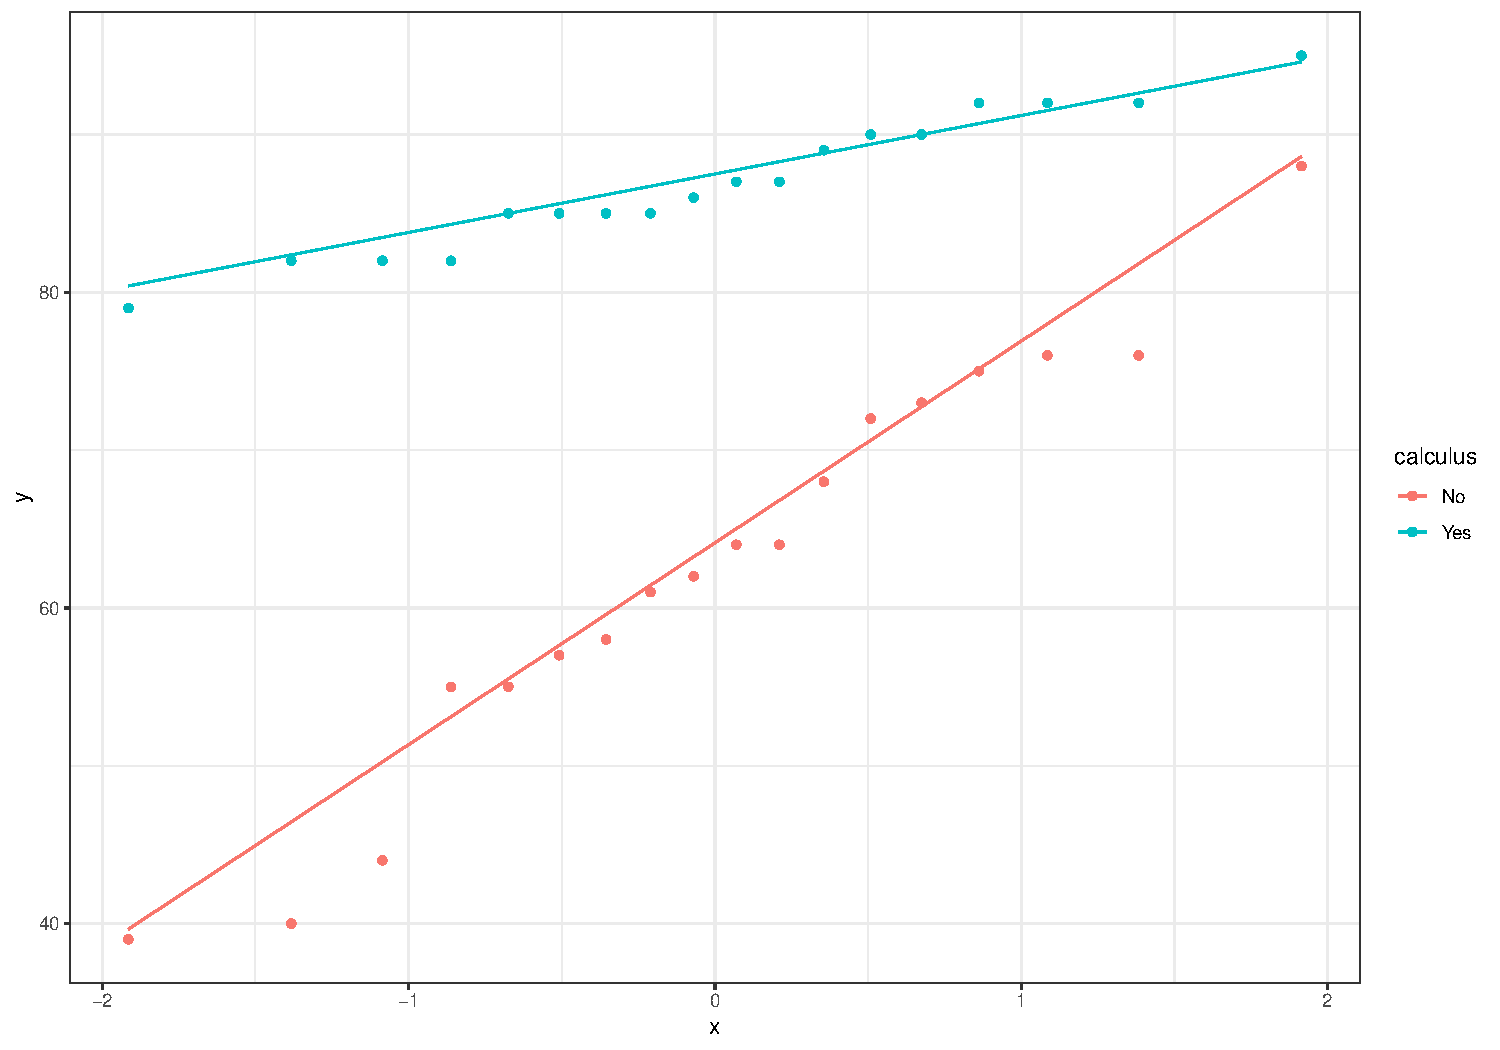
\includegraphics[width=0.7\linewidth,height=0.5\textheight]{Week11_12_13_files/figure-beamer/unnamed-chunk-2-1} \end{center}
\normalsize
\end{frame}

\begin{frame}[fragile]{Example 1}
\protect\hypertarget{example-1-2}{}
\small

\begin{Shaded}
\begin{Highlighting}[]
\NormalTok{CALCULUS }\SpecialCharTok{\%\textgreater{}\%} 
  \FunctionTok{group\_by}\NormalTok{(calculus) }\SpecialCharTok{\%\textgreater{}\%} 
  \FunctionTok{summarize}\NormalTok{(}\AttributeTok{Mean =} \FunctionTok{mean}\NormalTok{(score), }\AttributeTok{n =} \FunctionTok{n}\NormalTok{(), }\AttributeTok{SD =} \FunctionTok{sd}\NormalTok{(score))}
\end{Highlighting}
\end{Shaded}

\begin{verbatim}
# A tibble: 2 x 4
  calculus  Mean     n    SD
  <fct>    <dbl> <int> <dbl>
1 No        62.6    18 13.2 
2 Yes       86.9    18  4.32
\end{verbatim}

\normalsize

Because of the degrees of freedom, it is easier to use technology to get
the CI.
\end{frame}

\begin{frame}[fragile]{Example 1}
\protect\hypertarget{example-1-3}{}
\tiny

\begin{Shaded}
\begin{Highlighting}[]
\FunctionTok{t.test}\NormalTok{(score }\SpecialCharTok{\textasciitilde{}}\NormalTok{ calculus, }\AttributeTok{data =}\NormalTok{ CALCULUS, }\AttributeTok{conf.level =} \FloatTok{0.90}\NormalTok{)}
\end{Highlighting}
\end{Shaded}

\begin{verbatim}

    Welch Two Sample t-test

data:  score by calculus
t = -7.4219, df = 20.585, p-value = 3.04e-07
alternative hypothesis: true difference in means between group No and group Yes is not equal to 0
90 percent confidence interval:
 -29.98018 -18.68649
sample estimates:
 mean in group No mean in group Yes 
         62.61111          86.94444 
\end{verbatim}

\begin{Shaded}
\begin{Highlighting}[]
\FunctionTok{t.test}\NormalTok{(score }\SpecialCharTok{\textasciitilde{}}\NormalTok{ calculus, }\AttributeTok{data =}\NormalTok{ CALCULUS, }\AttributeTok{conf.level =} \FloatTok{0.90}\NormalTok{)}\SpecialCharTok{$}\NormalTok{conf.int }\OtherTok{{-}\textgreater{}}\NormalTok{ TTCI}
\NormalTok{TTCI}
\end{Highlighting}
\end{Shaded}

\begin{verbatim}
[1] -29.98018 -18.68649
attr(,"conf.level")
[1] 0.9
\end{verbatim}

\normalsize
\end{frame}

\begin{frame}[fragile]{Example 1}
\protect\hypertarget{example-1-4}{}
Compare to bootstrap CI: \tiny

\begin{Shaded}
\begin{Highlighting}[]
\FunctionTok{library}\NormalTok{(infer)}
\NormalTok{CI }\OtherTok{\textless{}{-}}\NormalTok{ CALCULUS }\SpecialCharTok{\%\textgreater{}\%} 
  \FunctionTok{specify}\NormalTok{(score }\SpecialCharTok{\textasciitilde{}}\NormalTok{ calculus) }\SpecialCharTok{\%\textgreater{}\%} 
  \FunctionTok{generate}\NormalTok{(}\AttributeTok{reps =} \DecValTok{1000}\NormalTok{, }\AttributeTok{type =} \StringTok{"bootstrap"}\NormalTok{) }\SpecialCharTok{\%\textgreater{}\%} 
  \FunctionTok{calculate}\NormalTok{(}\AttributeTok{stat =} \StringTok{"diff in means"}\NormalTok{, }\AttributeTok{order =} \FunctionTok{c}\NormalTok{(}\StringTok{"No"}\NormalTok{, }\StringTok{"Yes"}\NormalTok{))}
\FunctionTok{get\_ci}\NormalTok{(CI, }\AttributeTok{level =} \FloatTok{0.90}\NormalTok{)}
\end{Highlighting}
\end{Shaded}

\begin{verbatim}
# A tibble: 1 x 2
  lower_ci upper_ci
     <dbl>    <dbl>
1    -29.6    -18.9
\end{verbatim}

\begin{Shaded}
\begin{Highlighting}[]
\CommentTok{\# Compare to Theoretical T CI below}
\NormalTok{TTCI}
\end{Highlighting}
\end{Shaded}

\begin{verbatim}
[1] -29.98018 -18.68649
attr(,"conf.level")
[1] 0.9
\end{verbatim}

\normalsize
\end{frame}

\begin{frame}{Confidence Intervals for a Difference in Means}
\protect\hypertarget{confidence-intervals-for-a-difference-in-means-2}{}
\begin{itemize}
\item
  If the confidence interval for the difference in means contains 0,
  then we cannot rule out the possibility that the means might be the
  same, \(\mu_X-\mu_Y=0\) or, equivalently, \(\mu_X=\mu_Y\).
\item
  Skewness is less of an issue for the two-sample \(t\) confidence
  intervals than for one-sample intervals, because the skewness from the
  two samples tends to cancel out.

  \begin{itemize}
  \tightlist
  \item
    In particular, if the populations have the same skewness and
    variance and the sample sizes are equal, then the skewness cancels
    out exactly, and the distribution of \(t\) statistics can be very
    close to a \(t\) distribution even for quite small samples.
  \end{itemize}
\end{itemize}
\end{frame}

\begin{frame}[fragile]{Example 2}
\protect\hypertarget{example-2}{}
\begin{tcolorbox}
Consider the weights of boy and girl babies born in Texas in 2004. Construct a $95\%$ $t$ confidence interval for the mean difference in weights (boys -girls).
\end{tcolorbox}

We will use the \texttt{TXBirths2004} from the \texttt{resampledata}
package.
\end{frame}

\begin{frame}[fragile]{Example 2}
\protect\hypertarget{example-2-1}{}
\tiny

\begin{Shaded}
\begin{Highlighting}[]
\NormalTok{Texas }\OtherTok{\textless{}{-}}\NormalTok{ TXBirths2004}
\FunctionTok{ggplot}\NormalTok{(}\AttributeTok{data =}\NormalTok{ Texas, }\FunctionTok{aes}\NormalTok{(}\AttributeTok{x =}\NormalTok{ Weight)) }\SpecialCharTok{+} 
  \FunctionTok{geom\_histogram}\NormalTok{(}\AttributeTok{fill =} \StringTok{"blue"}\NormalTok{, }\AttributeTok{color =} \StringTok{"black"}\NormalTok{) }\SpecialCharTok{+} 
  \FunctionTok{facet\_grid}\NormalTok{(}\AttributeTok{rows =} \FunctionTok{vars}\NormalTok{(Gender)) }\SpecialCharTok{+} 
  \FunctionTok{theme\_bw}\NormalTok{()}
\end{Highlighting}
\end{Shaded}

\begin{center}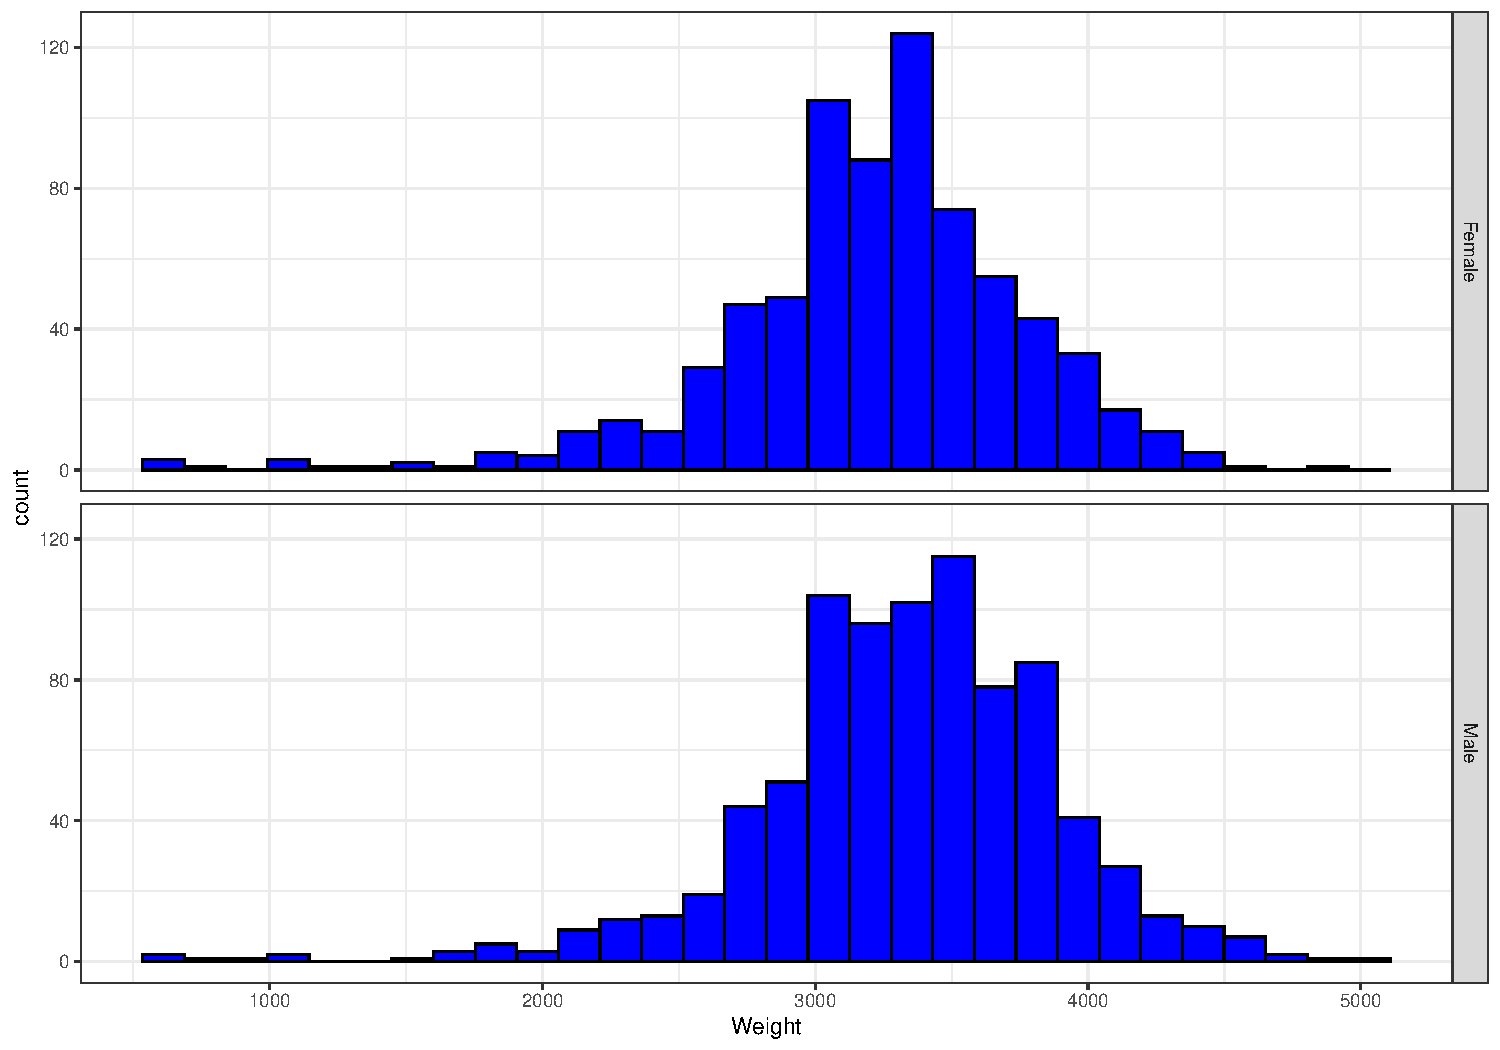
\includegraphics[width=0.7\linewidth,height=0.5\textheight]{Week11_12_13_files/figure-beamer/unnamed-chunk-6-1} \end{center}
\normalsize
\end{frame}

\begin{frame}[fragile]{Example 2}
\protect\hypertarget{example-2-2}{}
\tiny

\begin{Shaded}
\begin{Highlighting}[]
\FunctionTok{ggplot}\NormalTok{(}\AttributeTok{data =}\NormalTok{ Texas, }\FunctionTok{aes}\NormalTok{(}\AttributeTok{sample =}\NormalTok{ Weight)) }\SpecialCharTok{+} 
  \FunctionTok{stat\_qq}\NormalTok{(}\AttributeTok{color =} \FunctionTok{rgb}\NormalTok{(}\DecValTok{0}\NormalTok{, }\DecValTok{0}\NormalTok{, }\DecValTok{1}\NormalTok{, }\FloatTok{0.15}\NormalTok{)) }\SpecialCharTok{+} 
  \FunctionTok{facet\_grid}\NormalTok{(}\AttributeTok{rows =} \FunctionTok{vars}\NormalTok{(Gender)) }\SpecialCharTok{+} 
  \FunctionTok{theme\_bw}\NormalTok{()}
\end{Highlighting}
\end{Shaded}

\begin{center}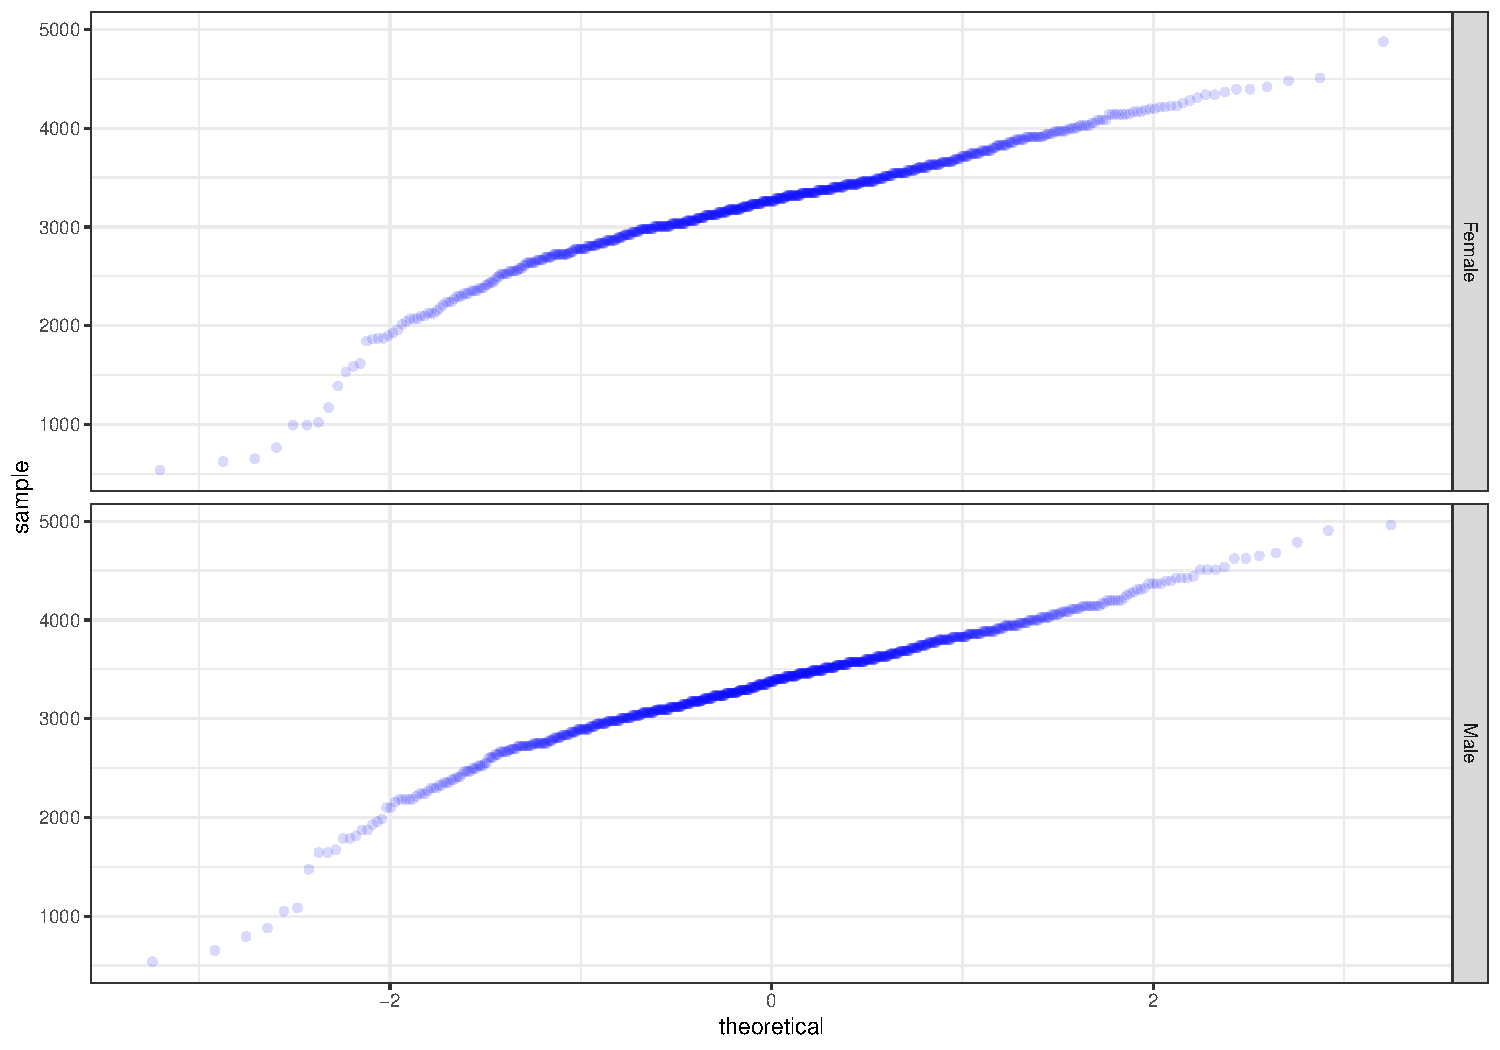
\includegraphics[width=0.8\linewidth,height=0.6\textheight]{Week11_12_13_files/figure-beamer/unnamed-chunk-7-1} \end{center}
\normalsize
\end{frame}

\begin{frame}[fragile]{Example 2}
\protect\hypertarget{example-2-3}{}
\tiny

\begin{Shaded}
\begin{Highlighting}[]
\FunctionTok{t.test}\NormalTok{(Weight }\SpecialCharTok{\textasciitilde{}}\NormalTok{ Gender, }\AttributeTok{data =}\NormalTok{ Texas)}
\end{Highlighting}
\end{Shaded}

\begin{verbatim}

    Welch Two Sample t-test

data:  Weight by Gender
t = -4.193, df = 1552.9, p-value = 2.908e-05
alternative hypothesis: true difference in means between group Female and group Male is not equal to 0
95 percent confidence interval:
 -170.12395  -61.68415
sample estimates:
mean in group Female   mean in group Male 
            3220.939             3336.843 
\end{verbatim}

\begin{Shaded}
\begin{Highlighting}[]
\NormalTok{Texas}\SpecialCharTok{$}\NormalTok{Gender }\OtherTok{\textless{}{-}} \FunctionTok{factor}\NormalTok{(Texas}\SpecialCharTok{$}\NormalTok{Gender, }\AttributeTok{levels =} \FunctionTok{c}\NormalTok{(}\StringTok{"Male"}\NormalTok{, }\StringTok{"Female"}\NormalTok{))}
\FunctionTok{t.test}\NormalTok{(Weight }\SpecialCharTok{\textasciitilde{}}\NormalTok{ Gender, }\AttributeTok{data =}\NormalTok{ Texas)}
\end{Highlighting}
\end{Shaded}

\begin{verbatim}

    Welch Two Sample t-test

data:  Weight by Gender
t = 4.193, df = 1552.9, p-value = 2.908e-05
alternative hypothesis: true difference in means between group Male and group Female is not equal to 0
95 percent confidence interval:
  61.68415 170.12395
sample estimates:
  mean in group Male mean in group Female 
            3336.843             3220.939 
\end{verbatim}

\normalsize
\end{frame}

\begin{frame}{Confidence Intervals for Proportions}
\protect\hypertarget{confidence-intervals-for-proportions}{}
\begin{tcolorbox}
In 2010, according to an AP-Gfk Poll conducted on October 13-18, $59\%$ of 846 likely voters responded that they felt things in this country were heading in the wrong direction (http:www.ap-gfkpoll.com/poll.archive.html). 
\end{tcolorbox}

\begin{itemize}
\item
  Let \(X\) denote the number of likely voters in a sample of size \(n\)
  who think the country is headed in the wrong direction.
\item
  We assume \(X\) is binomial, \(X\sim Bin(n, p)\).
\item
  We know that the proportion of likely voters, \(\hat{p}=\frac{X}{n}\)
  is an unbiased estimator of \(p\) and for large \(n\).
  \[Z=\frac{\hat{p}-p}{\sqrt{\frac{p(1-p)}{n}}}\] is approximately
  standard normal.
\end{itemize}
\end{frame}

\begin{frame}{Confidence Intervals for Proportions}
\protect\hypertarget{confidence-intervals-for-proportions-1}{}
Thus:
\[P\left(-z_{1-\alpha/2}<\frac{\hat{p}-p}{\sqrt{\frac{p(1-p)}{n}}}<z_{1-\alpha/2}\right)\approx 1-\alpha \]
This gives:
\[\frac{\hat{p}-p}{\sqrt{\frac{p(1-p)}{n}}}=\pm z_{1-\alpha/2}\]

At this point the different methods diverge.
\end{frame}

\begin{frame}{The Wald method}
\protect\hypertarget{the-wald-method}{}
The traditional Wald method completes the algebra to the following step
before making an approximation:

\[CI_{1 - \alpha}(p) = \hat{p}\pm z_{1-\alpha/2}\sqrt{\frac{p(1-p)}{n}}\]

At this point the Wald method replaces the population values \(p\) and
\(q\) in the right side of the equation with their approximations
\(\hat{p}\) and \(\hat{q}\) to obtain the traditional Wald confidence
interval formula for a proportion:
\[CI_{1 - \alpha}(p)=\hat{p}\pm z_{1-\alpha/2}\sqrt{\frac{\hat{p}(1-\hat{p})}{n}}\]
\end{frame}

\begin{frame}{The Wald method}
\protect\hypertarget{the-wald-method-1}{}
\begin{tcolorbox}
In 2010, according to an AP-Gfk Poll conducted on October 13-18, $59\%$ of 846 likely voters responded that they felt things in this country were heading in the wrong direction (http:www.ap-gfkpoll.com/poll.archive.html). Find a $95\%$ confidence interval. 
\end{tcolorbox}

\begin{tcolorbox}
For a $95\%$ confidence interval using $\hat{p}=0.59$, $n=846$ and $z_{1-\alpha/2}=1.96$ , we have
$$0.59\pm 1.96\sqrt{\frac{0.59(0.41)}{846}}=(0.5569,0.6231)$$
\end{tcolorbox}
\end{frame}

\begin{frame}[fragile]{The Wald method}
\protect\hypertarget{the-wald-method-2}{}
\small

\begin{Shaded}
\begin{Highlighting}[]
\NormalTok{x }\OtherTok{\textless{}{-}} \FloatTok{0.59}\SpecialCharTok{*}\DecValTok{846}
\NormalTok{n }\OtherTok{\textless{}{-}} \DecValTok{846}
\NormalTok{phat }\OtherTok{\textless{}{-}}\NormalTok{ x}\SpecialCharTok{/}\NormalTok{n}
\NormalTok{phat }\SpecialCharTok{+} \FunctionTok{c}\NormalTok{(}\SpecialCharTok{{-}}\DecValTok{1}\NormalTok{, }\DecValTok{1}\NormalTok{)}\SpecialCharTok{*}\FunctionTok{qnorm}\NormalTok{(.}\DecValTok{975}\NormalTok{)}\SpecialCharTok{*}\FunctionTok{sqrt}\NormalTok{(phat}\SpecialCharTok{*}\NormalTok{(}\DecValTok{1} \SpecialCharTok{{-}}\NormalTok{ phat)}\SpecialCharTok{/}\NormalTok{n)}
\end{Highlighting}
\end{Shaded}

\begin{verbatim}
[1] 0.5568578 0.6231422
\end{verbatim}

\begin{Shaded}
\begin{Highlighting}[]
\FunctionTok{library}\NormalTok{(binom)}
\FunctionTok{binom.confint}\NormalTok{(}\AttributeTok{x =}\NormalTok{ .}\DecValTok{59}\SpecialCharTok{*}\DecValTok{846}\NormalTok{, }\AttributeTok{n =} \DecValTok{846}\NormalTok{, }\AttributeTok{methods =} \StringTok{"asymptotic"}\NormalTok{)}
\end{Highlighting}
\end{Shaded}

\begin{verbatim}
      method      x   n mean     lower     upper
1 asymptotic 499.14 846 0.59 0.5568578 0.6231422
\end{verbatim}

\normalsize
\end{frame}

\begin{frame}{The Agresti-Coull Interval for a Proportion}
\protect\hypertarget{the-agresti-coull-interval-for-a-proportion}{}
Agresti and Coull (1998) considered the \(95\%\) confidence interval for
which the 0.975 quantile is \(z_{0.975}\approx1.96\), and hence
\(z^2_{0.975}\approx 4\)

\begin{itemize}
\tightlist
\item
  If \(X\) denotes the number of successes in a sample of size \(n\),
  let \(\tilde{X}=X+2\), \(\tilde{n}=n+4\), and
  \(\tilde{p}=\frac{\tilde{X}}{\tilde{n}}\).
\end{itemize}

Then the \((1-\alpha)\times 100\) confidence interval is given by:
\[CI_{1 - \alpha}(p) = \tilde{p}\pm z_{1-\alpha/2}\sqrt{\frac{\tilde{p}(1-\tilde{p})}{\tilde{n}}}\]
\end{frame}

\begin{frame}{The Agresti-Coull Interval for a Proportion}
\protect\hypertarget{the-agresti-coull-interval-for-a-proportion-1}{}
\begin{tcolorbox}
In 2010, according to an AP-Gfk Poll conducted on October 13-18, $59\%$ of 846 likely voters responded that they felt things in this country were heading in the wrong direction (http:www.ap-gfkpoll.com/poll.archive.html). Find a $95\%$ confidence interval. 
\end{tcolorbox}

\begin{tcolorbox}
For a $95\%$ confidence interval using $\hat{p}=0.59$, $n=846$ and $z_{1-\alpha/2}=1.96$ , we have $\tilde{X}=0.59(846)+2=501.14$, $\tilde{n}=846+4=850$ and $\tilde{p}=0.5896$
$$CI_{1 - \alpha}(p)=0.5896\pm 1.96\sqrt{\frac{0.5896(0.4104)}{850}}=(0.5565,0.6226)$$
\end{tcolorbox}
\end{frame}

\begin{frame}[fragile]{The Agresti-Coull Interval for a Proportion}
\protect\hypertarget{the-agresti-coull-interval-for-a-proportion-2}{}
\small

\begin{Shaded}
\begin{Highlighting}[]
\NormalTok{xtilde }\OtherTok{\textless{}{-}} \FloatTok{0.59}\SpecialCharTok{*}\DecValTok{846} \SpecialCharTok{+} \DecValTok{2}
\NormalTok{ntilde }\OtherTok{\textless{}{-}} \DecValTok{846} \SpecialCharTok{+} \DecValTok{4}
\NormalTok{ptilde }\OtherTok{\textless{}{-}}\NormalTok{ xtilde}\SpecialCharTok{/}\NormalTok{ntilde}
\NormalTok{ptilde }\SpecialCharTok{+} \FunctionTok{c}\NormalTok{(}\SpecialCharTok{{-}}\DecValTok{1}\NormalTok{, }\DecValTok{1}\NormalTok{)}\SpecialCharTok{*}\FunctionTok{qnorm}\NormalTok{(.}\DecValTok{975}\NormalTok{)}\SpecialCharTok{*}\FunctionTok{sqrt}\NormalTok{(ptilde}\SpecialCharTok{*}\NormalTok{(}\DecValTok{1} \SpecialCharTok{{-}}\NormalTok{ ptilde)}\SpecialCharTok{/}\NormalTok{ntilde)}
\end{Highlighting}
\end{Shaded}

\begin{verbatim}
[1] 0.5565072 0.6226458
\end{verbatim}

\begin{Shaded}
\begin{Highlighting}[]
\CommentTok{\# Or}
\FunctionTok{binom.confint}\NormalTok{(}\AttributeTok{x =}\NormalTok{ .}\DecValTok{59}\SpecialCharTok{*}\DecValTok{846}\NormalTok{, }\AttributeTok{n =} \DecValTok{846}\NormalTok{, }\AttributeTok{methods =} \StringTok{"ac"}\NormalTok{)}
\end{Highlighting}
\end{Shaded}

\begin{verbatim}
         method      x   n mean    lower     upper
1 agresti-coull 499.14 846 0.59 0.556521 0.6226653
\end{verbatim}

\normalsize
\end{frame}

\begin{frame}{Wilson Score method}
\protect\hypertarget{wilson-score-method}{}
The Wilson Score method does not make the approximation to the equation
below
\[CI_{1 - \alpha}(p)=\hat{p}\pm z_{1-\alpha/2}\sqrt{\frac{p(1-p)}{n}}\]

The result is more involved algebra (which involves solving a quadratic
equation), and a more complicated solution.

\begin{itemize}
\tightlist
\item
  The result is the Wilson Score confidence interval for a proportion:
  \[CI_{1-\alpha}(p)=\frac{\hat{p}+\frac{z^2_{1-\alpha/2}}{2n}\pm z_{1-\alpha/2}\sqrt{\frac{\hat{p}(1-\hat{p})}{n}+\frac{z^2_{1-\alpha/2}}{4n^2}}}{1+\frac{z^2_{1-\alpha/2}}{n}}\]
\end{itemize}
\end{frame}

\begin{frame}{Wilson Score method}
\protect\hypertarget{wilson-score-method-1}{}
\begin{tcolorbox}
In 2010, according to an AP-Gfk Poll conducted on October 13-18, $59\%$ of 846 likely voters responded that they felt things in this country were heading in the wrong direction (http:www.ap-gfkpoll.com/poll.archive.html). Find a $95\%$ confidence interval. 
\end{tcolorbox}

\begin{tcolorbox}
For a $95\%$ confidence interval using $\hat{p}=0.59$, and $n=846$ we have:
$$p=\frac{0.59+\frac{1.96^2}{2(846)}\pm 1.96\sqrt{\frac{0.59(0.41)}{846}+\frac{1.96^2}{4(846^2)}}}{1+\frac{1.96^2}{846}}=(0.5565,0.6227)$$
\end{tcolorbox}
\end{frame}

\begin{frame}[fragile]{Wilson Score method}
\protect\hypertarget{wilson-score-method-2}{}
\tiny

\begin{Shaded}
\begin{Highlighting}[]
\FunctionTok{prop.test}\NormalTok{(}\AttributeTok{x =} \FloatTok{499.14}\NormalTok{, }\AttributeTok{n =} \DecValTok{846}\NormalTok{, }\AttributeTok{conf.level =} \FloatTok{0.95}\NormalTok{, }\AttributeTok{correct =} \ConstantTok{FALSE}\NormalTok{)}
\end{Highlighting}
\end{Shaded}

\begin{verbatim}

    1-sample proportions test without continuity correction

data:  499.14 out of 846, null probability 0.5
X-squared = 27.41, df = 1, p-value = 1.645e-07
alternative hypothesis: true p is not equal to 0.5
95 percent confidence interval:
 0.5565235 0.6226629
sample estimates:
   p 
0.59 
\end{verbatim}

\begin{Shaded}
\begin{Highlighting}[]
\CommentTok{\# Or}
\FunctionTok{binom.confint}\NormalTok{(}\AttributeTok{x =}\NormalTok{ .}\DecValTok{59}\SpecialCharTok{*}\DecValTok{846}\NormalTok{, }\AttributeTok{n =} \DecValTok{846}\NormalTok{, }\AttributeTok{methods =} \StringTok{"wilson"}\NormalTok{)}
\end{Highlighting}
\end{Shaded}

\begin{verbatim}
  method      x   n mean     lower     upper
1 wilson 499.14 846 0.59 0.5565235 0.6226629
\end{verbatim}

\normalsize
\end{frame}

\begin{frame}{Example}
\protect\hypertarget{example}{}
\begin{tcolorbox}
A political candidate prepares to conduct a survey to gauge voter support for his candidacy for senator. He would like a confidence interval with an error of at most $4\%$, with $95\%$ confidence. How large should the sample size be for the survey? 
\end{tcolorbox}

\begin{tcolorbox}
Solution:  Since the Agresti-Coull interval is symmetric, the margin of error is $1.96\sqrt{\frac{\tilde{p}(1-\tilde{p})}{\tilde{n}}}$. Thus, we want to solve for $\tilde{n}$ in $$1.96\sqrt{\frac{\tilde{p}(1-\tilde{p})}{\tilde{n}}}\leq 0.04$$
Unfortunately, we do not know $\tilde{p}$. If we did, the candidate would not need to conduct the survey! We will use $\tilde{p}=0.5$ since this will maximize the expression under the radical sign. 

\end{tcolorbox}
\end{frame}

\begin{frame}[fragile]{Example}
\protect\hypertarget{example-3}{}
\tiny

\begin{Shaded}
\begin{Highlighting}[]
\NormalTok{ptilde }\OtherTok{\textless{}{-}} \FunctionTok{seq}\NormalTok{(}\DecValTok{0}\NormalTok{, }\DecValTok{1}\NormalTok{, }\AttributeTok{length =} \DecValTok{1000}\NormalTok{)}
\NormalTok{fptilde }\OtherTok{\textless{}{-}} \FunctionTok{sqrt}\NormalTok{(ptilde}\SpecialCharTok{*}\NormalTok{(}\DecValTok{1} \SpecialCharTok{{-}}\NormalTok{ ptilde))}
\FunctionTok{plot}\NormalTok{(ptilde, fptilde, }\AttributeTok{type =} \StringTok{"l"}\NormalTok{, }\AttributeTok{ylab =} \StringTok{""}\NormalTok{, }\AttributeTok{xlab =}\FunctionTok{expression}\NormalTok{(}\FunctionTok{tilde}\NormalTok{(p)))}
\end{Highlighting}
\end{Shaded}

\begin{center}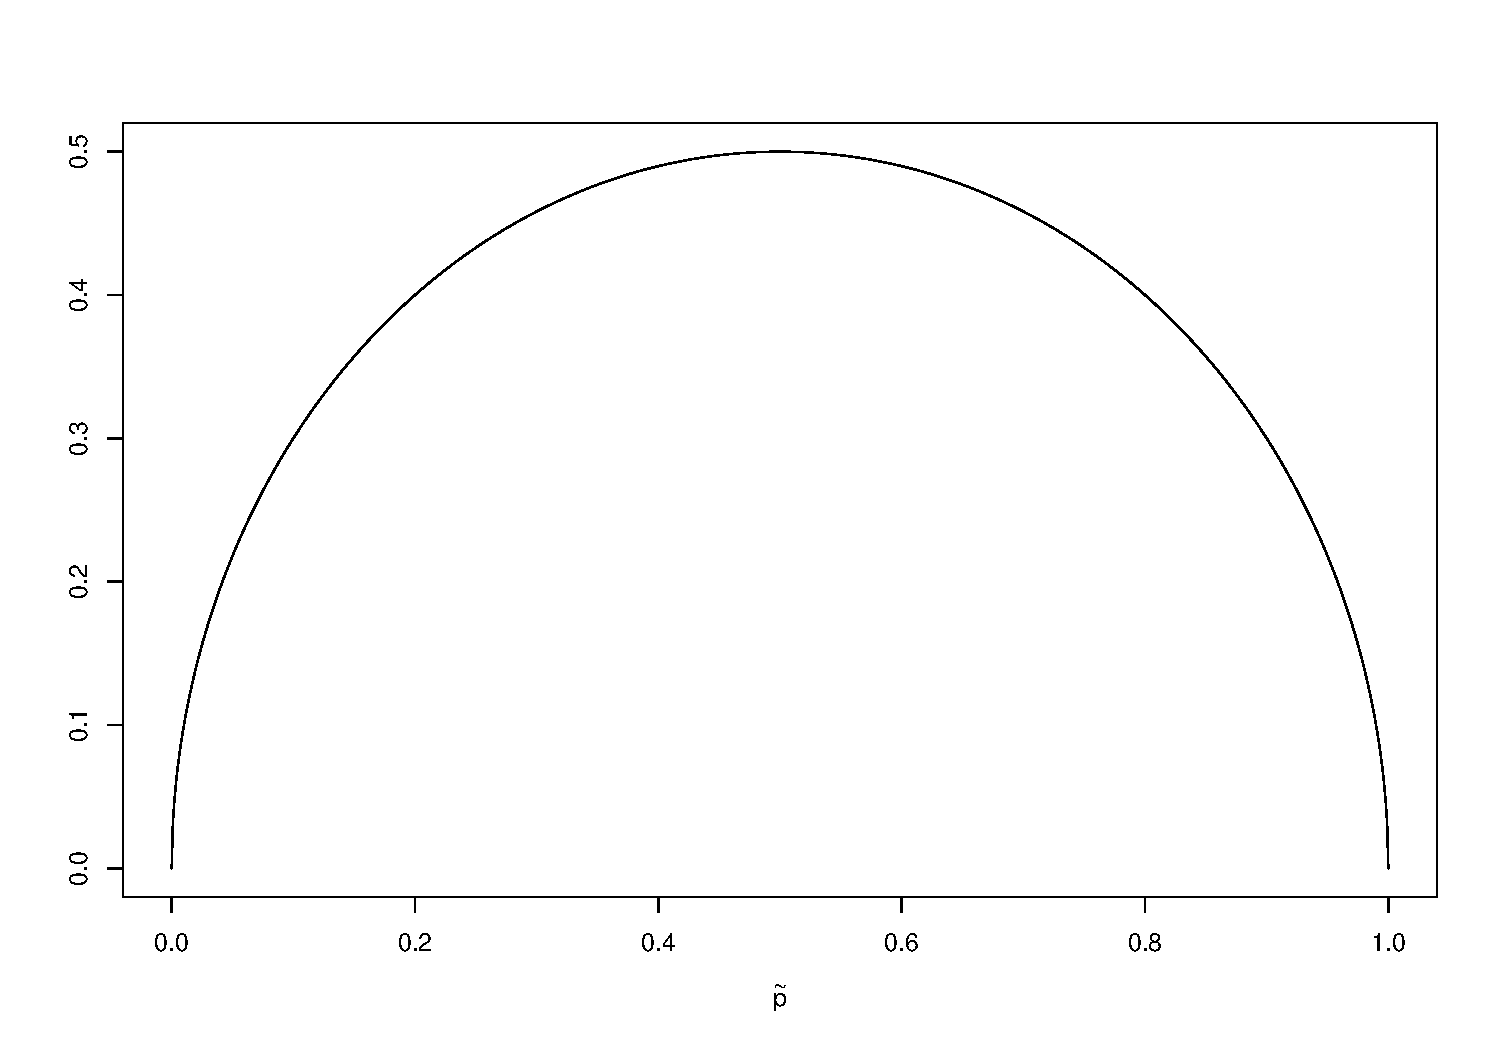
\includegraphics[width=0.6\linewidth,height=0.4\textheight]{Week11_12_13_files/figure-beamer/unnamed-chunk-12-1} \end{center}
\normalsize

\[1.96\sqrt{\frac{0.5(1-0.5)}{\tilde{n}}}\leq 0.04\]
\end{frame}

\begin{frame}[fragile]{Example}
\protect\hypertarget{example-4}{}
Solving for \(\tilde{n}\) yields
\[\left(\frac{1.96(0.5)}{0.04}\right)^2\leq \tilde{n} \implies \tilde{n}\geq 600.25\]

Then \[n\geq 596.25\] \tiny

\begin{Shaded}
\begin{Highlighting}[]
\NormalTok{ntilde }\OtherTok{\textless{}{-}}\NormalTok{ (}\FloatTok{1.96}\SpecialCharTok{*}\NormalTok{(}\FloatTok{0.5}\NormalTok{)}\SpecialCharTok{/}\FloatTok{0.04}\NormalTok{)}\SpecialCharTok{\^{}}\DecValTok{2}
\NormalTok{n }\OtherTok{\textless{}{-}}\NormalTok{ ntilde }\SpecialCharTok{{-}} \DecValTok{4}
\NormalTok{n }\OtherTok{\textless{}{-}} \FunctionTok{ceiling}\NormalTok{(n)}
\NormalTok{n}
\end{Highlighting}
\end{Shaded}

\begin{verbatim}
[1] 597
\end{verbatim}

\normalsize
\end{frame}

\begin{frame}{Coverage Probabilities of Binomial Confidence Intervals}
\protect\hypertarget{coverage-probabilities-of-binomial-confidence-intervals}{}
\begin{itemize}
\item
  Suppose a new process for making a prescription drug is in
  development.

  \begin{itemize}
  \tightlist
  \item
    Of \(n=30\) trial batches made with the current version of the
    process,
  \item
    \(X=24\) batches give satisfactory results.
  \item
    Then \(\hat{p}=24/30=0.8\) estimates the population proportion
    \(p=P(Success)\) of satisfactory batches with the current version of
    the process.
  \end{itemize}
\item
  Wondering how near \(\hat{p}\) might be to \(p\), the investigators
  use the Wald CI method:
  \[CI_{1 - \alpha}(p) =\hat{p}\pm z_{1-\alpha/2}\sqrt{\frac{\hat{p}(1-\hat{p})}{n}}\]
\end{itemize}

to obtain the approximate \(95\%\) confidence interval
\(0.8 \pm 0.1431355\) or \((0.6568645, 0.9431355)\)
\end{frame}

\begin{frame}{Coverage Probabilities of Binomial Confidence Intervals}
\protect\hypertarget{coverage-probabilities-of-binomial-confidence-intervals-1}{}
The question is whether a \(95\%\) level of confidence in the resulting
interval is warranted.

\begin{itemize}
\item
  If the Wald CI method is used repeatedly, in what proportion of
  instances does it yield an interval that covers the true value \(p\)?

  \begin{itemize}
  \tightlist
  \item
    If Wald CI method is valid here, then the simple answer ought to be
    \(95\%\).
  \item
    Unfortunately, there is no simple answer to this question. It turns
    out that the coverage probability depends on the value of \(p\).
  \end{itemize}
\end{itemize}
\end{frame}

\begin{frame}{Coverage Probabilities of Binomial Confidence Intervals}
\protect\hypertarget{coverage-probabilities-of-binomial-confidence-intervals-2}{}
\begin{itemize}
\item
  Now choose a particular value of \(p\), say \(p=0.8\), so that

  \begin{itemize}
  \tightlist
  \item
    \(X\) has a binomial distribution with \(n=30\) trials and
    probability of success \((p=0.8)\).
  \item
    \(X\sim Bin(n=30, p=0.8)\).
  \item
    The vector of prob of the 31 probabilities \(P(X=x)\),
    \(X=0, 1, \ldots, 30\) in this distribution is found.
  \end{itemize}
\item
  Next, we determine which of the 31 confidence intervals cover the
  value \(p=0.8\).

  \begin{itemize}
  \tightlist
  \item
    Finally, the coverage probability is computed: It is the sum of the
    probabilities corresponding to values of \(x\) that yield intervals
    covering \(p\).
  \end{itemize}
\end{itemize}
\end{frame}

\begin{frame}[fragile]{Coverage Probabilities of Binomial Confidence
Intervals}
\protect\hypertarget{coverage-probabilities-of-binomial-confidence-intervals-3}{}
\tiny

\begin{Shaded}
\begin{Highlighting}[]
\NormalTok{alpha }\OtherTok{\textless{}{-}} \FloatTok{0.05}
\NormalTok{n }\OtherTok{\textless{}{-}} \DecValTok{30}   \CommentTok{\# number of trials}
\NormalTok{x }\OtherTok{\textless{}{-}} \DecValTok{0}\SpecialCharTok{:}\NormalTok{n  }
\NormalTok{sp }\OtherTok{\textless{}{-}}\NormalTok{ x}\SpecialCharTok{/}\NormalTok{n }\CommentTok{\# sample proportion}
\NormalTok{m.err }\OtherTok{\textless{}{-}} \FunctionTok{qnorm}\NormalTok{(}\DecValTok{1} \SpecialCharTok{{-}}\NormalTok{ alpha}\SpecialCharTok{/}\DecValTok{2}\NormalTok{)}\SpecialCharTok{*}\FunctionTok{sqrt}\NormalTok{(sp}\SpecialCharTok{*}\NormalTok{(}\DecValTok{1} \SpecialCharTok{{-}}\NormalTok{ sp)}\SpecialCharTok{/}\NormalTok{n)}
\NormalTok{lcl }\OtherTok{\textless{}{-}}\NormalTok{ sp }\SpecialCharTok{{-}}\NormalTok{ m.err}
\NormalTok{ucl }\OtherTok{\textless{}{-}}\NormalTok{ sp }\SpecialCharTok{+}\NormalTok{ m.err}
\NormalTok{pp }\OtherTok{\textless{}{-}} \FloatTok{0.8}   \CommentTok{\# pp = P(Success)}
\NormalTok{prob }\OtherTok{\textless{}{-}} \FunctionTok{dbinom}\NormalTok{(x, n, pp)}
\NormalTok{cover }\OtherTok{\textless{}{-}}\NormalTok{ (pp }\SpecialCharTok{\textgreater{}=}\NormalTok{ lcl) }\SpecialCharTok{\&}\NormalTok{ (pp }\SpecialCharTok{\textless{}=}\NormalTok{ ucl)  }\CommentTok{\# vector of 0s and 1s}
\NormalTok{RES }\OtherTok{\textless{}{-}} \FunctionTok{round}\NormalTok{(}\FunctionTok{cbind}\NormalTok{(x, sp, lcl, ucl, prob, cover), }\DecValTok{4}\NormalTok{)}
\NormalTok{RES[}\DecValTok{19}\SpecialCharTok{:}\DecValTok{30}\NormalTok{, ]}
\end{Highlighting}
\end{Shaded}

\begin{verbatim}
       x     sp    lcl    ucl   prob cover
 [1,] 18 0.6000 0.4247 0.7753 0.0064     0
 [2,] 19 0.6333 0.4609 0.8058 0.0161     1
 [3,] 20 0.6667 0.4980 0.8354 0.0355     1
 [4,] 21 0.7000 0.5360 0.8640 0.0676     1
 [5,] 22 0.7333 0.5751 0.8916 0.1106     1
 [6,] 23 0.7667 0.6153 0.9180 0.1538     1
 [7,] 24 0.8000 0.6569 0.9431 0.1795     1
 [8,] 25 0.8333 0.7000 0.9667 0.1723     1
 [9,] 26 0.8667 0.7450 0.9883 0.1325     1
[10,] 27 0.9000 0.7926 1.0074 0.0785     1
[11,] 28 0.9333 0.8441 1.0226 0.0337     0
[12,] 29 0.9667 0.9024 1.0309 0.0093     0
\end{verbatim}

\begin{Shaded}
\begin{Highlighting}[]
\FunctionTok{sum}\NormalTok{(}\FunctionTok{dbinom}\NormalTok{(x[cover], n, pp))  }\CommentTok{\# total coverage prob at pp}
\end{Highlighting}
\end{Shaded}

\begin{verbatim}
[1] 0.9463279
\end{verbatim}

\normalsize
\end{frame}

\begin{frame}[fragile]{Coverage Probabilities of Binomial Confidence
Intervals}
\protect\hypertarget{coverage-probabilities-of-binomial-confidence-intervals-4}{}
Now use \(p=0.79\) \tiny

\begin{Shaded}
\begin{Highlighting}[]
\NormalTok{alpha }\OtherTok{\textless{}{-}} \FloatTok{0.05}
\NormalTok{n }\OtherTok{\textless{}{-}} \DecValTok{30}   \CommentTok{\# number of trials}
\NormalTok{x }\OtherTok{\textless{}{-}} \DecValTok{0}\SpecialCharTok{:}\NormalTok{n  }
\NormalTok{sp }\OtherTok{\textless{}{-}}\NormalTok{ x}\SpecialCharTok{/}\NormalTok{n }\CommentTok{\# sample proportion}
\NormalTok{m.err }\OtherTok{\textless{}{-}} \FunctionTok{qnorm}\NormalTok{(}\DecValTok{1} \SpecialCharTok{{-}}\NormalTok{ alpha}\SpecialCharTok{/}\DecValTok{2}\NormalTok{)}\SpecialCharTok{*}\FunctionTok{sqrt}\NormalTok{(sp}\SpecialCharTok{*}\NormalTok{(}\DecValTok{1} \SpecialCharTok{{-}}\NormalTok{ sp)}\SpecialCharTok{/}\NormalTok{n)}
\NormalTok{lcl }\OtherTok{\textless{}{-}}\NormalTok{ sp }\SpecialCharTok{{-}}\NormalTok{ m.err}
\NormalTok{ucl }\OtherTok{\textless{}{-}}\NormalTok{ sp }\SpecialCharTok{+}\NormalTok{ m.err}
\NormalTok{pp }\OtherTok{\textless{}{-}} \FloatTok{0.79}   \CommentTok{\# pp = P(Success)}
\NormalTok{prob }\OtherTok{\textless{}{-}} \FunctionTok{dbinom}\NormalTok{(x, n, pp)}
\NormalTok{cover }\OtherTok{\textless{}{-}}\NormalTok{ (pp }\SpecialCharTok{\textgreater{}=}\NormalTok{ lcl) }\SpecialCharTok{\&}\NormalTok{ (pp }\SpecialCharTok{\textless{}=}\NormalTok{ ucl)  }\CommentTok{\# vector of 0s and 1s}
\NormalTok{RES }\OtherTok{\textless{}{-}} \FunctionTok{round}\NormalTok{(}\FunctionTok{cbind}\NormalTok{(x, sp, lcl, ucl, prob, cover), }\DecValTok{4}\NormalTok{)}
\CommentTok{\#RES[18:31, ]}
\FunctionTok{sum}\NormalTok{(}\FunctionTok{dbinom}\NormalTok{(x[cover], n, pp))  }\CommentTok{\# total coverage prob at pp}
\end{Highlighting}
\end{Shaded}

\begin{verbatim}
[1] 0.8875662
\end{verbatim}

\normalsize
\end{frame}

\begin{frame}[fragile]{Coverage Probabilities of Binomial Confidence
Intervals - Wald}
\protect\hypertarget{coverage-probabilities-of-binomial-confidence-intervals---wald}{}
We step through two thousand values of \(p\) from near 0 to near 1.
Subsequently plot coverage probability versus \(p\).

\tiny

\begin{Shaded}
\begin{Highlighting}[]
\FunctionTok{par}\NormalTok{(}\AttributeTok{mfrow=}\FunctionTok{c}\NormalTok{(}\DecValTok{2}\NormalTok{, }\DecValTok{2}\NormalTok{))}
\ControlFlowTok{for}\NormalTok{(alpha }\ControlFlowTok{in} \FunctionTok{c}\NormalTok{(}\FloatTok{0.01}\NormalTok{, }\FloatTok{0.02}\NormalTok{, }\FloatTok{0.05}\NormalTok{, }\FloatTok{0.10}\NormalTok{))\{}
\NormalTok{n }\OtherTok{\textless{}{-}} \DecValTok{30}     \CommentTok{\# number of trials}
\NormalTok{CL }\OtherTok{\textless{}{-}} \DecValTok{1} \SpecialCharTok{{-}}\NormalTok{ alpha}
\NormalTok{x }\OtherTok{\textless{}{-}} \DecValTok{0}\SpecialCharTok{:}\NormalTok{n }
\NormalTok{adj }\OtherTok{\textless{}{-}} \DecValTok{0}    \CommentTok{\#(2 for Agresti{-}Coull)}
\NormalTok{k }\OtherTok{\textless{}{-}} \FunctionTok{qnorm}\NormalTok{(}\DecValTok{1} \SpecialCharTok{{-}}\NormalTok{ alpha}\SpecialCharTok{/}\DecValTok{2}\NormalTok{)}
\NormalTok{sp }\OtherTok{\textless{}{-}}\NormalTok{ (x }\SpecialCharTok{+}\NormalTok{ adj)}\SpecialCharTok{/}\NormalTok{(n }\SpecialCharTok{+} \DecValTok{2}\SpecialCharTok{*}\NormalTok{adj)}
\NormalTok{m.err }\OtherTok{\textless{}{-}}\NormalTok{ k }\SpecialCharTok{*} \FunctionTok{sqrt}\NormalTok{(sp}\SpecialCharTok{*}\NormalTok{(}\DecValTok{1} \SpecialCharTok{{-}}\NormalTok{ sp)}\SpecialCharTok{/}\NormalTok{(n }\SpecialCharTok{+} \DecValTok{2}\SpecialCharTok{*}\NormalTok{adj))}
\NormalTok{lcl }\OtherTok{\textless{}{-}}\NormalTok{ sp }\SpecialCharTok{{-}}\NormalTok{ m.err}
\NormalTok{ucl }\OtherTok{\textless{}{-}}\NormalTok{ sp }\SpecialCharTok{+}\NormalTok{ m.err}
\NormalTok{m }\OtherTok{\textless{}{-}} \DecValTok{2000} \CommentTok{\# number of values of pp}
\NormalTok{pp }\OtherTok{\textless{}{-}} \FunctionTok{seq}\NormalTok{(}\DecValTok{1}\SpecialCharTok{/}\NormalTok{n, }\DecValTok{1} \SpecialCharTok{{-}} \DecValTok{1}\SpecialCharTok{/}\NormalTok{n, }\AttributeTok{length =}\NormalTok{ m)}
\NormalTok{p.cov }\OtherTok{\textless{}{-}} \FunctionTok{numeric}\NormalTok{(m)}
\ControlFlowTok{for}\NormalTok{(i }\ControlFlowTok{in} \DecValTok{1}\SpecialCharTok{:}\NormalTok{m)\{}
\NormalTok{  cover }\OtherTok{\textless{}{-}}\NormalTok{ (pp[i] }\SpecialCharTok{\textgreater{}=}\NormalTok{ lcl) }\SpecialCharTok{\&}\NormalTok{ (pp[i] }\SpecialCharTok{\textless{}=}\NormalTok{ ucl)  }\CommentTok{\# vector of 0s and 1s}
\NormalTok{  p.rel }\OtherTok{\textless{}{-}} \FunctionTok{dbinom}\NormalTok{(x[cover], n, pp[i])}
\NormalTok{  p.cov[i] }\OtherTok{\textless{}{-}} \FunctionTok{sum}\NormalTok{(p.rel)}
\NormalTok{\}}
\FunctionTok{plot}\NormalTok{(pp, p.cov, }\AttributeTok{type =} \StringTok{"l"}\NormalTok{, }\AttributeTok{ylim =}\FunctionTok{c}\NormalTok{(}\FloatTok{0.60}\NormalTok{, }\FloatTok{1.1}\NormalTok{), }\AttributeTok{main =} \FunctionTok{paste}\NormalTok{(}\StringTok{"n = "}\NormalTok{, n), }
     \AttributeTok{xlab =} \StringTok{"p"}\NormalTok{, }\AttributeTok{ylab =} \StringTok{"Coverage Probability"}\NormalTok{)}
\FunctionTok{lines}\NormalTok{(}\FunctionTok{c}\NormalTok{(}\DecValTok{1}\SpecialCharTok{/}\NormalTok{n, }\DecValTok{1}\SpecialCharTok{{-}} \DecValTok{1}\SpecialCharTok{/}\NormalTok{n), }\FunctionTok{c}\NormalTok{(}\DecValTok{1} \SpecialCharTok{{-}}\NormalTok{ alpha, }\DecValTok{1}\SpecialCharTok{{-}}\NormalTok{ alpha), }\AttributeTok{col =} \StringTok{"red"}\NormalTok{, }\AttributeTok{lty =} \StringTok{"dashed"}\NormalTok{)}
      \FunctionTok{text}\NormalTok{(}\FloatTok{0.5}\NormalTok{, CL }\SpecialCharTok{+} \FloatTok{0.05}\NormalTok{, }\FunctionTok{paste}\NormalTok{(}\StringTok{"Targeted Confidence Level ="}\NormalTok{, CL))}
\NormalTok{\}}
\end{Highlighting}
\end{Shaded}

\normalsize
\end{frame}

\begin{frame}{Coverage Probabilities of Binomial Confidence Intervals -
Wald}
\protect\hypertarget{coverage-probabilities-of-binomial-confidence-intervals---wald-1}{}
\tiny

\begin{center}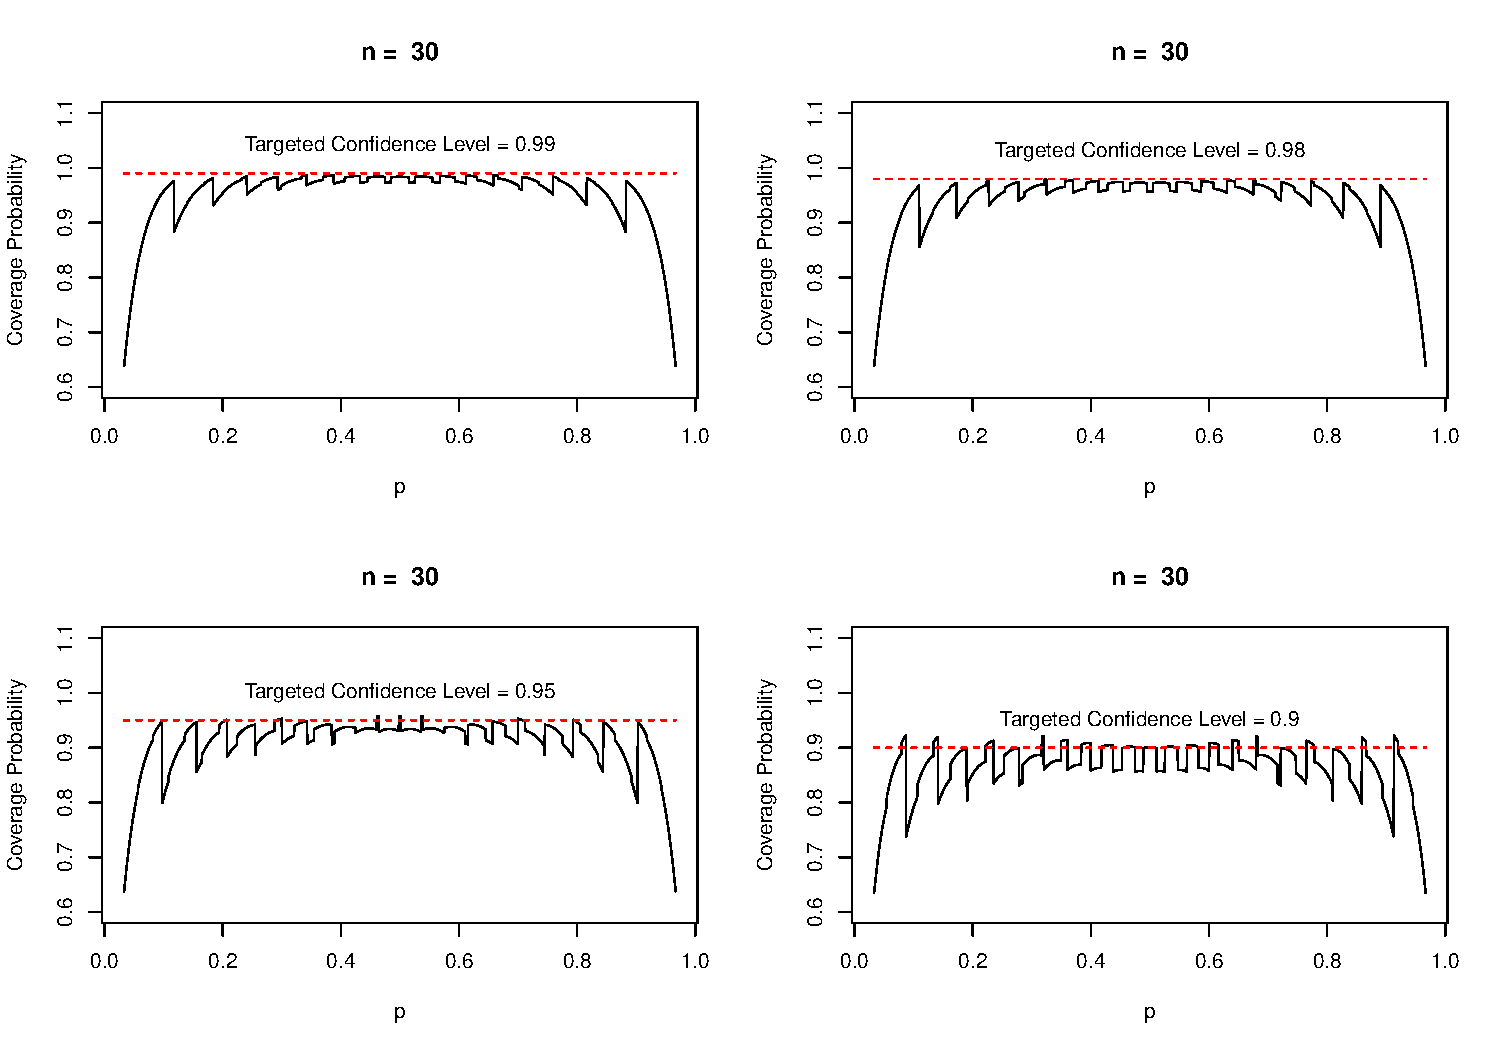
\includegraphics[width=0.9\linewidth,height=0.8\textheight]{Week11_12_13_files/figure-beamer/unnamed-chunk-17-1} \end{center}
\normalsize
\end{frame}

\begin{frame}[fragile]{Coverage Probabilities of Binomial Confidence
Intervals - Agresti-Coull}
\protect\hypertarget{coverage-probabilities-of-binomial-confidence-intervals---agresti-coull}{}
Next consider the Agresti-Coull confidence intervals.

\tiny

\begin{Shaded}
\begin{Highlighting}[]
\FunctionTok{par}\NormalTok{(}\AttributeTok{mfrow=}\FunctionTok{c}\NormalTok{(}\DecValTok{2}\NormalTok{, }\DecValTok{2}\NormalTok{))}
\ControlFlowTok{for}\NormalTok{(alpha }\ControlFlowTok{in} \FunctionTok{c}\NormalTok{(}\FloatTok{0.01}\NormalTok{, }\FloatTok{0.02}\NormalTok{, }\FloatTok{0.05}\NormalTok{, }\FloatTok{0.10}\NormalTok{))\{}
\NormalTok{n }\OtherTok{\textless{}{-}} \DecValTok{30}     \CommentTok{\# number of trials}
\NormalTok{CL }\OtherTok{\textless{}{-}} \DecValTok{1} \SpecialCharTok{{-}}\NormalTok{ alpha}
\NormalTok{x }\OtherTok{\textless{}{-}} \DecValTok{0}\SpecialCharTok{:}\NormalTok{n }
\NormalTok{adj }\OtherTok{\textless{}{-}} \DecValTok{2}  \CommentTok{\# 0 for large sample 2 for Agresti Coull}
\NormalTok{z }\OtherTok{\textless{}{-}} \FunctionTok{qnorm}\NormalTok{(}\DecValTok{1} \SpecialCharTok{{-}}\NormalTok{ alpha}\SpecialCharTok{/}\DecValTok{2}\NormalTok{)}
\NormalTok{sp }\OtherTok{\textless{}{-}}\NormalTok{ (x }\SpecialCharTok{+}\NormalTok{ adj)}\SpecialCharTok{/}\NormalTok{(n }\SpecialCharTok{+} \DecValTok{2}\SpecialCharTok{*}\NormalTok{adj)}
\NormalTok{m.err }\OtherTok{\textless{}{-}}\NormalTok{ z}\SpecialCharTok{*}\FunctionTok{sqrt}\NormalTok{(sp}\SpecialCharTok{*}\NormalTok{(}\DecValTok{1} \SpecialCharTok{{-}}\NormalTok{ sp)}\SpecialCharTok{/}\NormalTok{(n }\SpecialCharTok{+} \DecValTok{2}\SpecialCharTok{*}\NormalTok{adj))}
\NormalTok{lcl }\OtherTok{\textless{}{-}}\NormalTok{ sp }\SpecialCharTok{{-}}\NormalTok{ m.err}
\NormalTok{ucl }\OtherTok{\textless{}{-}}\NormalTok{ sp }\SpecialCharTok{+}\NormalTok{ m.err}
\NormalTok{m }\OtherTok{\textless{}{-}} \DecValTok{2000} \CommentTok{\# number of values of pp}
\NormalTok{pp }\OtherTok{\textless{}{-}} \FunctionTok{seq}\NormalTok{(}\DecValTok{1}\SpecialCharTok{/}\NormalTok{n, }\DecValTok{1} \SpecialCharTok{{-}} \DecValTok{1}\SpecialCharTok{/}\NormalTok{n, }\AttributeTok{length =}\NormalTok{ m)}
\NormalTok{p.cov }\OtherTok{\textless{}{-}} \FunctionTok{numeric}\NormalTok{(m)}
\ControlFlowTok{for}\NormalTok{(i }\ControlFlowTok{in} \DecValTok{1}\SpecialCharTok{:}\NormalTok{m)\{}
\NormalTok{  cover }\OtherTok{\textless{}{-}}\NormalTok{ (pp[i] }\SpecialCharTok{\textgreater{}=}\NormalTok{ lcl) }\SpecialCharTok{\&}\NormalTok{ (pp[i] }\SpecialCharTok{\textless{}=}\NormalTok{ ucl)  }\CommentTok{\# vector of 0s and 1s}
\NormalTok{  p.rel }\OtherTok{\textless{}{-}} \FunctionTok{dbinom}\NormalTok{(x[cover], n, pp[i])}
\NormalTok{  p.cov[i] }\OtherTok{\textless{}{-}} \FunctionTok{sum}\NormalTok{(p.rel)}
\NormalTok{\}}
\FunctionTok{plot}\NormalTok{(pp, p.cov, }\AttributeTok{type =} \StringTok{"l"}\NormalTok{, }\AttributeTok{ylim =}\FunctionTok{c}\NormalTok{(}\FloatTok{0.60}\NormalTok{, }\FloatTok{1.1}\NormalTok{), }\AttributeTok{main =} \FunctionTok{paste}\NormalTok{(}\StringTok{"n = "}\NormalTok{, n), }
     \AttributeTok{xlab =} \StringTok{"p"}\NormalTok{, }\AttributeTok{ylab =} \StringTok{"Coverage Probability"}\NormalTok{)}
\FunctionTok{lines}\NormalTok{(}\FunctionTok{c}\NormalTok{(}\DecValTok{1}\SpecialCharTok{/}\NormalTok{n, }\DecValTok{1}\SpecialCharTok{{-}} \DecValTok{1}\SpecialCharTok{/}\NormalTok{n), }\FunctionTok{c}\NormalTok{(}\DecValTok{1} \SpecialCharTok{{-}}\NormalTok{ alpha, }\DecValTok{1}\SpecialCharTok{{-}}\NormalTok{ alpha), }\AttributeTok{col =} \StringTok{"red"}\NormalTok{, }\AttributeTok{lty =} \StringTok{"dashed"}\NormalTok{)}
      \FunctionTok{text}\NormalTok{(}\FloatTok{0.5}\NormalTok{, CL }\SpecialCharTok{+} \FloatTok{0.05}\NormalTok{, }\FunctionTok{paste}\NormalTok{(}\StringTok{"Targeted Confidence Level ="}\NormalTok{, CL))}
\NormalTok{\}}
\end{Highlighting}
\end{Shaded}

\normalsize
\end{frame}

\begin{frame}{Coverage Probabilities of Binomial Confidence Intervals -
Agresti-Coull}
\protect\hypertarget{coverage-probabilities-of-binomial-confidence-intervals---agresti-coull-1}{}
\tiny

\begin{center}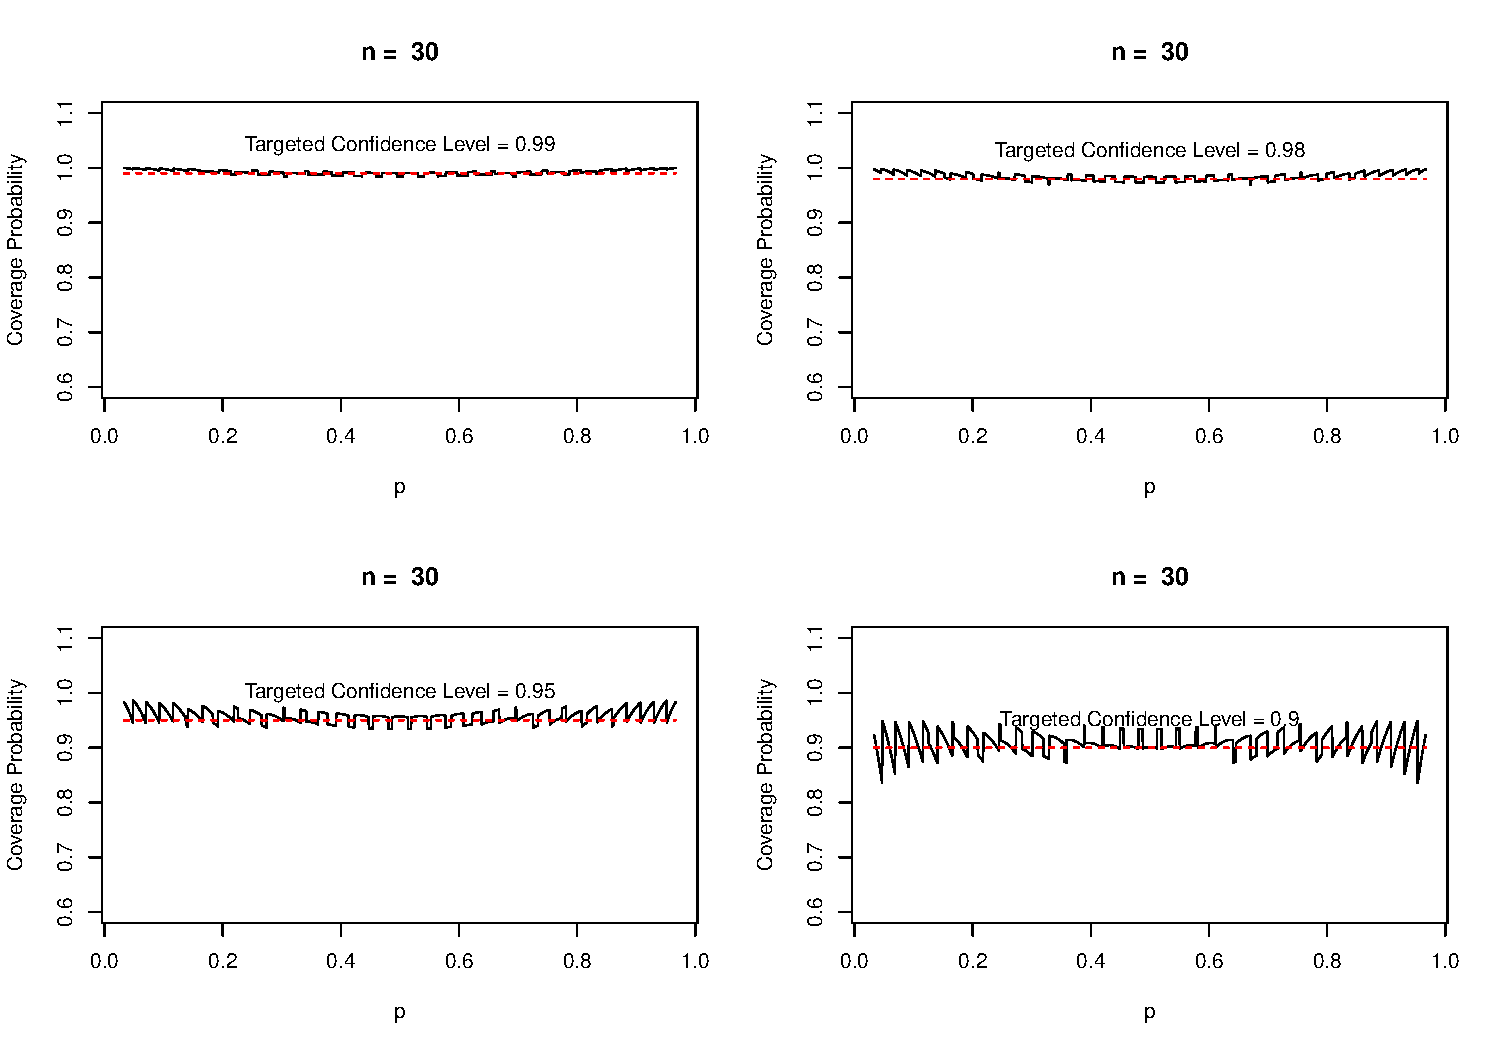
\includegraphics[width=0.9\linewidth,height=0.8\textheight]{Week11_12_13_files/figure-beamer/unnamed-chunk-19-1} \end{center}
\normalsize
\end{frame}

\begin{frame}[fragile]{Coverage Probabilities of Binomial Confidence
Intervals - Wilson}
\protect\hypertarget{coverage-probabilities-of-binomial-confidence-intervals---wilson}{}
Next we use Wilson score intervals to do the same thing.

\tiny

\begin{Shaded}
\begin{Highlighting}[]
\FunctionTok{par}\NormalTok{(}\AttributeTok{mfrow=}\FunctionTok{c}\NormalTok{(}\DecValTok{2}\NormalTok{, }\DecValTok{2}\NormalTok{))}
\ControlFlowTok{for}\NormalTok{(alpha }\ControlFlowTok{in} \FunctionTok{c}\NormalTok{(}\FloatTok{0.01}\NormalTok{, }\FloatTok{0.02}\NormalTok{, }\FloatTok{0.05}\NormalTok{, }\FloatTok{0.10}\NormalTok{))\{}
\NormalTok{n }\OtherTok{\textless{}{-}} \DecValTok{30}     \CommentTok{\# number of trials}
\NormalTok{CL }\OtherTok{\textless{}{-}} \DecValTok{1} \SpecialCharTok{{-}}\NormalTok{ alpha}
\NormalTok{x }\OtherTok{\textless{}{-}} \DecValTok{0}\SpecialCharTok{:}\NormalTok{n }
\NormalTok{z }\OtherTok{\textless{}{-}} \FunctionTok{qnorm}\NormalTok{(}\DecValTok{1} \SpecialCharTok{{-}}\NormalTok{ alpha}\SpecialCharTok{/}\DecValTok{2}\NormalTok{)}
\NormalTok{sp }\OtherTok{\textless{}{-}}\NormalTok{ x}\SpecialCharTok{/}\NormalTok{n}
\NormalTok{sptilda }\OtherTok{\textless{}{-}}\NormalTok{ (x }\SpecialCharTok{+}\NormalTok{ z}\SpecialCharTok{\^{}}\DecValTok{2}\SpecialCharTok{/}\DecValTok{2}\NormalTok{)}\SpecialCharTok{/}\NormalTok{(n }\SpecialCharTok{+}\NormalTok{ z}\SpecialCharTok{\^{}}\DecValTok{2}\NormalTok{)}
\NormalTok{m.err }\OtherTok{\textless{}{-}}\NormalTok{ (z}\SpecialCharTok{/}\NormalTok{(n }\SpecialCharTok{+}\NormalTok{ z}\SpecialCharTok{\^{}}\DecValTok{2}\NormalTok{))}\SpecialCharTok{*}\FunctionTok{sqrt}\NormalTok{(n}\SpecialCharTok{*}\NormalTok{sp}\SpecialCharTok{*}\NormalTok{(}\DecValTok{1} \SpecialCharTok{{-}}\NormalTok{ sp) }\SpecialCharTok{+}\NormalTok{ z}\SpecialCharTok{\^{}}\DecValTok{2}\SpecialCharTok{/}\DecValTok{4}\NormalTok{)}
\NormalTok{lcl }\OtherTok{\textless{}{-}}\NormalTok{ sptilda }\SpecialCharTok{{-}}\NormalTok{ m.err}
\NormalTok{ucl }\OtherTok{\textless{}{-}}\NormalTok{ sptilda }\SpecialCharTok{+}\NormalTok{ m.err}
\NormalTok{m }\OtherTok{\textless{}{-}} \DecValTok{2000} \CommentTok{\# number of values of pp}
\NormalTok{pp }\OtherTok{\textless{}{-}} \FunctionTok{seq}\NormalTok{(}\DecValTok{1}\SpecialCharTok{/}\NormalTok{n, }\DecValTok{1} \SpecialCharTok{{-}} \DecValTok{1}\SpecialCharTok{/}\NormalTok{n, }\AttributeTok{length =}\NormalTok{ m)}
\NormalTok{p.cov }\OtherTok{\textless{}{-}} \FunctionTok{numeric}\NormalTok{(m)}
\ControlFlowTok{for}\NormalTok{(i }\ControlFlowTok{in} \DecValTok{1}\SpecialCharTok{:}\NormalTok{m)\{}
\NormalTok{  cover }\OtherTok{\textless{}{-}}\NormalTok{ (pp[i] }\SpecialCharTok{\textgreater{}=}\NormalTok{ lcl) }\SpecialCharTok{\&}\NormalTok{ (pp[i] }\SpecialCharTok{\textless{}=}\NormalTok{ ucl)  }\CommentTok{\# vector of 0s and 1s}
\NormalTok{  p.rel }\OtherTok{\textless{}{-}} \FunctionTok{dbinom}\NormalTok{(x[cover], n, pp[i])}
\NormalTok{  p.cov[i] }\OtherTok{\textless{}{-}} \FunctionTok{sum}\NormalTok{(p.rel)}
\NormalTok{\}}
\FunctionTok{plot}\NormalTok{(pp, p.cov, }\AttributeTok{type =} \StringTok{"l"}\NormalTok{, }\AttributeTok{ylim =}\FunctionTok{c}\NormalTok{(}\FloatTok{0.60}\NormalTok{, }\FloatTok{1.1}\NormalTok{), }\AttributeTok{main =} \FunctionTok{paste}\NormalTok{(}\StringTok{"n = "}\NormalTok{, n), }
     \AttributeTok{xlab =} \StringTok{"p"}\NormalTok{, }\AttributeTok{ylab =} \StringTok{"Coverage Probability"}\NormalTok{)}
\FunctionTok{lines}\NormalTok{(}\FunctionTok{c}\NormalTok{(}\DecValTok{1}\SpecialCharTok{/}\NormalTok{n, }\DecValTok{1}\SpecialCharTok{{-}} \DecValTok{1}\SpecialCharTok{/}\NormalTok{n), }\FunctionTok{c}\NormalTok{(}\DecValTok{1} \SpecialCharTok{{-}}\NormalTok{ alpha, }\DecValTok{1}\SpecialCharTok{{-}}\NormalTok{ alpha), }\AttributeTok{col =} \StringTok{"red"}\NormalTok{, }\AttributeTok{lty =} \StringTok{"dashed"}\NormalTok{)}
      \FunctionTok{text}\NormalTok{(}\FloatTok{0.5}\NormalTok{, CL }\SpecialCharTok{+} \FloatTok{0.05}\NormalTok{, }\FunctionTok{paste}\NormalTok{(}\StringTok{"Targeted Confidence Level ="}\NormalTok{, CL))}
\NormalTok{\}}
\end{Highlighting}
\end{Shaded}

\normalsize
\end{frame}

\begin{frame}{Coverage Probabilities of Binomial Confidence Intervals -
Wilson}
\protect\hypertarget{coverage-probabilities-of-binomial-confidence-intervals---wilson-1}{}
\tiny

\begin{center}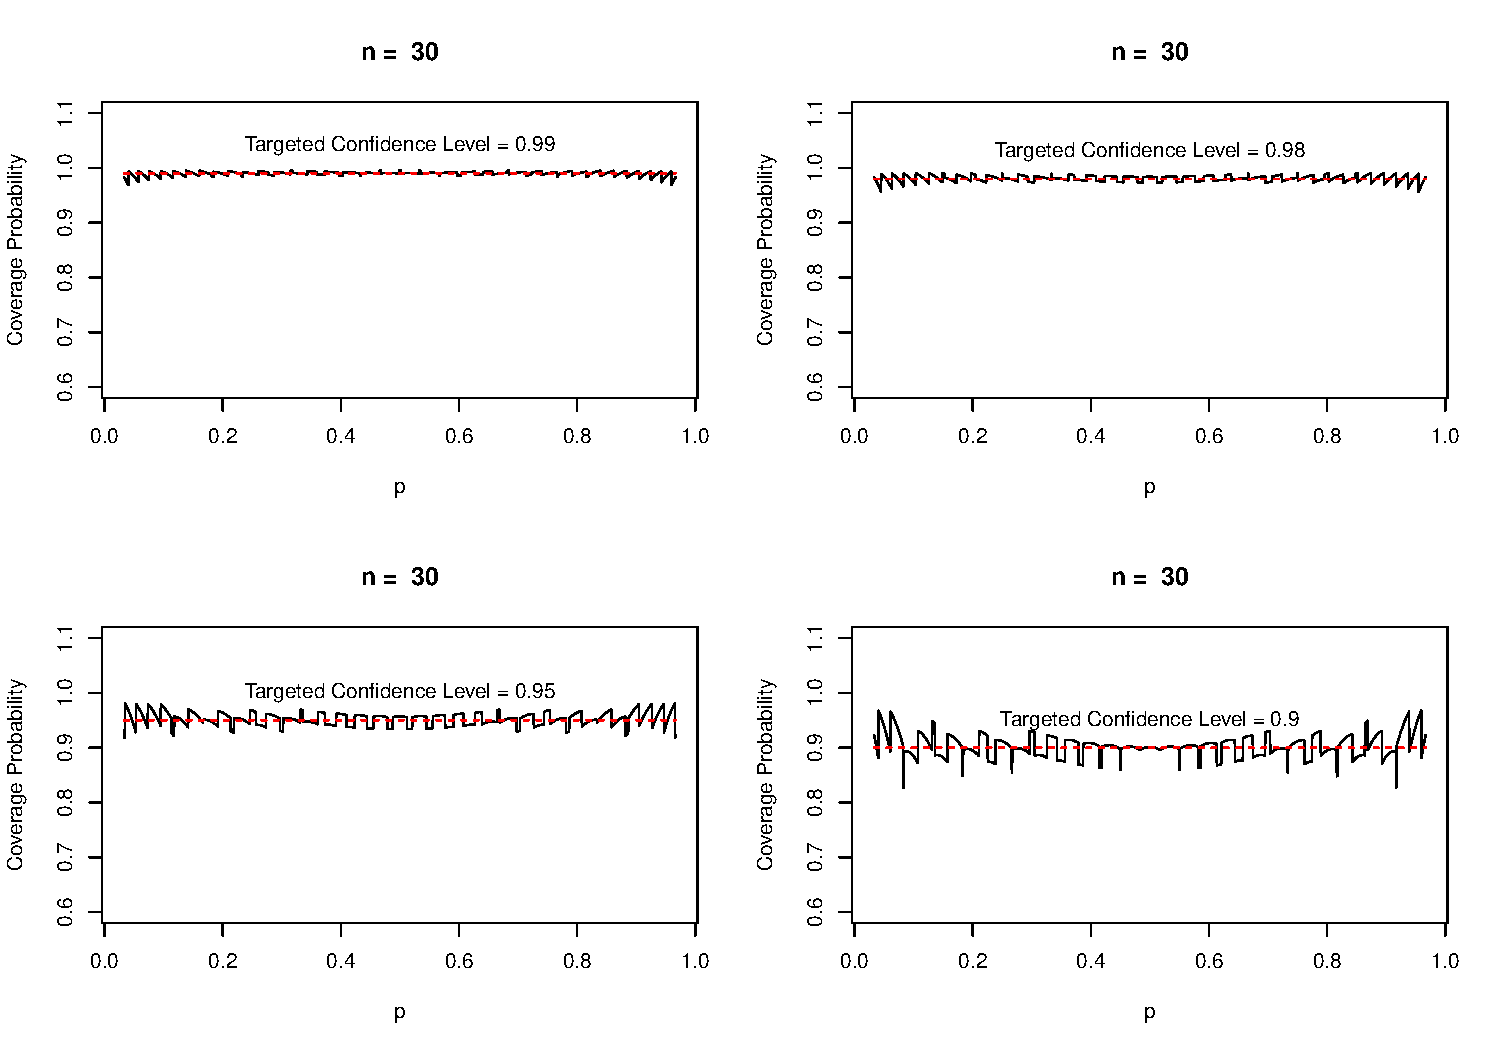
\includegraphics[width=0.9\linewidth,height=0.8\textheight]{Week11_12_13_files/figure-beamer/unnamed-chunk-21-1} \end{center}
\normalsize
\end{frame}

\hypertarget{bootstrap-t-confidence-interval}{%
\section{\texorpdfstring{Bootstrap \(t\) Confidence
Interval}{Bootstrap t Confidence Interval}}\label{bootstrap-t-confidence-interval}}

\begin{frame}[fragile]{Bootstrap \(t\) Confidence Interval}
\protect\hypertarget{bootstrap-t-confidence-interval-1}{}
\begin{itemize}
\item
  The bootstrap percentile confidence interval for giving a range of
  plausible values for a parameter was introduced earlier.
\item
  Another confidence interval is the bootstrap \(t\) interval that is
  based on estimating the actual distribution of the \(t\) statistic
  from the data, rather than just assuming that the \(t\) statistic has
  a Student's \(t\) distribution.
\end{itemize}

Recall the \texttt{Bangladesh} arsenic levels data. The distribution of
arsenic levels was skewed right.

\tiny

\begin{Shaded}
\begin{Highlighting}[]
\FunctionTok{library}\NormalTok{(resampledata)}
\FunctionTok{head}\NormalTok{(Bangladesh)}
\end{Highlighting}
\end{Shaded}

\begin{verbatim}
  Arsenic Chlorine Cobalt
1    2400      6.2   0.42
2       6    116.0   0.45
3     904     14.8   0.63
4     321     35.9   0.68
5    1280     18.9   0.58
6     151      7.8   0.35
\end{verbatim}

\normalsize
\end{frame}

\begin{frame}[fragile]{Bootstrap \(t\) Confidence Interval}
\protect\hypertarget{bootstrap-t-confidence-interval-2}{}
\tiny

\begin{Shaded}
\begin{Highlighting}[]
\FunctionTok{ggplot}\NormalTok{(}\AttributeTok{data =}\NormalTok{ Bangladesh, }\FunctionTok{aes}\NormalTok{(}\AttributeTok{x =}\NormalTok{ Arsenic)) }\SpecialCharTok{+} 
  \FunctionTok{geom\_histogram}\NormalTok{(}\AttributeTok{fill =} \StringTok{"blue"}\NormalTok{, }\AttributeTok{color =} \StringTok{"black"}\NormalTok{,}
                 \AttributeTok{binwidth =} \DecValTok{100}\NormalTok{) }\SpecialCharTok{+} 
  \FunctionTok{theme\_bw}\NormalTok{()}
\end{Highlighting}
\end{Shaded}

\begin{center}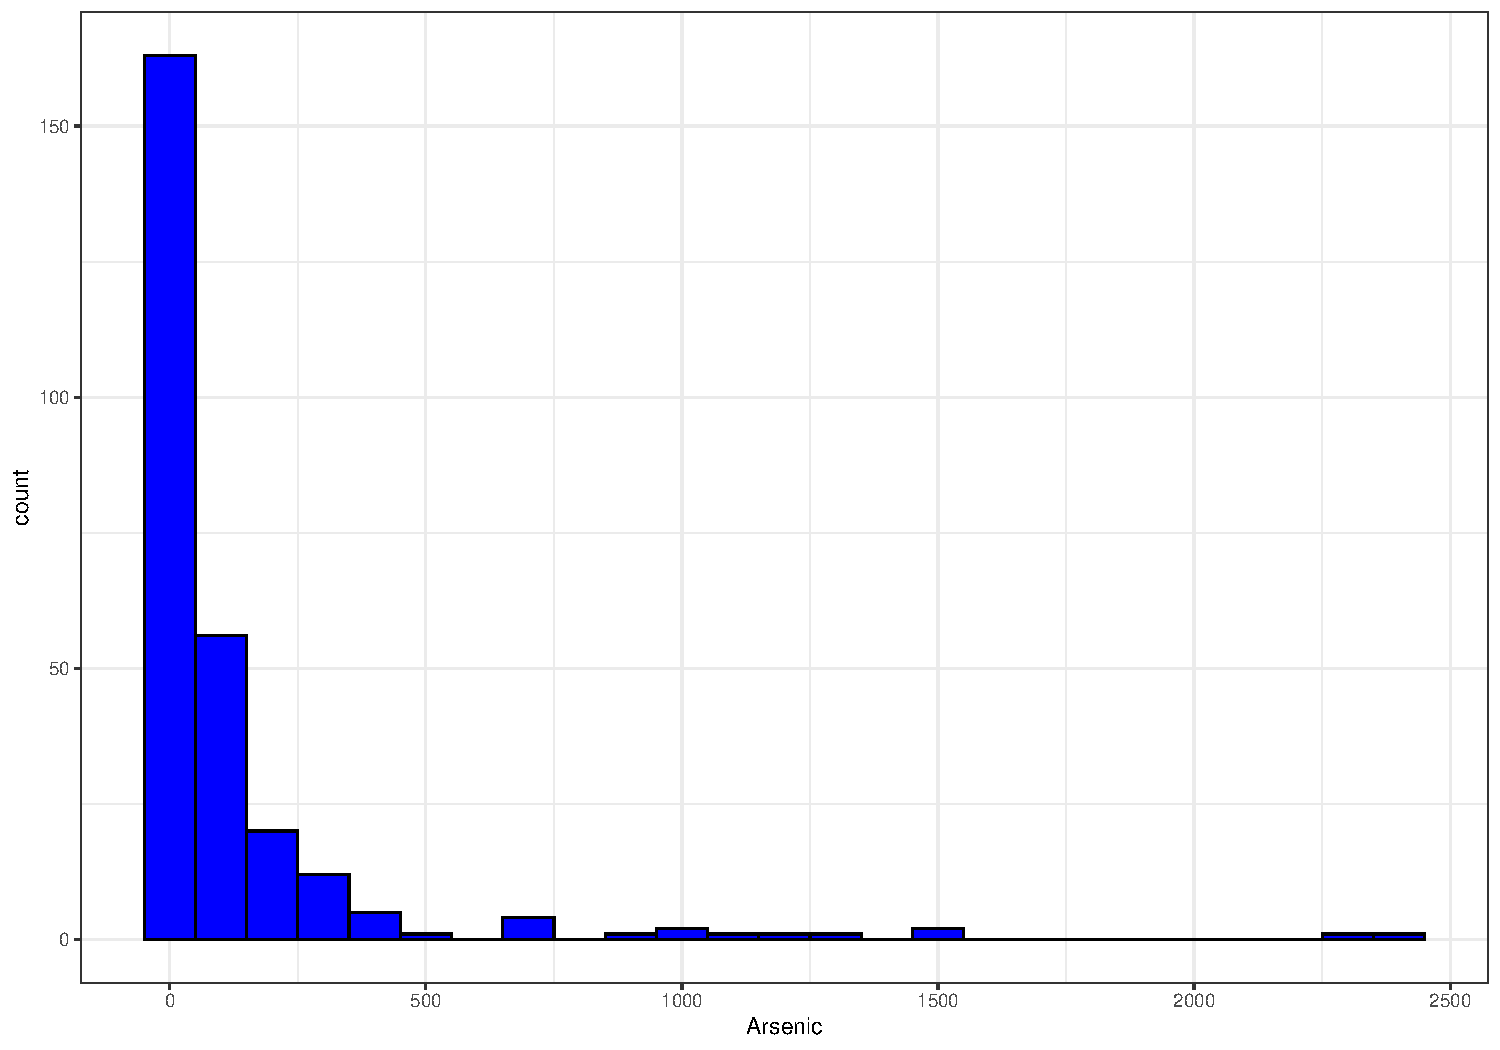
\includegraphics[width=0.6\linewidth,height=0.4\textheight]{Week11_12_13_files/figure-beamer/unnamed-chunk-23-1} \end{center}
\normalsize

To use the \(t\) interval formula for the mean \(\mu\) requires that the
statistic \[T=\frac{\bar{x}-\mu}{S/\sqrt{n}}\] to follow a \(t_{\nu}\).
That seems unlikely for data this skewed.
\end{frame}

\begin{frame}{Bootstrap \(t\) Confidence Interval}
\protect\hypertarget{bootstrap-t-confidence-interval-3}{}
Instead

\begin{itemize}
\item
  we bootstrap the \(t\) statistic: for each of the \(10^5\) resamples,
\item
  we compute

  \begin{itemize}
  \tightlist
  \item
    the resample mean \(\bar{X}^*\)
  \item
    resample standard deviation \(S^*\)
  \end{itemize}
\item
  and then compute the resample \(T\) statistic
  \[T^*=\frac{\bar{X}^*-\bar{x}}{S^*/\sqrt{n}}\]
\end{itemize}
\end{frame}

\begin{frame}[fragile]{Bootstrap \(t\) Confidence Interval}
\protect\hypertarget{bootstrap-t-confidence-interval-4}{}
\tiny

\begin{Shaded}
\begin{Highlighting}[]
\NormalTok{Arsenic }\OtherTok{\textless{}{-}} \FunctionTok{subset}\NormalTok{(Bangladesh, }\AttributeTok{select =}\NormalTok{ Arsenic, }\AttributeTok{drop =}\NormalTok{ T)}
\NormalTok{xbar }\OtherTok{\textless{}{-}} \FunctionTok{mean}\NormalTok{(Arsenic)}
\NormalTok{S }\OtherTok{\textless{}{-}} \FunctionTok{sd}\NormalTok{(Arsenic)}
\NormalTok{N }\OtherTok{\textless{}{-}} \DecValTok{10}\SpecialCharTok{\^{}}\DecValTok{5}
\NormalTok{n }\OtherTok{\textless{}{-}} \FunctionTok{length}\NormalTok{(Arsenic)}
\NormalTok{Tstar }\OtherTok{\textless{}{-}} \FunctionTok{numeric}\NormalTok{(N)}
\NormalTok{Sstar }\OtherTok{\textless{}{-}} \FunctionTok{numeric}\NormalTok{(N)}
\NormalTok{Xbarstar }\OtherTok{\textless{}{-}} \FunctionTok{numeric}\NormalTok{(N)}
\FunctionTok{set.seed}\NormalTok{(}\DecValTok{13}\NormalTok{)}
\ControlFlowTok{for}\NormalTok{ (i }\ControlFlowTok{in} \DecValTok{1}\SpecialCharTok{:}\NormalTok{N)}
\NormalTok{\{}
\NormalTok{  x }\OtherTok{\textless{}{-}}\FunctionTok{sample}\NormalTok{(Arsenic, }\AttributeTok{size =}\NormalTok{ n, }\AttributeTok{replace =}\NormalTok{ T)}
\NormalTok{  Xbarstar[i] }\OtherTok{\textless{}{-}} \FunctionTok{mean}\NormalTok{(x)}
\NormalTok{  Sstar[i] }\OtherTok{\textless{}{-}} \FunctionTok{sd}\NormalTok{(x)}
\NormalTok{\}}
\NormalTok{Tstar }\OtherTok{\textless{}{-}}\NormalTok{ (Xbarstar }\SpecialCharTok{{-}}\NormalTok{ xbar)}\SpecialCharTok{/}\NormalTok{(Sstar }\SpecialCharTok{/} \FunctionTok{sqrt}\NormalTok{(n))}
\NormalTok{CIt }\OtherTok{\textless{}{-}} \FunctionTok{quantile}\NormalTok{(Tstar, }\FunctionTok{c}\NormalTok{(}\FloatTok{0.025}\NormalTok{, }\FloatTok{0.975}\NormalTok{))}
\FunctionTok{names}\NormalTok{(CIt) }\OtherTok{\textless{}{-}} \ConstantTok{NULL}
\NormalTok{CIt}
\end{Highlighting}
\end{Shaded}

\begin{verbatim}
[1] -2.654657  1.655932
\end{verbatim}

\begin{Shaded}
\begin{Highlighting}[]
\NormalTok{(BPCI }\OtherTok{\textless{}{-}} \FunctionTok{quantile}\NormalTok{(Xbarstar, }\AttributeTok{probs =} \FunctionTok{c}\NormalTok{(}\FloatTok{0.025}\NormalTok{, }\FloatTok{0.975}\NormalTok{)))}
\end{Highlighting}
\end{Shaded}

\begin{verbatim}
    2.5%    97.5% 
 92.3708 163.1075 
\end{verbatim}

\normalsize
\end{frame}

\begin{frame}[fragile]{Bootstrap \(t\) Confidence Interval}
\protect\hypertarget{bootstrap-t-confidence-interval-5}{}
\tiny

\begin{Shaded}
\begin{Highlighting}[]
\FunctionTok{par}\NormalTok{(}\AttributeTok{mfrow=} \FunctionTok{c}\NormalTok{(}\DecValTok{2}\NormalTok{, }\DecValTok{2}\NormalTok{))}
\FunctionTok{plot}\NormalTok{(Xbarstar, Sstar, }\AttributeTok{ylab =} \StringTok{"S*"}\NormalTok{, }\AttributeTok{xlab =} \FunctionTok{substitute}\NormalTok{(}\FunctionTok{paste}\NormalTok{(}\FunctionTok{bar}\NormalTok{(X),}\StringTok{"*"}\NormalTok{)), }\AttributeTok{col =} \FunctionTok{rgb}\NormalTok{(}\DecValTok{1}\NormalTok{,}\DecValTok{0}\NormalTok{,}\DecValTok{0}\NormalTok{,}\FloatTok{0.01}\NormalTok{))}
\FunctionTok{qqnorm}\NormalTok{(Tstar, }\AttributeTok{col =} \FunctionTok{rgb}\NormalTok{(}\DecValTok{1}\NormalTok{,}\DecValTok{0}\NormalTok{,}\DecValTok{0}\NormalTok{,}\FloatTok{0.01}\NormalTok{))}
\FunctionTok{qqline}\NormalTok{(Tstar)}
\FunctionTok{hist}\NormalTok{(Tstar, }\AttributeTok{xlab =} \StringTok{"T*"}\NormalTok{, }\AttributeTok{main =} \StringTok{"Bootstrap distribution of T*"}\NormalTok{, }\AttributeTok{col =} \StringTok{"red"}\NormalTok{, }\AttributeTok{breaks =} \StringTok{"Scott"}\NormalTok{)}
\FunctionTok{hist}\NormalTok{(Xbarstar, }\AttributeTok{xlab =} \FunctionTok{substitute}\NormalTok{(}\FunctionTok{paste}\NormalTok{(}\FunctionTok{bar}\NormalTok{(X),}\StringTok{"*"}\NormalTok{)), }
     \AttributeTok{main =} \FunctionTok{substitute}\NormalTok{(}\FunctionTok{paste}\NormalTok{(}\StringTok{"Bootstrap Distribution of "}\NormalTok{, }\FunctionTok{bar}\NormalTok{(X),}\StringTok{"*"}\NormalTok{)), }\AttributeTok{col =} \StringTok{"red"}\NormalTok{, }\AttributeTok{breaks =} \StringTok{"Scott"}\NormalTok{)}
\end{Highlighting}
\end{Shaded}

\normalsize
\end{frame}

\begin{frame}{Bootstrap \(t\) Confidence Interval}
\protect\hypertarget{bootstrap-t-confidence-interval-6}{}
\tiny

\begin{center}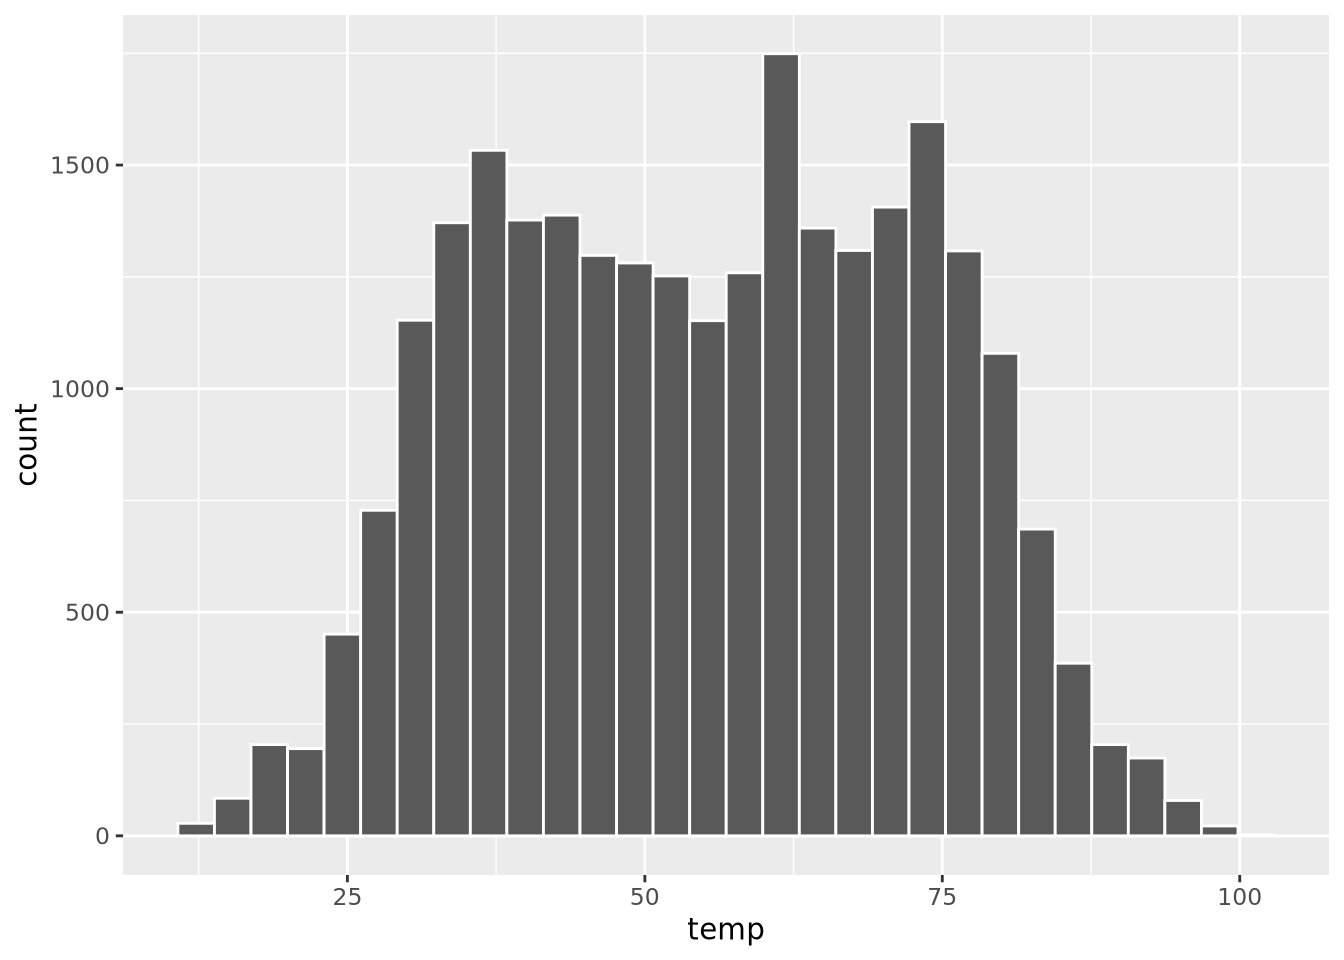
\includegraphics[width=0.9\linewidth,height=0.8\textheight]{Week11_12_13_files/figure-beamer/unnamed-chunk-26-1} \end{center}
\normalsize
\end{frame}

\begin{frame}{Bootstrap \(t\) Confidence Interval}
\protect\hypertarget{bootstrap-t-confidence-interval-7}{}
\begin{itemize}
\item
  Note that the bootstrap distribution for the \(t\) statistic is left
  skewed;

  \begin{itemize}
  \tightlist
  \item
    in fact, it is more left skewed than the the bootstrap distribution
    of the mean which is right skewed!
  \end{itemize}
\item
  The reason for this is the strong positive relationship between
  \(\bar{X}^*\) and \(S^*\).

  \begin{itemize}
  \tightlist
  \item
    If a bootstrap resample contains a large number of the big values
    from the right tail of the original data, then \(\bar{X}^*\) is
    large and hence \(S^*\) is especially large (standard deviations are
    computed by squaring distances from the mean, so they are affected
    even more by large observations than a mean is).
  \item
    The large denominator thus keeps \(T^*\) from being particularly
    large.
  \item
    Conversely, when there are relatively few of the big observations in
    the resample, then \(\bar{X}^*-\bar{x}\) is negative and the
    denominator can be especially small, thus resulting in a \(T\) ratio
    that is large negative.
  \end{itemize}
\end{itemize}
\end{frame}

\begin{frame}{Bootstrap \(t\) Confidence Interval}
\protect\hypertarget{bootstrap-t-confidence-interval-8}{}
\begin{itemize}
\item
  The \(2.5\%\) and \(97.5\%\) percentiles of the bootstrap \(t\)
  distribution are -2.6546571 and 1.6559318, compared to \(\pm1.968789\)
  for the Student's \(t\) distribution.

  \begin{itemize}
  \tightlist
  \item
    This is a reflection of the skewed nature of the bootstrap \(t\)
    distribution compared to the symmetric Student's \(t\) distribution.
  \end{itemize}
\item
  What skewness implies for the accuracy of the formula-based \(t\)
  confidence intervals
  \((\bar{X}\pm t_{1-\alpha/2, \nu}\times S/\sqrt{n})\)?

  \begin{itemize}
  \tightlist
  \item
    For right-skewed data, when \(\bar{X}<\mu\), typically \(S< \sigma\)
    so the confidence interval tends to be narrow, and the interval
    falls below \(\mu\) more often than \(\alpha/2\times 100\%\) of the
    time. This is bad.
  \item
    Conversely, when \(\bar{X}>\mu\), typically \(S>\sigma\) so the
    intervals tend to be to wide and do not miss \(\mu\) often enough;
    this is also bad.
  \item
    Overall, the intervals tend to be to the left of where they should
    be and give a biased picture of where the mean is likely to be.
  \end{itemize}
\end{itemize}
\end{frame}

\begin{frame}{Bootstrap \(t\) Confidence Interval}
\protect\hypertarget{bootstrap-t-confidence-interval-9}{}
\begin{itemize}
\item
  Let

  \begin{itemize}
  \tightlist
  \item
    \(T=\frac{\bar{X}-\mu}{S/\sqrt{n}}\) and
  \item
    \(F\) be the cdf for the \(T\) statistic (the cdf of the sampling
    distribution)
  \item
    \(Q_1\) and \(Q_2\) denote the \(\alpha/2\) and \((1-\alpha/2)\)
    quantiles of this distribution; that is, \(Q_1=F^{-1}(\alpha/2)\)
    and \(Q_2=F^{-1}(1-\alpha/2)\).
  \end{itemize}
\item
  Then:
  \[1-\alpha=P(Q_1<T<Q_2)=P\left(Q_1<\frac{\bar{X}-\mu}{S/\sqrt{n}}<Q_2\right)\]
\item
  This suggest the confidence interval:
  \[CI_{1-\alpha}(\mu)=\left(\bar{X}-Q_2\frac{S}{\sqrt{n}},\bar{X}-Q_1\frac{S}{\sqrt{n}}\right)\]
  \tiny The quantiles \(Q_1\) and \(Q_2\) are unknown, but they can be
  estimated using quantiles of the bootstrap distribution of the \(t\)
  statistic: \(T^*=(\bar{X}^*-\bar{x})/(S^*/\sqrt{n})\) where
  \(\bar{X}^*\) and \(S^*\) are the mean and standard deviation of a
  bootstrap resample. \normalsize
\end{itemize}
\end{frame}

\begin{frame}[fragile]{Bootstrap \(t\) Confidence Interval}
\protect\hypertarget{bootstrap-t-confidence-interval-10}{}
\begin{itemize}
\item
  We use the standard error formula for every bootstrap sample because
  the bootstrap statistic should mimic
  \(T=\frac{\bar{X}-\mu}{S/\sqrt{n}}\).
\item
  Thus: \(Q_1=-2.6546571\) and \(Q_2=1.6559318\), so we compute
\end{itemize}

\small

\begin{Shaded}
\begin{Highlighting}[]
\NormalTok{LL }\OtherTok{\textless{}{-}}\NormalTok{ xbar }\SpecialCharTok{{-}}\NormalTok{ CIt[}\DecValTok{2}\NormalTok{]}\SpecialCharTok{*}\NormalTok{S}\SpecialCharTok{/}\FunctionTok{sqrt}\NormalTok{(n)}
\NormalTok{UL }\OtherTok{\textless{}{-}}\NormalTok{ xbar }\SpecialCharTok{{-}}\NormalTok{ CIt[}\DecValTok{1}\NormalTok{]}\SpecialCharTok{*}\NormalTok{S}\SpecialCharTok{/}\FunctionTok{sqrt}\NormalTok{(n)}
\NormalTok{(}\FunctionTok{c}\NormalTok{(LL, UL))}
\end{Highlighting}
\end{Shaded}

\begin{verbatim}
[1]  95.34636 173.37114
\end{verbatim}

\normalsize

\begin{itemize}
\item
  The \(95\%\) bootstrap percentile interval is
  \((92.3708026, 163.1074815)\) while the formula \(t\) confidence
  interval is \((89.6834234, 160.956429)\)
\item
  The bootstrap \(t\) interval is stretched further to the right,
  reflecting the right-skewed distribution of the data.
\item
  Because of the large sample size, we report the \(95\%\) bootstrap
  \(t\) confidence interval \((95.346365, 173.371137)\mu\) \(g/dL\).
\end{itemize}
\end{frame}

\begin{frame}[fragile]{Using the package \texttt{boot}}
\protect\hypertarget{using-the-package-boot}{}
Next we consider computing the bootstrap percentile and \(t\) confidence
intervals using the functions \texttt{boot()} and \texttt{boot.ci()}
functions from the package \texttt{boot}.

\begin{itemize}
\item
  We write the function \texttt{mean.boot()} and use
  \texttt{mean.boot()} inside the \texttt{boot()} function storing the
  results in the object \texttt{boot.out}.
\item
  Finally, the function \texttt{boot.ci()} is applied to
  \texttt{boot.out} which results in the creation of the percentile and
  confidence intervals.
\end{itemize}
\end{frame}

\begin{frame}[fragile]{Using the package \texttt{boot}}
\protect\hypertarget{using-the-package-boot-1}{}
\tiny

\begin{Shaded}
\begin{Highlighting}[]
\FunctionTok{require}\NormalTok{(boot)}
\NormalTok{mean.boot }\OtherTok{\textless{}{-}} \ControlFlowTok{function}\NormalTok{(data, i)\{}
\NormalTok{  d }\OtherTok{\textless{}{-}}\NormalTok{ data[i]}
\NormalTok{  M }\OtherTok{\textless{}{-}} \FunctionTok{mean}\NormalTok{(d)}
\NormalTok{  V }\OtherTok{\textless{}{-}} \FunctionTok{var}\NormalTok{(d)}\SpecialCharTok{/}\FunctionTok{length}\NormalTok{(i)}
  \FunctionTok{return}\NormalTok{(}\FunctionTok{c}\NormalTok{(M, V))}
\NormalTok{\}}
\NormalTok{boot.out }\OtherTok{\textless{}{-}} \FunctionTok{boot}\NormalTok{(Arsenic, mean.boot, }\AttributeTok{R=}\DecValTok{10}\SpecialCharTok{\^{}}\DecValTok{5}\NormalTok{)}
\FunctionTok{boot.ci}\NormalTok{(boot.out, }\AttributeTok{conf =} \FloatTok{0.95}\NormalTok{, }\AttributeTok{type =} \FunctionTok{c}\NormalTok{(}\StringTok{"perc"}\NormalTok{, }\StringTok{"stud"}\NormalTok{))}
\end{Highlighting}
\end{Shaded}

\begin{verbatim}
BOOTSTRAP CONFIDENCE INTERVAL CALCULATIONS
Based on 100000 bootstrap replicates

CALL : 
boot.ci(boot.out = boot.out, conf = 0.95, type = c("perc", "stud"))

Intervals : 
Level    Studentized          Percentile     
95%   ( 95.3, 173.1 )   ( 92.5, 163.2 )  
Calculations and Intervals on Original Scale
\end{verbatim}

\normalsize
\end{frame}

\begin{frame}[fragile]{Using the package \texttt{boot}}
\protect\hypertarget{using-the-package-boot-2}{}
\tiny

\begin{Shaded}
\begin{Highlighting}[]
\FunctionTok{plot}\NormalTok{(boot.out)}
\end{Highlighting}
\end{Shaded}

\begin{center}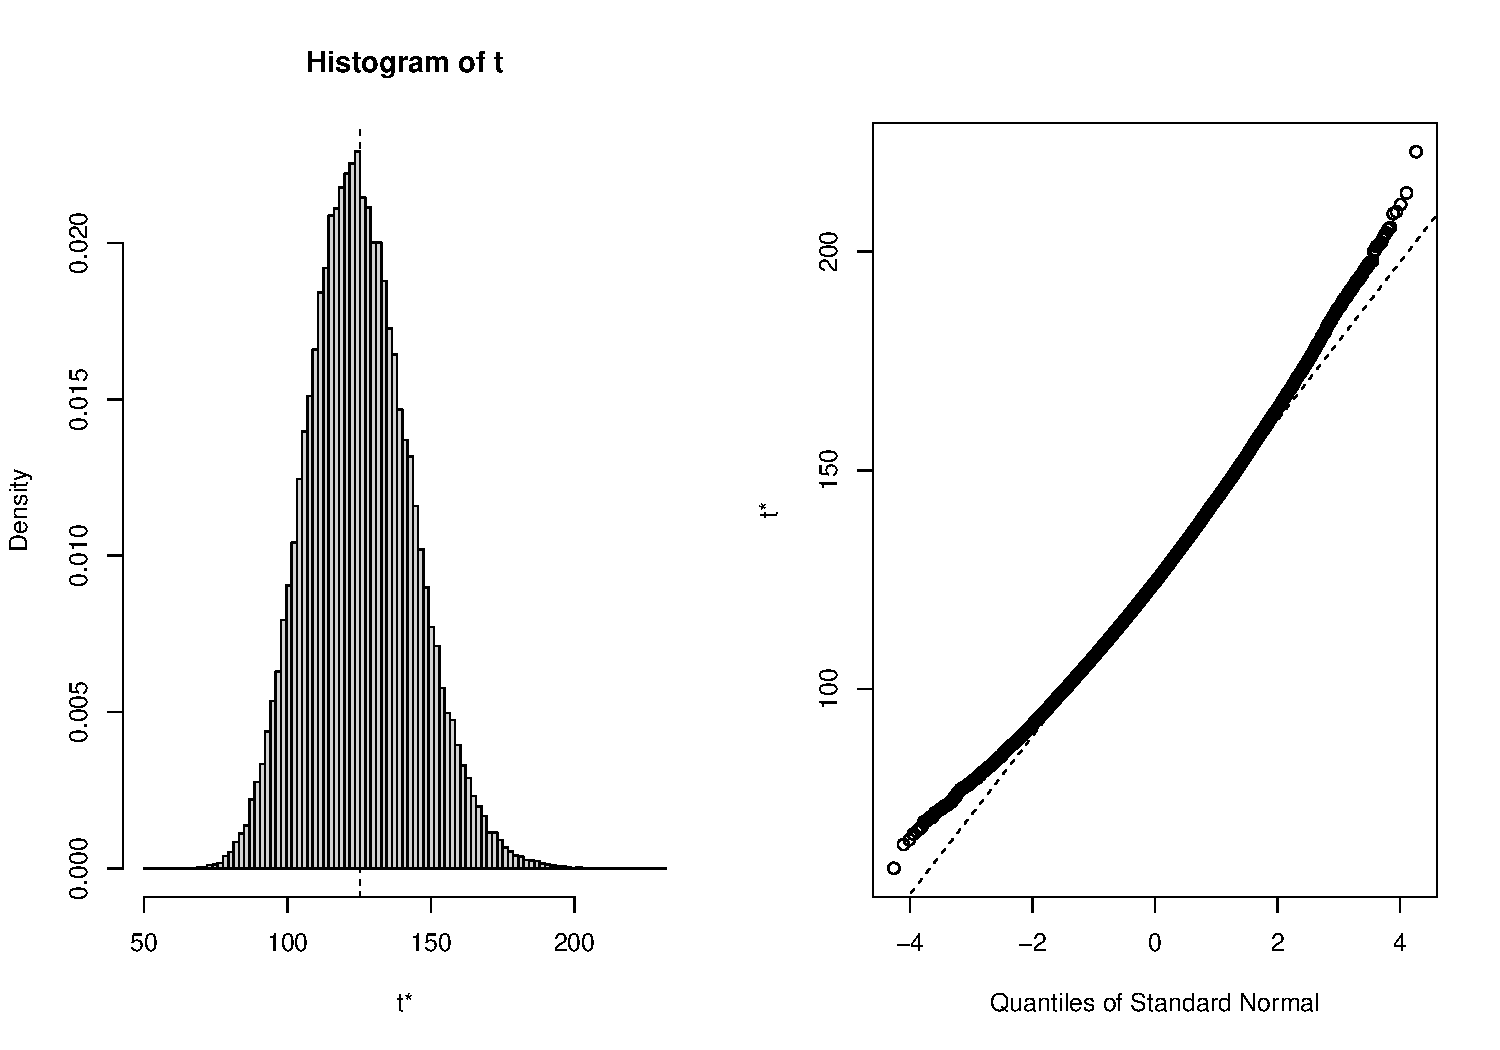
\includegraphics[width=0.8\linewidth,height=0.45\textheight]{Week11_12_13_files/figure-beamer/unnamed-chunk-29-1} \end{center}
\normalsize
\end{frame}

\begin{frame}[fragile]{Using the package \texttt{boot}}
\protect\hypertarget{using-the-package-boot-3}{}
\tiny

\begin{Shaded}
\begin{Highlighting}[]
\FunctionTok{par}\NormalTok{(}\AttributeTok{mfrow =} \FunctionTok{c}\NormalTok{(}\DecValTok{1}\NormalTok{, }\DecValTok{2}\NormalTok{))}
\FunctionTok{hist}\NormalTok{(boot.out}\SpecialCharTok{$}\NormalTok{t[,}\DecValTok{1}\NormalTok{], }\AttributeTok{col =} \StringTok{"pink"}\NormalTok{, }\AttributeTok{breaks =} \StringTok{"Scott"}\NormalTok{, }\AttributeTok{main =} \StringTok{""}\NormalTok{, }
     \AttributeTok{xlab =} \FunctionTok{substitute}\NormalTok{(}\FunctionTok{paste}\NormalTok{(}\FunctionTok{bar}\NormalTok{(X),}\StringTok{"*"}\NormalTok{)), }\AttributeTok{freq=} \ConstantTok{FALSE}\NormalTok{)}
\FunctionTok{lines}\NormalTok{(}\FunctionTok{density}\NormalTok{(boot.out}\SpecialCharTok{$}\NormalTok{t[,}\DecValTok{1}\NormalTok{]), }\AttributeTok{lwd =} \DecValTok{2}\NormalTok{)}
\FunctionTok{hist}\NormalTok{((boot.out}\SpecialCharTok{$}\NormalTok{t[,}\DecValTok{1}\NormalTok{] }\SpecialCharTok{{-}}\NormalTok{ boot.out}\SpecialCharTok{$}\NormalTok{t0[}\DecValTok{1}\NormalTok{])}\SpecialCharTok{/}\NormalTok{(boot.out}\SpecialCharTok{$}\NormalTok{t[,}\DecValTok{2}\NormalTok{])}\SpecialCharTok{\^{}}\NormalTok{.}\DecValTok{5}\NormalTok{, }\AttributeTok{col =} \StringTok{"pink"}\NormalTok{, }\AttributeTok{breaks =} \StringTok{"Scott"}\NormalTok{, }\AttributeTok{main =} \StringTok{""}\NormalTok{, }
     \AttributeTok{xlab =}\StringTok{"T*"}\NormalTok{, }\AttributeTok{freq=} \ConstantTok{FALSE}\NormalTok{)}
\FunctionTok{lines}\NormalTok{(}\FunctionTok{density}\NormalTok{((boot.out}\SpecialCharTok{$}\NormalTok{t[,}\DecValTok{1}\NormalTok{] }\SpecialCharTok{{-}}\NormalTok{ boot.out}\SpecialCharTok{$}\NormalTok{t0[}\DecValTok{1}\NormalTok{])}\SpecialCharTok{/}\NormalTok{(boot.out}\SpecialCharTok{$}\NormalTok{t[,}\DecValTok{2}\NormalTok{])}\SpecialCharTok{\^{}}\NormalTok{.}\DecValTok{5}\NormalTok{), }\AttributeTok{lwd =} \DecValTok{2}\NormalTok{)}
\end{Highlighting}
\end{Shaded}

\begin{center}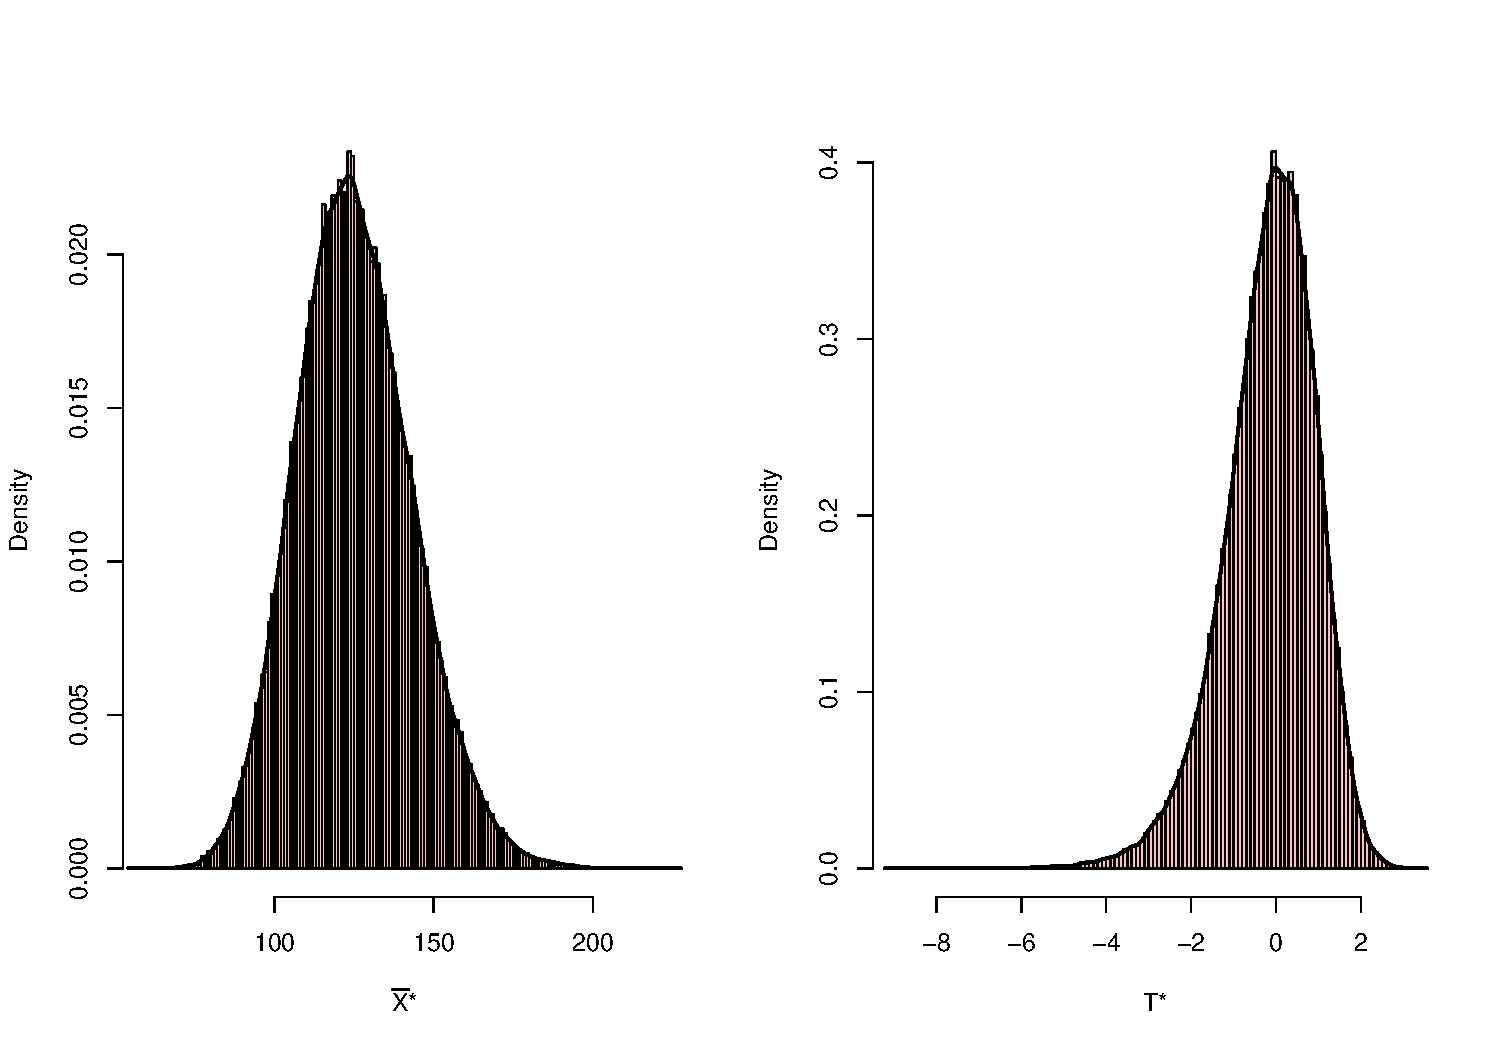
\includegraphics[width=0.8\linewidth,height=0.45\textheight]{Week11_12_13_files/figure-beamer/unnamed-chunk-30-1} \end{center}
\normalsize

The bootstrap intervals for a difference in means follows the same idea.
\end{frame}

\begin{frame}[fragile]{Bootstrap \(t\) confidence interval for
\(\mu_1-\mu_2\)}
\protect\hypertarget{bootstrap-t-confidence-interval-for-mu_1-mu_2}{}
For each of many resamples, calculate the bootstrap \(t\) statistic
\[T^*=\frac{\bar{X}^*_1-\bar{X}^*_2-(\bar{x}_1-\bar{x}_2)}{\sqrt{S^{2*}_1/n_1+S^{2*}_2/n_2}}\]

Let \(Q_1^*\) and \(Q_2^*\) be the empirical \(\alpha/2\) and
\((1-\alpha/2)\) quantiles of the bootstrap \(t\) distribution,
respectively. The bootstrap \(t\) confidence interval is

\[\scriptstyle CI_{1-\alpha}(\mu_1-\mu_2)=\left((\bar{x}_1-\bar{x}_2))-Q_2^*\times\sqrt{S^{2*}_1/n_1+S^{2*}_2/n_2},(\bar{x}_1-\bar{x}_2))-Q_1^*\times\sqrt{S^{2*}_1/n_1+S^{2*}_2/n_2}\right)\]

Recall the \texttt{Verizon} example, where we considered the difference
in means of two very skewed distributions of repair times for two very
unbalanced samples (\(n_1=23\) versus \(n_2=1664\)). Let us look at the
data again.
\end{frame}

\begin{frame}[fragile]{Verizon example}
\protect\hypertarget{verizon-example}{}
\tiny

\begin{Shaded}
\begin{Highlighting}[]
\NormalTok{Time.ILEC }\OtherTok{\textless{}{-}} \FunctionTok{subset}\NormalTok{(Verizon, }\AttributeTok{select=}\NormalTok{Time, Group }\SpecialCharTok{==} \StringTok{"ILEC"}\NormalTok{, }\AttributeTok{drop=}\ConstantTok{TRUE}\NormalTok{)}
\NormalTok{Time.CLEC }\OtherTok{\textless{}{-}} \FunctionTok{subset}\NormalTok{(Verizon, }\AttributeTok{select=}\NormalTok{Time, Group }\SpecialCharTok{==} \StringTok{"CLEC"}\NormalTok{, }\AttributeTok{drop=}\ConstantTok{TRUE}\NormalTok{)}
\NormalTok{thetahat }\OtherTok{\textless{}{-}} \FunctionTok{mean}\NormalTok{(Time.ILEC) }\SpecialCharTok{{-}} \FunctionTok{mean}\NormalTok{(Time.CLEC)}
\NormalTok{nx }\OtherTok{\textless{}{-}} \FunctionTok{length}\NormalTok{(Time.ILEC)  }\CommentTok{\#nx=1664}
\NormalTok{ny }\OtherTok{\textless{}{-}} \FunctionTok{length}\NormalTok{(Time.CLEC)  }\CommentTok{\#ny=23}
\NormalTok{SE }\OtherTok{\textless{}{-}} \FunctionTok{sqrt}\NormalTok{(}\FunctionTok{var}\NormalTok{(Time.ILEC)}\SpecialCharTok{/}\NormalTok{nx }\SpecialCharTok{+} \FunctionTok{var}\NormalTok{(Time.CLEC)}\SpecialCharTok{/}\NormalTok{ny)}
\NormalTok{N }\OtherTok{\textless{}{-}} \DecValTok{10}\SpecialCharTok{\^{}}\DecValTok{4}
\NormalTok{Tstar }\OtherTok{\textless{}{-}} \FunctionTok{numeric}\NormalTok{(N)}
\NormalTok{DM }\OtherTok{\textless{}{-}} \FunctionTok{numeric}\NormalTok{(N)}
\FunctionTok{set.seed}\NormalTok{(}\DecValTok{1}\NormalTok{)}
\ControlFlowTok{for}\NormalTok{(i }\ControlFlowTok{in} \DecValTok{1}\SpecialCharTok{:}\NormalTok{N)}
\NormalTok{\{}
\NormalTok{  bootx }\OtherTok{\textless{}{-}} \FunctionTok{sample}\NormalTok{(Time.ILEC, nx, }\AttributeTok{replace=}\ConstantTok{TRUE}\NormalTok{)}
\NormalTok{  booty }\OtherTok{\textless{}{-}} \FunctionTok{sample}\NormalTok{(Time.CLEC, ny, }\AttributeTok{replace=}\ConstantTok{TRUE}\NormalTok{)}
\NormalTok{  Tstar[i] }\OtherTok{\textless{}{-}}\NormalTok{ (}\FunctionTok{mean}\NormalTok{(bootx) }\SpecialCharTok{{-}} \FunctionTok{mean}\NormalTok{(booty) }\SpecialCharTok{{-}}\NormalTok{ thetahat) }\SpecialCharTok{/}
    \FunctionTok{sqrt}\NormalTok{(}\FunctionTok{var}\NormalTok{(bootx)}\SpecialCharTok{/}\NormalTok{nx }\SpecialCharTok{+} \FunctionTok{var}\NormalTok{(booty)}\SpecialCharTok{/}\NormalTok{ny)}
\NormalTok{  DM[i] }\OtherTok{\textless{}{-}} \FunctionTok{mean}\NormalTok{(bootx) }\SpecialCharTok{{-}} \FunctionTok{mean}\NormalTok{(booty)}
\NormalTok{\}}
\FunctionTok{quantile}\NormalTok{(Tstar, }\FunctionTok{c}\NormalTok{(.}\DecValTok{975}\NormalTok{, .}\DecValTok{025}\NormalTok{))}
\end{Highlighting}
\end{Shaded}

\begin{verbatim}
    97.5%      2.5% 
 3.514460 -1.479951 
\end{verbatim}

\normalsize
\end{frame}

\begin{frame}[fragile]{Verizon example}
\protect\hypertarget{verizon-example-1}{}
\tiny

\begin{Shaded}
\begin{Highlighting}[]
\NormalTok{CItboot }\OtherTok{\textless{}{-}}\NormalTok{ thetahat }\SpecialCharTok{{-}} \FunctionTok{quantile}\NormalTok{(Tstar, }\FunctionTok{c}\NormalTok{(.}\DecValTok{975}\NormalTok{, .}\DecValTok{025}\NormalTok{)) }\SpecialCharTok{*}\NormalTok{ SE}
\FunctionTok{names}\NormalTok{(CItboot) }\OtherTok{\textless{}{-}} \ConstantTok{NULL}
\NormalTok{CItboot}
\end{Highlighting}
\end{Shaded}

\begin{verbatim}
[1] -22.44597  -2.05534
\end{verbatim}

\begin{Shaded}
\begin{Highlighting}[]
\NormalTok{CIperct }\OtherTok{\textless{}{-}} \FunctionTok{quantile}\NormalTok{(DM, }\FunctionTok{c}\NormalTok{(}\FloatTok{0.025}\NormalTok{, }\FloatTok{0.975}\NormalTok{))}
\NormalTok{CIperct}
\end{Highlighting}
\end{Shaded}

\begin{verbatim}
      2.5%      97.5% 
-17.181759  -1.671277 
\end{verbatim}

\begin{Shaded}
\begin{Highlighting}[]
\FunctionTok{t.test}\NormalTok{(Time.ILEC, Time.CLEC)}\SpecialCharTok{$}\NormalTok{conf}
\end{Highlighting}
\end{Shaded}

\begin{verbatim}
[1] -16.5568985   0.3618588
attr(,"conf.level")
[1] 0.95
\end{verbatim}

\normalsize

The more accurate bootstrap \(t\) interval stretches farther in the
negative direction, even more than the bootstrap percentile interval.
\end{frame}

\begin{frame}[fragile]{Using the package boot for the difference in
means}
\protect\hypertarget{using-the-package-boot-for-the-difference-in-means}{}
Bootstrap percentile and \(t\) confidence intervals using the functions
\texttt{boot()} and \texttt{boot.ci()} functions from the package
\texttt{boot} are constructed using the user created
\texttt{mean2.boot()} function.

\tiny

\begin{Shaded}
\begin{Highlighting}[]
\FunctionTok{require}\NormalTok{(boot)}
\NormalTok{mean2.boot }\OtherTok{\textless{}{-}} \ControlFlowTok{function}\NormalTok{(data, i)\{}
\NormalTok{  d }\OtherTok{\textless{}{-}}\NormalTok{ data[i, ]}
\NormalTok{  M }\OtherTok{\textless{}{-}} \FunctionTok{tapply}\NormalTok{(d}\SpecialCharTok{$}\NormalTok{Time, d}\SpecialCharTok{$}\NormalTok{Group, mean)}
\NormalTok{  V }\OtherTok{\textless{}{-}} \FunctionTok{tapply}\NormalTok{(d}\SpecialCharTok{$}\NormalTok{Time, d}\SpecialCharTok{$}\NormalTok{Group, var)}\SpecialCharTok{/}\FunctionTok{tapply}\NormalTok{(d}\SpecialCharTok{$}\NormalTok{Time, d}\SpecialCharTok{$}\NormalTok{Group, length)}
  \FunctionTok{return}\NormalTok{(}\FunctionTok{c}\NormalTok{(M[}\DecValTok{2}\NormalTok{] }\SpecialCharTok{{-}}\NormalTok{ M[}\DecValTok{1}\NormalTok{], V[}\DecValTok{2}\NormalTok{] }\SpecialCharTok{+}\NormalTok{ V[}\DecValTok{1}\NormalTok{]))}
\NormalTok{\}}
\FunctionTok{set.seed}\NormalTok{(}\DecValTok{1}\NormalTok{)}
\NormalTok{boot.out }\OtherTok{\textless{}{-}} \FunctionTok{boot}\NormalTok{(Verizon, mean2.boot, }\AttributeTok{R=}\DecValTok{10}\SpecialCharTok{\^{}}\DecValTok{4}\NormalTok{, }\AttributeTok{strata =}\NormalTok{ Verizon[ ,}\DecValTok{2}\NormalTok{])}
\FunctionTok{boot.ci}\NormalTok{(boot.out, }\AttributeTok{conf =} \FloatTok{0.95}\NormalTok{, }\AttributeTok{type =} \FunctionTok{c}\NormalTok{(}\StringTok{"perc"}\NormalTok{, }\StringTok{"stud"}\NormalTok{))}
\end{Highlighting}
\end{Shaded}

\begin{verbatim}
BOOTSTRAP CONFIDENCE INTERVAL CALCULATIONS
Based on 10000 bootstrap replicates

CALL : 
boot.ci(boot.out = boot.out, conf = 0.95, type = c("perc", "stud"))

Intervals : 
Level    Studentized          Percentile     
95%   (-22.229,  -2.070 )   (-17.136,  -1.779 )  
Calculations and Intervals on Original Scale
\end{verbatim}

\normalsize
\end{frame}

\begin{frame}[fragile]{Using the package boot for the difference in
means}
\protect\hypertarget{using-the-package-boot-for-the-difference-in-means-1}{}
\tiny

\begin{Shaded}
\begin{Highlighting}[]
\FunctionTok{plot}\NormalTok{(boot.out)}
\end{Highlighting}
\end{Shaded}

\begin{center}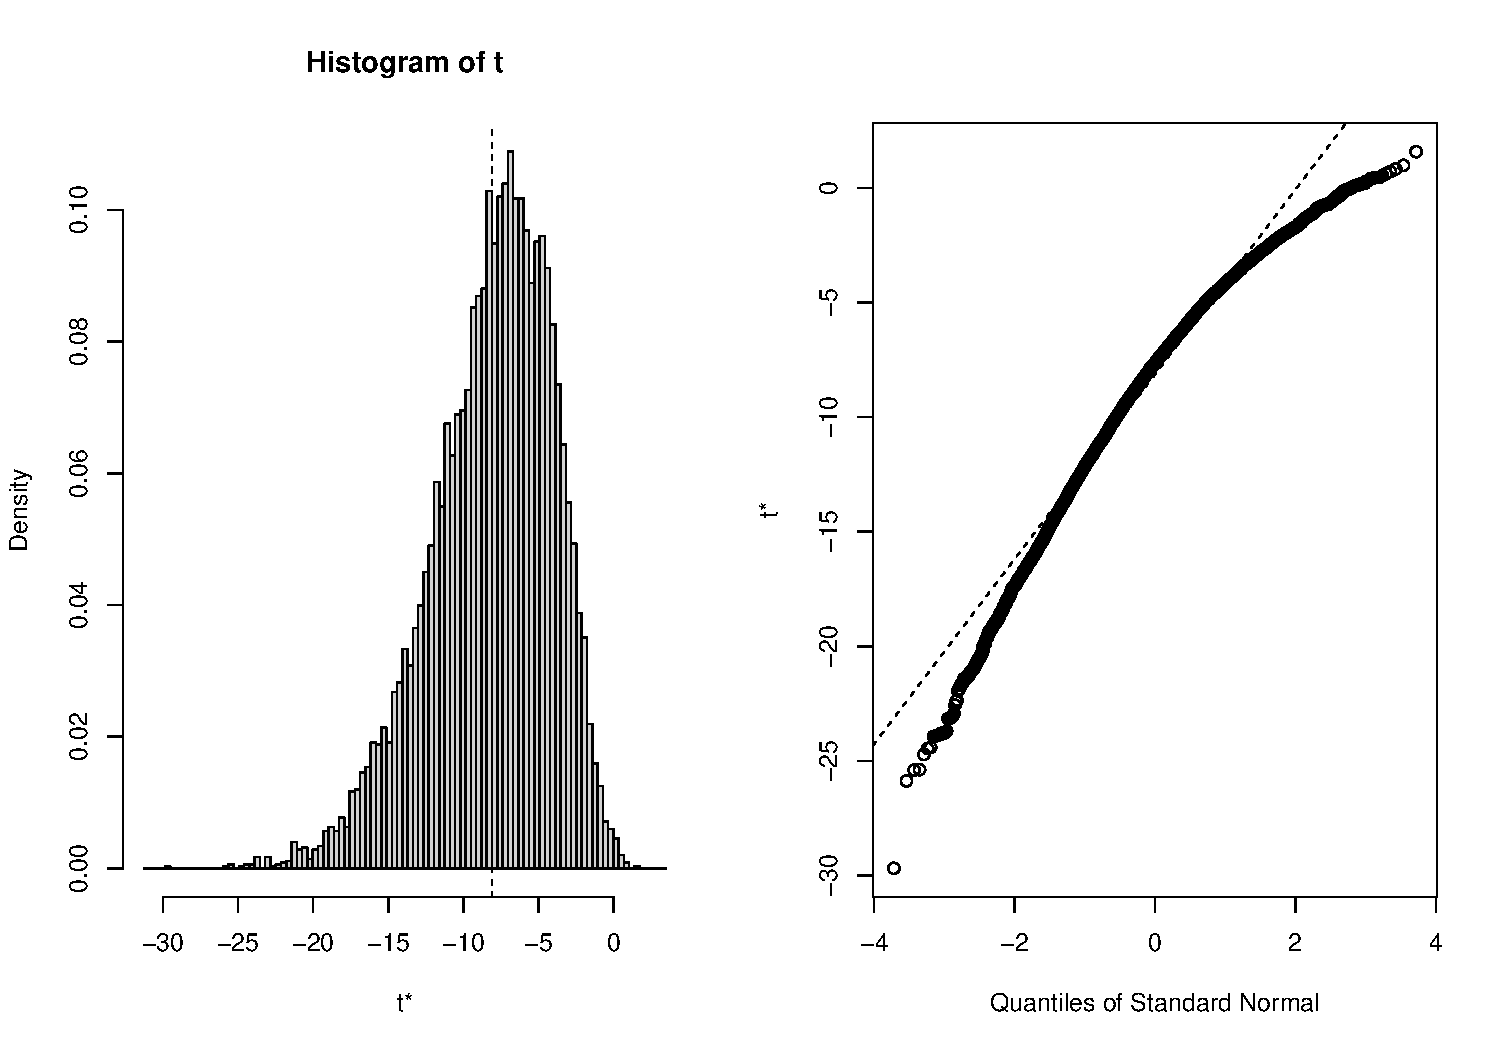
\includegraphics[width=0.8\linewidth,height=0.45\textheight]{Week11_12_13_files/figure-beamer/unnamed-chunk-34-1} \end{center}
\normalsize
\end{frame}

\begin{frame}[fragile]{Using the package boot for the difference in
means}
\protect\hypertarget{using-the-package-boot-for-the-difference-in-means-2}{}
\tiny

\begin{Shaded}
\begin{Highlighting}[]
\FunctionTok{par}\NormalTok{(}\AttributeTok{mfrow =} \FunctionTok{c}\NormalTok{(}\DecValTok{1}\NormalTok{, }\DecValTok{2}\NormalTok{))}
\FunctionTok{hist}\NormalTok{(boot.out}\SpecialCharTok{$}\NormalTok{t[,}\DecValTok{1}\NormalTok{], }\AttributeTok{col =} \StringTok{"pink"}\NormalTok{, }\AttributeTok{breaks =} \StringTok{"Scott"}\NormalTok{, }
     \AttributeTok{main =} \StringTok{""}\NormalTok{, }\AttributeTok{freq=} \ConstantTok{FALSE}\NormalTok{, }\AttributeTok{xlab =} \FunctionTok{substitute}\NormalTok{(}\FunctionTok{paste}\NormalTok{(}\FunctionTok{bar}\NormalTok{(x)[}\DecValTok{1}\NormalTok{],}\StringTok{"* {-} "}\NormalTok{, }\FunctionTok{bar}\NormalTok{(x)[}\DecValTok{2}\NormalTok{],}\StringTok{"*"}\NormalTok{)))}
\FunctionTok{lines}\NormalTok{(}\FunctionTok{density}\NormalTok{(boot.out}\SpecialCharTok{$}\NormalTok{t[,}\DecValTok{1}\NormalTok{]), }\AttributeTok{lwd =} \DecValTok{2}\NormalTok{)}
\FunctionTok{hist}\NormalTok{((boot.out}\SpecialCharTok{$}\NormalTok{t[,}\DecValTok{1}\NormalTok{] }\SpecialCharTok{{-}}\NormalTok{ boot.out}\SpecialCharTok{$}\NormalTok{t0[}\DecValTok{1}\NormalTok{])}\SpecialCharTok{/}\NormalTok{(boot.out}\SpecialCharTok{$}\NormalTok{t[,}\DecValTok{2}\NormalTok{])}\SpecialCharTok{\^{}}\NormalTok{.}\DecValTok{5}\NormalTok{, }\AttributeTok{col =} \StringTok{"pink"}\NormalTok{, }\AttributeTok{breaks =} \StringTok{"Scott"}\NormalTok{, }
     \AttributeTok{main =} \StringTok{""}\NormalTok{, }\AttributeTok{xlab =}\StringTok{"T*"}\NormalTok{, }\AttributeTok{freq=} \ConstantTok{FALSE}\NormalTok{)}
\FunctionTok{lines}\NormalTok{(}\FunctionTok{density}\NormalTok{((boot.out}\SpecialCharTok{$}\NormalTok{t[,}\DecValTok{1}\NormalTok{] }\SpecialCharTok{{-}}\NormalTok{ boot.out}\SpecialCharTok{$}\NormalTok{t0[}\DecValTok{1}\NormalTok{])}\SpecialCharTok{/}\NormalTok{(boot.out}\SpecialCharTok{$}\NormalTok{t[,}\DecValTok{2}\NormalTok{])}\SpecialCharTok{\^{}}\NormalTok{.}\DecValTok{5}\NormalTok{), }\AttributeTok{lwd =} \DecValTok{2}\NormalTok{)}
\end{Highlighting}
\end{Shaded}

\begin{center}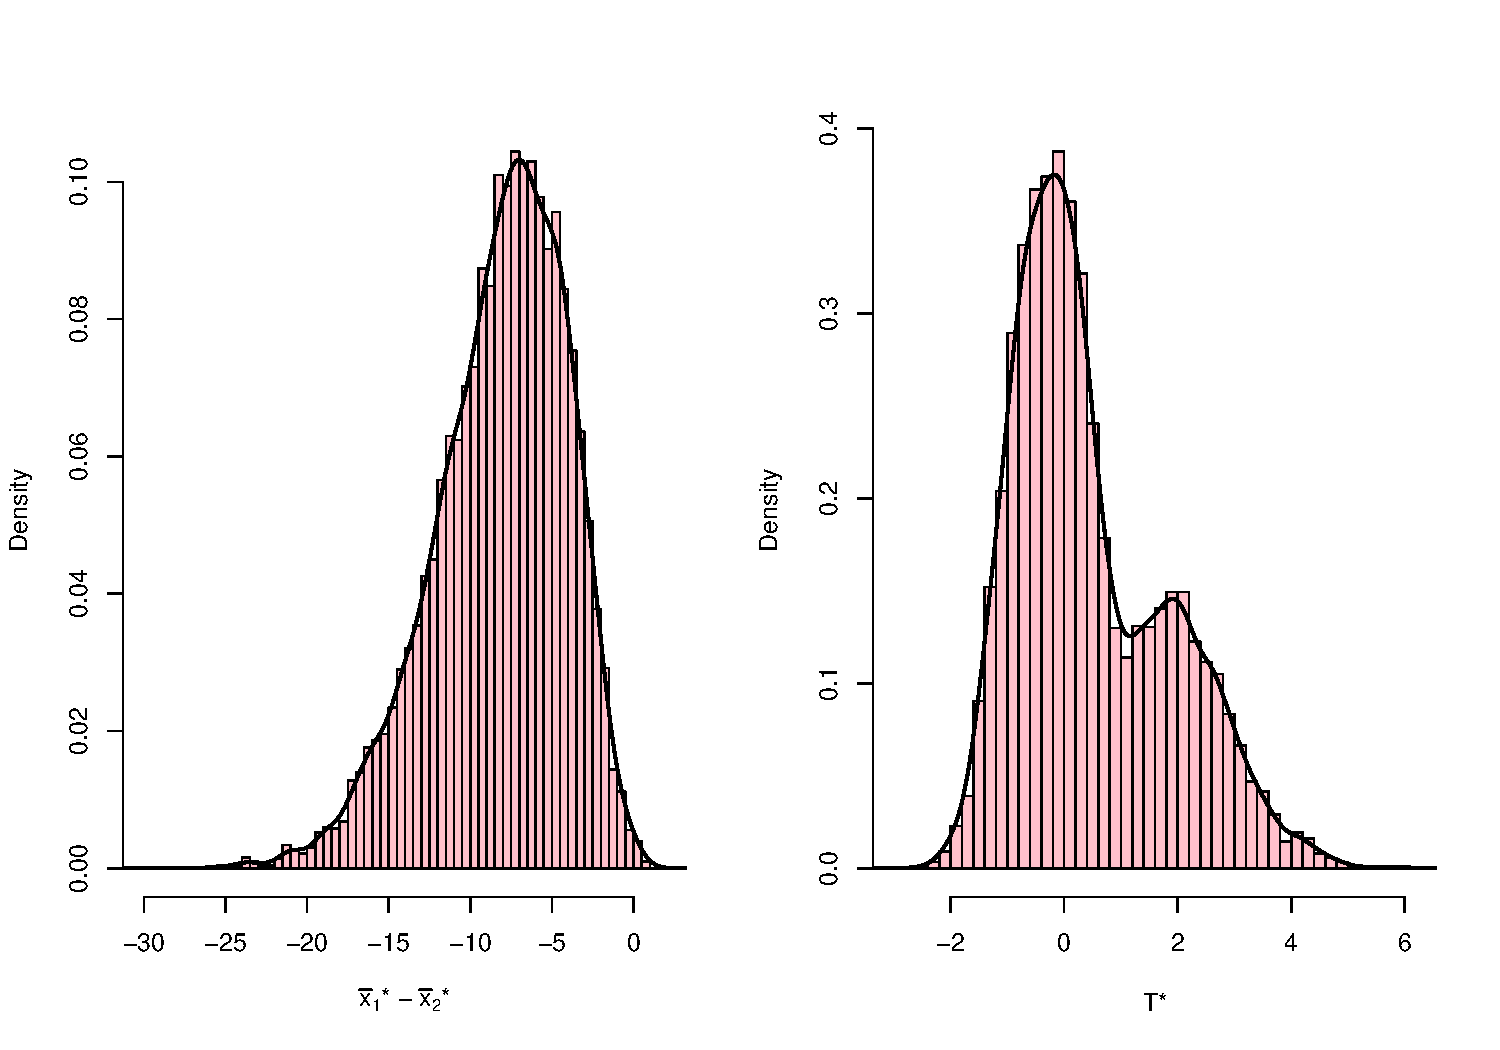
\includegraphics[width=0.8\linewidth,height=0.45\textheight]{Week11_12_13_files/figure-beamer/unnamed-chunk-35-1} \end{center}
\normalsize
\end{frame}

\begin{frame}{Comparing Bootstrap \(t\) and Formula \(t\) Confidence
Intervals}
\protect\hypertarget{comparing-bootstrap-t-and-formula-t-confidence-intervals}{}
\begin{itemize}
\item
  Where the bootstrap does differ from classical inference is in how it
  handles skewness.

  \begin{itemize}
  \tightlist
  \item
    The bootstrap percentile interval and bootstrap \(t\) interval are
    in general asymmetrical, with asymmetry depending on the sample.
  \item
    These intervals estimate the skewness of a population from the
    skewness of the sample.
  \item
    In contrast, classical \(t\) intervals assume that the population
    has no underlying skewness (skewness is 0).
  \end{itemize}
\item
  Which is preferred? Frankly, neither, but rather something in between.

  \begin{itemize}
  \tightlist
  \item
    This is an area that needs attention from statistical researchers.
  \item
    Until then, we will recommend the formula \(t\) if \(n\leq 10\), and
    the bootstrap \(t\) otherwise; the reason being in large samples, we
    should put more trust in the data, in this case, the bootstrap \(t\)
    is preferred.
  \item
    Also, the bootstrap percentile makes less of a skewness correction
    than does the bootstrap \(t\). For larger samples, the bootstrap
    \(t\) is preferred.
  \end{itemize}
\end{itemize}
\end{frame}

\hypertarget{hypothesis-testing}{%
\section{Hypothesis Testing}\label{hypothesis-testing}}

\begin{frame}{Fundamental Question of Inference}
\protect\hypertarget{fundamental-question-of-inference}{}
How does what we observed in our data compare to what would happen if
the null hypothesis were actually true and we repeated the process many
times?
\end{frame}

\begin{frame}{Hypothesis Testing}
\protect\hypertarget{hypothesis-testing-1}{}
\begin{itemize}
\item
  Now that we've studied confidence intervals, let's study another
  commonly used method for statistical inference: \textbf{hypothesis
  testing}.
\item
  Hypothesis tests allow us to take a sample of data from a population
  and infer about the plausibility of competing hypotheses.
\item
  The good news is we've already covered many of the necessary concepts
  to understand hypothesis testing.

  \begin{itemize}
  \tightlist
  \item
    We will expand further on these ideas and provide a general
    framework for understanding hypothesis tests.
  \end{itemize}
\end{itemize}
\end{frame}

\begin{frame}[fragile]{Needed packages}
\protect\hypertarget{needed-packages-1}{}
Let's load all the packages needed for this chapter

\small

\begin{Shaded}
\begin{Highlighting}[]
\FunctionTok{library}\NormalTok{(tidyverse)}
\FunctionTok{library}\NormalTok{(infer)}
\FunctionTok{library}\NormalTok{(moderndive)}
\FunctionTok{library}\NormalTok{(nycflights13)}
\FunctionTok{library}\NormalTok{(ggplot2movies)}
\end{Highlighting}
\end{Shaded}

\normalsize
\end{frame}

\begin{frame}{Promotions activity}
\protect\hypertarget{promotions-activity}{}
Let's start with an activity studying the effect of gender on promotions
at a bank.

\begin{itemize}
\item
  Say you are working at a bank in the 1970s and you are submitting your
  résumé to apply for a promotion.
\item
  Will your gender affect your chances of getting promoted?
\item
  To answer this question, we'll focus on data from a study published in
  the Journal of Applied Psychology in 1974.
\end{itemize}
\end{frame}

\begin{frame}{Promotions activity}
\protect\hypertarget{promotions-activity-1}{}
To begin the study, 48 bank supervisors were asked to assume the role of
a hypothetical director of a bank with multiple branches.

\begin{itemize}
\item
  Every one of the bank supervisors was given a résumé and asked whether
  or not the candidate on the résumé was fit to be promoted to a new
  position in one of their branches.
\item
  However, each of these 48 résumés were identical in all respects
  except one: the name of the applicant at the top of the résumé.
\item
  Of the supervisors,

  \begin{itemize}
  \tightlist
  \item
    24 were randomly given résumés with stereotypically ``male'' names,
    while - 24 of the supervisors were randomly given résumés with
    stereotypically ``female'' names.
  \end{itemize}
\item
  Since only gender varied from résumé to résumé, researchers could
  isolate the effect of this variable in promotion rates.
\end{itemize}
\end{frame}

\begin{frame}[fragile]{Promotions activity}
\protect\hypertarget{promotions-activity-2}{}
The \texttt{moderndive} package contains the data on the 48 applicants
in the \texttt{promotions} data frame.

\tiny

\begin{Shaded}
\begin{Highlighting}[]
\NormalTok{promotions }\SpecialCharTok{\%\textgreater{}\%} 
  \FunctionTok{sample\_n}\NormalTok{(}\AttributeTok{size =} \DecValTok{10}\NormalTok{) }\SpecialCharTok{\%\textgreater{}\%} 
  \FunctionTok{arrange}\NormalTok{(id)}
\end{Highlighting}
\end{Shaded}

\begin{verbatim}
# A tibble: 10 x 3
      id decision gender
   <int> <fct>    <fct> 
 1     4 promoted male  
 2     7 promoted male  
 3    14 promoted male  
 4    15 promoted male  
 5    16 promoted male  
 6    26 promoted female
 7    30 promoted female
 8    33 promoted female
 9    41 not      female
10    45 not      female
\end{verbatim}

\normalsize
\end{frame}

\begin{frame}[fragile]{Promotions activity}
\protect\hypertarget{promotions-activity-3}{}
Let's perform an exploratory data analysis of the relationship between
the two categorical variables \texttt{decision} and \texttt{gender}.

\tiny

\begin{Shaded}
\begin{Highlighting}[]
\FunctionTok{ggplot}\NormalTok{(promotions, }\FunctionTok{aes}\NormalTok{(}\AttributeTok{x =}\NormalTok{ gender, }\AttributeTok{fill =}\NormalTok{ decision)) }\SpecialCharTok{+}
  \FunctionTok{geom\_bar}\NormalTok{() }\SpecialCharTok{+}
  \FunctionTok{labs}\NormalTok{(}\AttributeTok{x =} \StringTok{"Gender of name on résumé"}\NormalTok{)}
\end{Highlighting}
\end{Shaded}

\begin{center}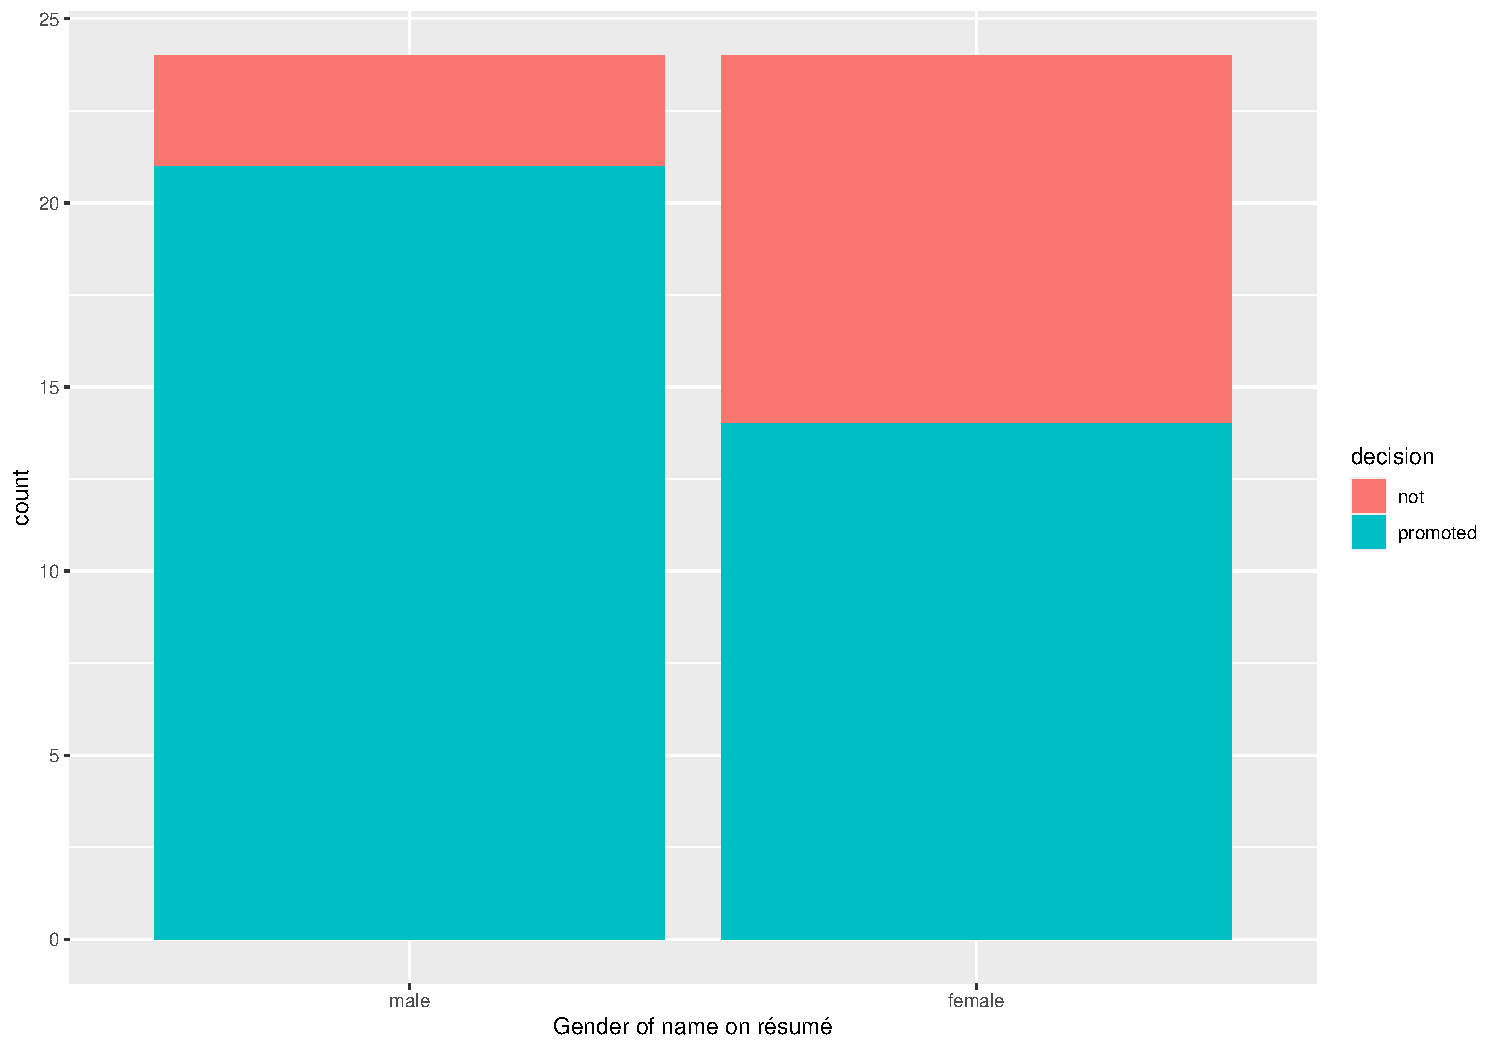
\includegraphics[width=0.7\linewidth,height=0.45\textheight]{Week11_12_13_files/figure-beamer/unnamed-chunk-38-1} \end{center}
\normalsize

Observe that it appears that résumés with female names were much less
likely to be accepted for promotion.
\end{frame}

\begin{frame}[fragile]{Promotions activity}
\protect\hypertarget{promotions-activity-4}{}
Let's quantify these promotion rates

\tiny

\begin{Shaded}
\begin{Highlighting}[]
\NormalTok{promotions }\SpecialCharTok{\%\textgreater{}\%} 
  \FunctionTok{group\_by}\NormalTok{(gender, decision) }\SpecialCharTok{\%\textgreater{}\%} 
  \FunctionTok{tally}\NormalTok{()}
\end{Highlighting}
\end{Shaded}

\begin{verbatim}
# A tibble: 4 x 3
# Groups:   gender [2]
  gender decision     n
  <fct>  <fct>    <int>
1 male   not          3
2 male   promoted    21
3 female not         10
4 female promoted    14
\end{verbatim}

\normalsize

\begin{itemize}
\item
  So of the 24 résumés

  \begin{itemize}
  \tightlist
  \item
    with male names: \(21/24=0.875=87.5\%\) were selected for promotion.
  \item
    with female names: \(14/24=0.583=58.3\%\) were selected for
    promotion.
  \end{itemize}
\end{itemize}

Résumés with male names were selected for promotion at a rate
\(0.875 -0.583 = 0.292 = 29.2\%\) higher than résumés with female names.
\end{frame}

\begin{frame}{Promotions activity}
\protect\hypertarget{promotions-activity-5}{}
The question is, however, does this provide conclusive evidence that
there is gender discrimination in promotions at banks?

\begin{itemize}
\item
  Could a difference in promotion rates of \(29.2\%\) still occur by
  chance, even in a hypothetical world where no gender-based
  discrimination existed?
\item
  In other words, what is the role of sampling variation in this
  hypothesized world?
\item
  To answer this question, we'll again rely on a computer to run
  simulations.
\end{itemize}
\end{frame}

\begin{frame}[fragile]{Promotions activity: Shuffling once}
\protect\hypertarget{promotions-activity-shuffling-once}{}
First, try to imagine a hypothetical universe where no gender
discrimination in promotions existed.

\begin{itemize}
\item
  In such a hypothetical universe, the gender of an applicant would have
  no bearing on their chances of promotion
\item
  Bringing things back to our \texttt{promotions} data frame, the
  \texttt{gender} variable would thus be an irrelevant label.
\item
  If these \texttt{gender} labels were irrelevant, then we could
  randomly reassign them by ``shuffling'' them to no consequence!
\end{itemize}
\end{frame}

\begin{frame}[fragile]{Promotions activity: Shuffling once}
\protect\hypertarget{promotions-activity-shuffling-once-1}{}
\begin{itemize}
\item
  To illustrate this idea, let's narrow our focus to 6 arbitrarily
  chosen résumés of the 48.

  \begin{itemize}
  \item
    The decision column shows that 3 résumés resulted in promotion while
    3 didn't.
  \item
    The gender column shows what the original gender of the résumé name
    was.
  \item
    The \texttt{shuffled\_gender} shows a random ``shuffle'' values of
    gender.
  \end{itemize}
\end{itemize}

\begin{center}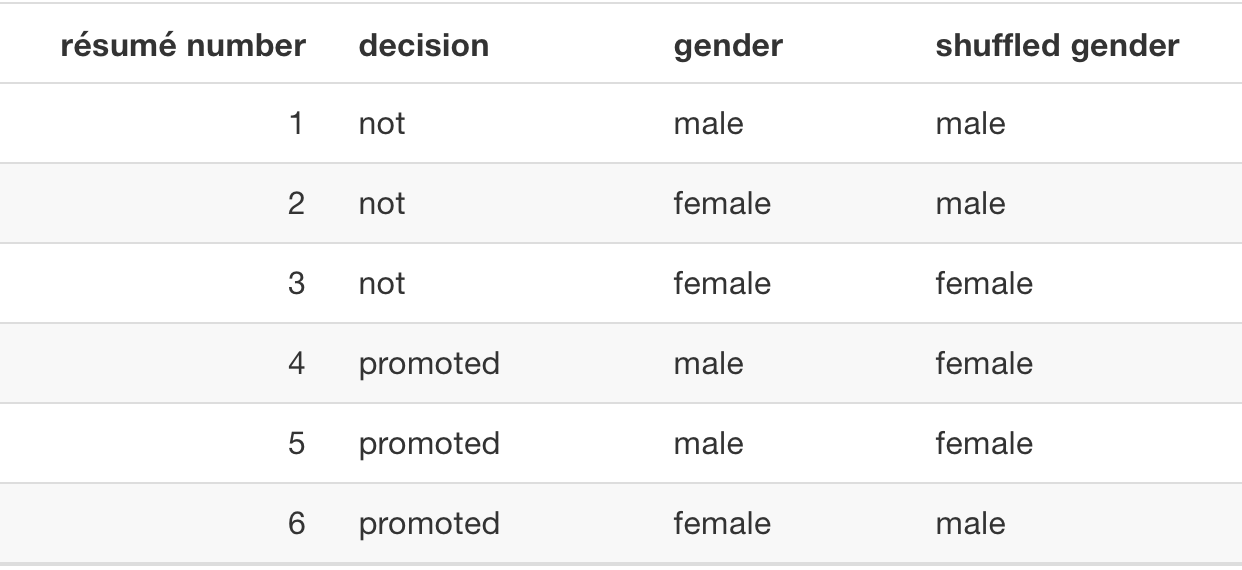
\includegraphics[width=0.7\linewidth,height=0.4\textheight]{week12_1} \end{center}
\end{frame}

\begin{frame}{Promotions activity: Shuffling once}
\protect\hypertarget{promotions-activity-shuffling-once-2}{}
\begin{itemize}
\item
  Again, such random shuffling of the gender label only makes sense in
  our hypothesized universe of no gender discrimination.
\item
  How could we extend this shuffling of the gender variable to all 48
  résumés by hand?
\item
  One way would be by using a standard deck of 52 playing cards,
\end{itemize}

\begin{center}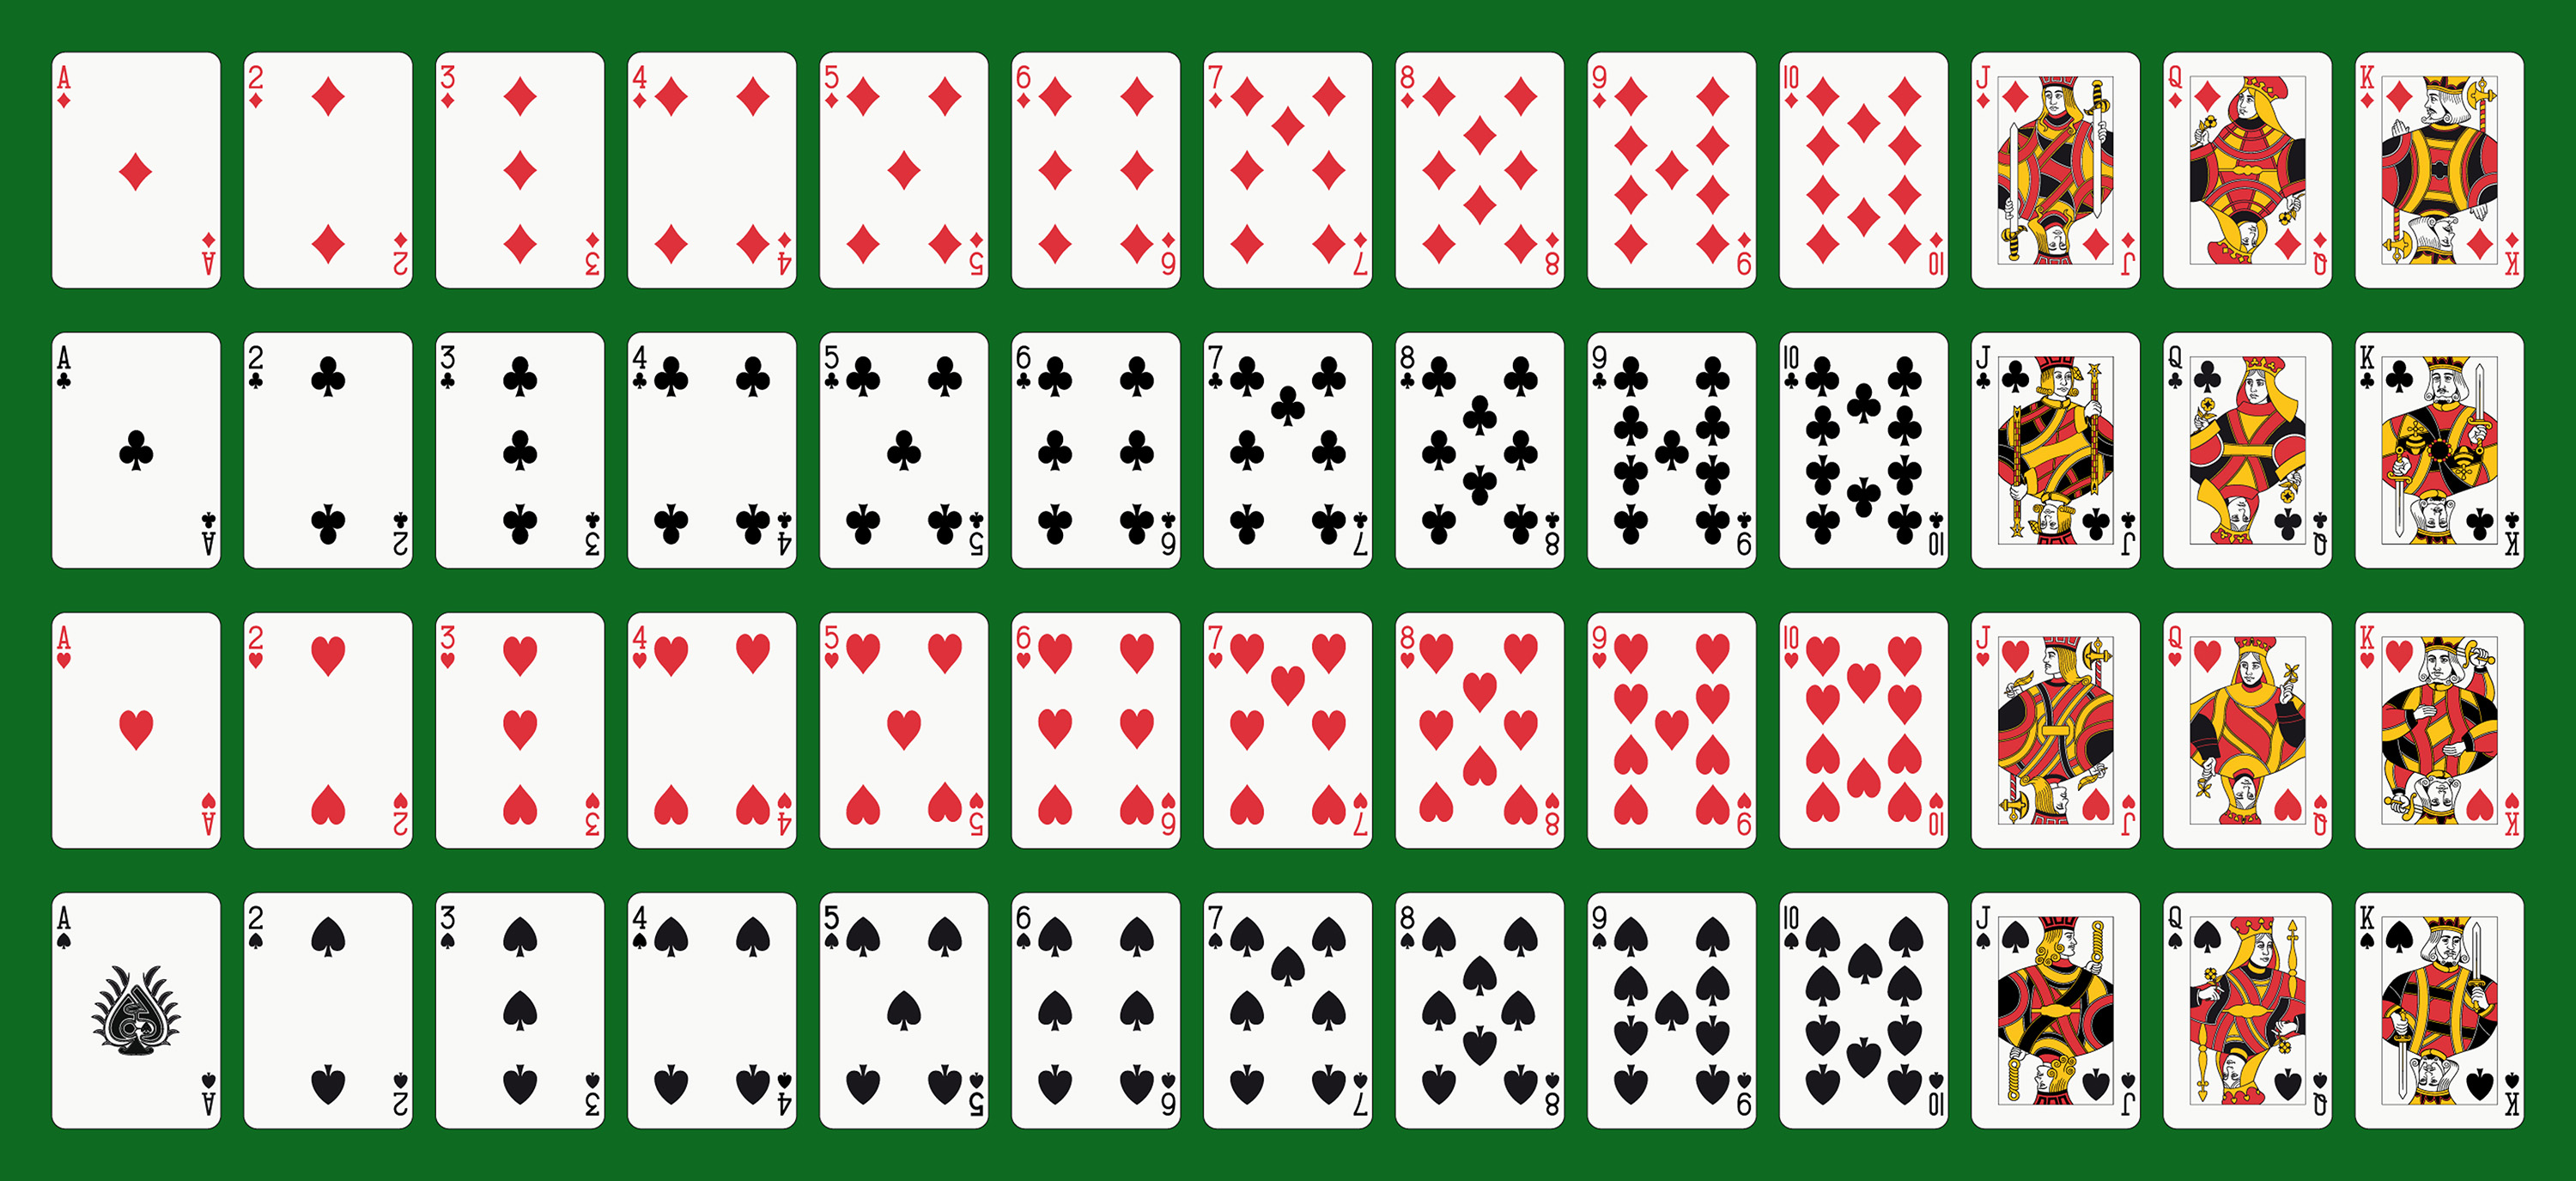
\includegraphics[width=0.7\linewidth,height=0.4\textheight]{week12_2} \end{center}

\begin{itemize}
\tightlist
\item
  By removing two red cards and two black cards, we would end up with 24
  red cards and 24 black cards.
\end{itemize}
\end{frame}

\begin{frame}{Promotions activity: Shuffling once}
\protect\hypertarget{promotions-activity-shuffling-once-3}{}
\begin{itemize}
\tightlist
\item
  After shuffling these 48 cards as seen below.
\end{itemize}

\begin{center}
\includegraphics[width=0.7\linewidth,height=0.4\textheight]{week12_3} \end{center}

\begin{itemize}
\tightlist
\item
  we can flip the cards over one-by-one, assigning ``male'' for each red
  card and ``female'' for each black card.
\end{itemize}
\end{frame}

\begin{frame}[fragile]{Promotions activity: Shuffling once}
\protect\hypertarget{promotions-activity-shuffling-once-4}{}
We have one such shuffling in the \texttt{promotions\_shuffled} data
frame of the \texttt{moderndive} package:

\tiny

\begin{Shaded}
\begin{Highlighting}[]
\FunctionTok{ggplot}\NormalTok{(promotions\_shuffled, }
       \FunctionTok{aes}\NormalTok{(}\AttributeTok{x =}\NormalTok{ gender, }\AttributeTok{fill =}\NormalTok{ decision)) }\SpecialCharTok{+}
  \FunctionTok{geom\_bar}\NormalTok{() }\SpecialCharTok{+} 
  \FunctionTok{labs}\NormalTok{(}\AttributeTok{x =} \StringTok{"Gender of résumé name"}\NormalTok{)}
\end{Highlighting}
\end{Shaded}

\begin{center}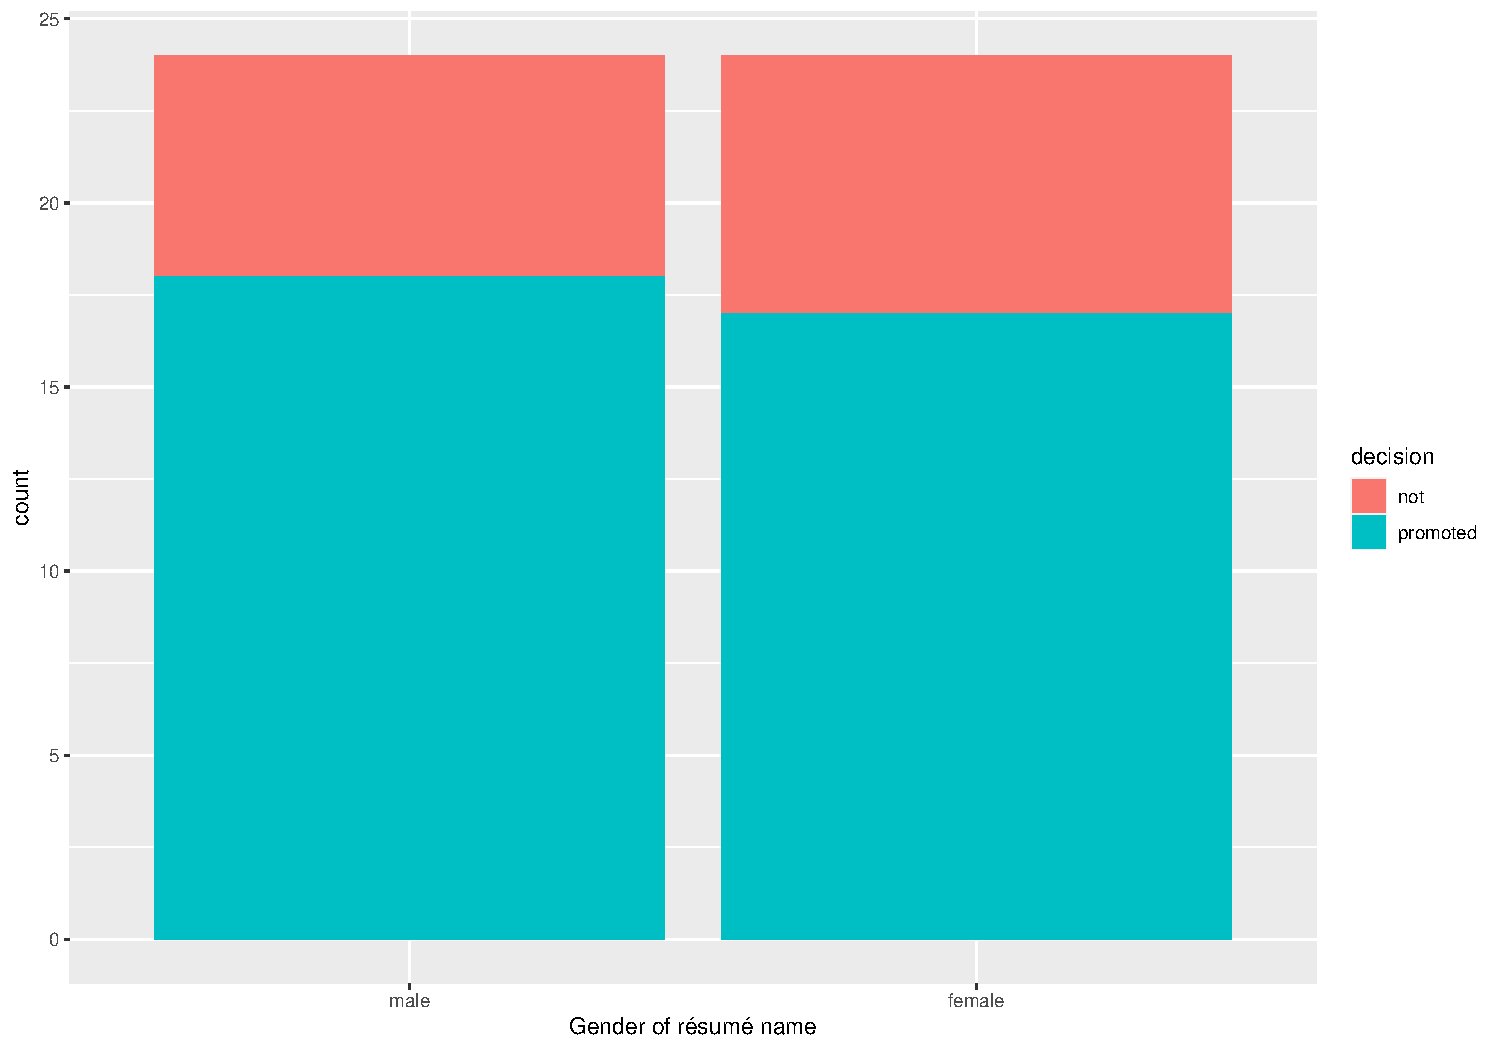
\includegraphics[width=0.7\linewidth,height=0.4\textheight]{Week11_12_13_files/figure-beamer/unnamed-chunk-43-1} \end{center}
\normalsize

It appears the difference in ``male names'' versus ``female names''
promotion rates is now different.
\end{frame}

\begin{frame}[fragile]{Promotions activity: Shuffling once}
\protect\hypertarget{promotions-activity-shuffling-once-5}{}
Let's also compute the proportion of résumés accepted for promotion for
each group:

\tiny

\begin{Shaded}
\begin{Highlighting}[]
\NormalTok{promotions\_shuffled }\SpecialCharTok{\%\textgreater{}\%} 
  \FunctionTok{group\_by}\NormalTok{(gender, decision) }\SpecialCharTok{\%\textgreater{}\%} 
  \FunctionTok{tally}\NormalTok{() }\CommentTok{\# Same as summarize(n = n())}
\end{Highlighting}
\end{Shaded}

\begin{verbatim}
# A tibble: 4 x 3
# Groups:   gender [2]
  gender decision     n
  <fct>  <fct>    <int>
1 male   not          6
2 male   promoted    18
3 female not          7
4 female promoted    17
\end{verbatim}

\normalsize

\begin{itemize}
\item
  So in this hypothetical universe of no discrimination:

  \begin{itemize}
  \tightlist
  \item
    \(18/24=0.75=75\%\) of ``male'' résumés were selected for promotion.
  \item
    \(17/24=0.708=70.8\%\) of ``male'' résumés were selected for
    promotion.
  \end{itemize}
\end{itemize}

Résumés with male names were selected for promotion at a rate
\(0.75 -0.708 = 0.042 = 4.2\%\) higher than résumés with female names.
\end{frame}

\begin{frame}{Promotions activity: Shuffling 16 times}
\protect\hypertarget{promotions-activity-shuffling-16-times}{}
\begin{itemize}
\item
  We recruited 16 groups of our friends to repeat this shuffling
  exercise.
\item
  The distribution of the difference in promotion rates in shown below.
\item
  The observed difference in promotion rate that occurred in real life
  (\(0.292 = 29.2\%\)) is depicted with a vertical red line.
\end{itemize}

\begin{center}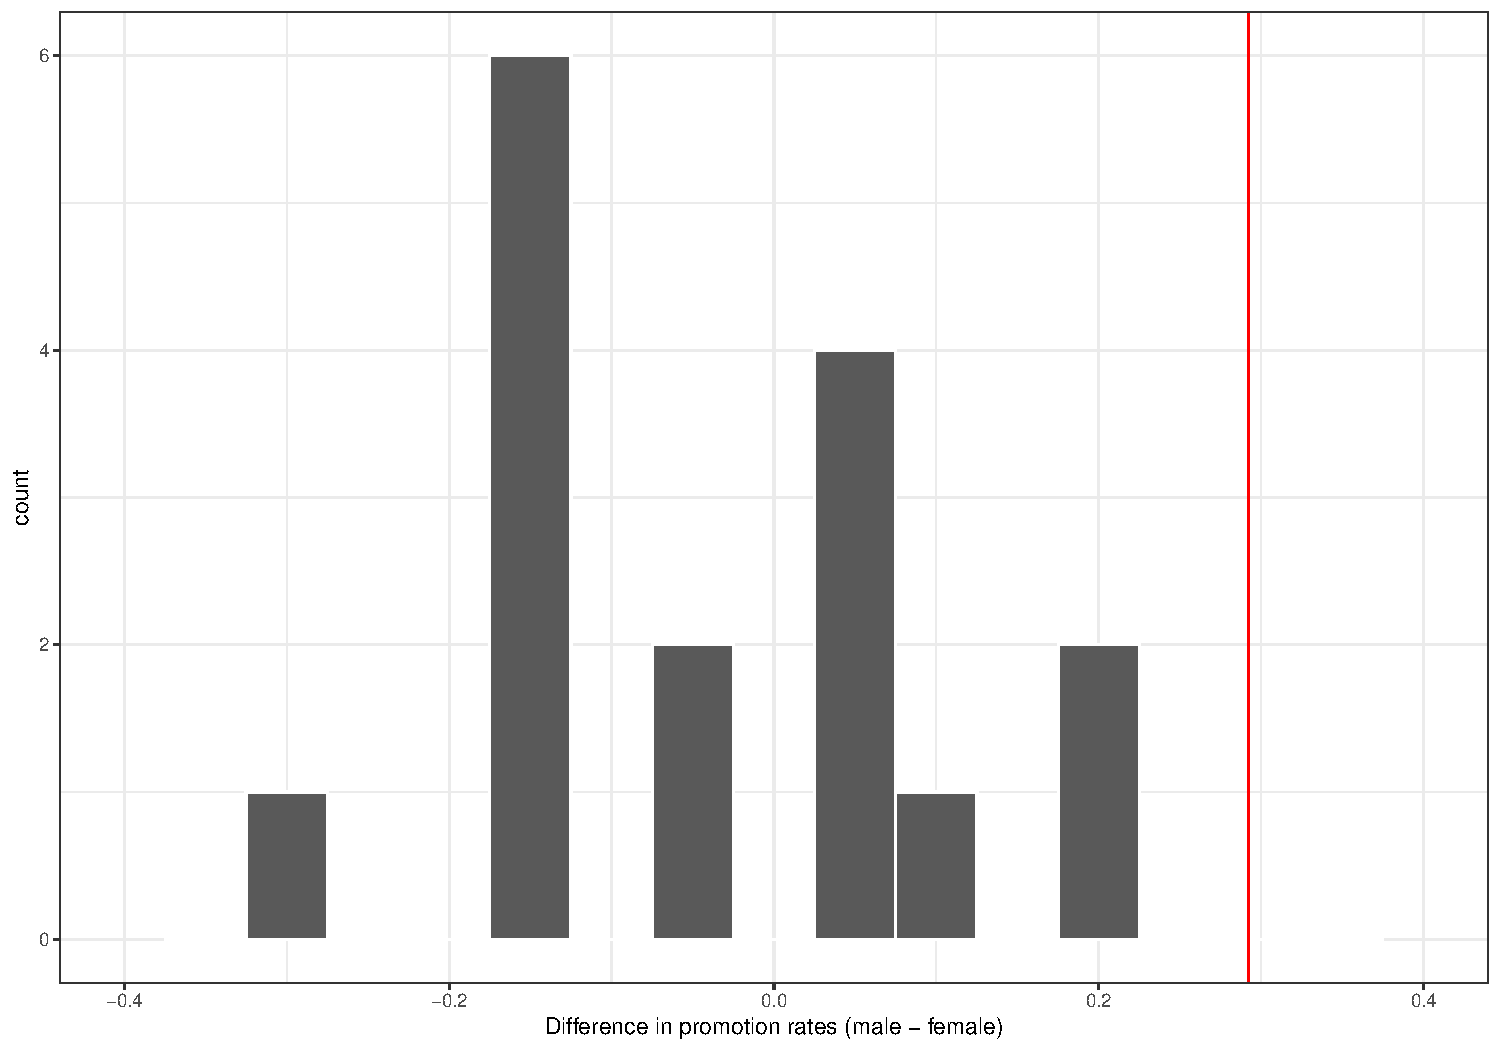
\includegraphics[width=0.7\linewidth,height=0.4\textheight]{Week11_12_13_files/figure-beamer/unnamed-chunk-45-1} \end{center}
\end{frame}

\begin{frame}{Promotions activity: Shuffling 16 times}
\protect\hypertarget{promotions-activity-shuffling-16-times-1}{}
Things to note:

\begin{itemize}
\item
  Observe first that the histogram is roughly centered at 0 (actual mean
  is -0.0260417).

  \begin{itemize}
  \tightlist
  \item
    Saying that the difference in promotion rates is 0 is equivalent to
    saying that both genders had the same promotion rate.
  \item
    In other words, the center of these 16 values is consistent with
    what we would expect in our hypothesized universe of no gender
    discrimination.
  \end{itemize}
\item
  However, while the values are centered at 0, there is variation about
  0.

  \begin{itemize}
  \tightlist
  \item
    Even in a hypothesized universe of no gender discrimination, you
    will still likely observe small differences in promotion rates
    because of chance \textbf{sampling variation}.
  \item
    Looking at the histogram, such differences could even be as extreme
    as -0.2916667 or 0.2083333.
  \end{itemize}
\end{itemize}
\end{frame}

\begin{frame}{Fundamental Question of Inference}
\protect\hypertarget{fundamental-question-of-inference-1}{}
\begin{itemize}
\item
  Ask yourself:

  \begin{itemize}
  \item
    In a hypothesized world of no gender discrimination, how likely
    would it be that we observe this difference \((0.292 = 29.2\%)\)?
  \item
    What do these results say about our hypothesized universe of no
    gender discrimination?
  \end{itemize}
\end{itemize}
\end{frame}

\begin{frame}{What did we just do?}
\protect\hypertarget{what-did-we-just-do}{}
What we just demonstrated in this activity is the statistical procedure
known as \textbf{hypothesis testing} using a \textbf{permutation test}
also referred to as \textbf{randomization test}.

\begin{itemize}
\item
  The term ``permutation'' is the mathematical term for ``shuffling'':
  taking a series of values and reordering them randomly, as you did
  with the playing cards.
\item
  In fact, \textbf{permutations} are another form of
  \textbf{resampling}, like the bootstrap method you performed earlier.

  \begin{itemize}
  \tightlist
  \item
    The bootstrap method involves resampling \textbf{with} replacement.
  \item
    The permutation method involves resampling \textbf{without}
    replacement.
  \end{itemize}
\end{itemize}
\end{frame}

\begin{frame}[fragile]{What did we just do?}
\protect\hypertarget{what-did-we-just-do-1}{}
In our previous example, we tested the validity of the hypothesized
universe of no gender discrimination.

\tiny

\begin{Shaded}
\begin{Highlighting}[]
\FunctionTok{set.seed}\NormalTok{(}\DecValTok{37}\NormalTok{)}
\NormalTok{promotions }\SpecialCharTok{\%\textgreater{}\%} 
  \FunctionTok{specify}\NormalTok{(}\AttributeTok{formula =}\NormalTok{ decision }\SpecialCharTok{\textasciitilde{}}\NormalTok{ gender, }\AttributeTok{success =} \StringTok{"promoted"}\NormalTok{) }\SpecialCharTok{\%\textgreater{}\%} 
  \FunctionTok{hypothesize}\NormalTok{(}\AttributeTok{null =} \StringTok{"independence"}\NormalTok{) }\SpecialCharTok{\%\textgreater{}\%} 
  \FunctionTok{generate}\NormalTok{(}\AttributeTok{reps =} \DecValTok{1000}\NormalTok{, }\AttributeTok{type =} \StringTok{"permute"}\NormalTok{) }\SpecialCharTok{\%\textgreater{}\%} 
  \FunctionTok{calculate}\NormalTok{(}\AttributeTok{stat =} \StringTok{"diff in props"}\NormalTok{, }\AttributeTok{order =} \FunctionTok{c}\NormalTok{(}\StringTok{"male"}\NormalTok{, }\StringTok{"female"}\NormalTok{)) }\OtherTok{{-}\textgreater{}}\NormalTok{ null\_distribution}
\FunctionTok{get\_pvalue}\NormalTok{(null\_distribution, }\AttributeTok{obs\_stat=}\NormalTok{ .}\DecValTok{292}\NormalTok{, }\AttributeTok{direction =} \StringTok{"right"}\NormalTok{) }\OtherTok{{-}\textgreater{}}\NormalTok{ pv}
\NormalTok{pv}
\end{Highlighting}
\end{Shaded}

\begin{verbatim}
# A tibble: 1 x 1
  p_value
    <dbl>
1   0.002
\end{verbatim}

\normalsize

\begin{itemize}
\item
  The evidence contained in our observed sample of 48 résumés was
  somewhat inconsistent with our hypothesized universe. In the
  simulation above only 2 of the 1000 permutations yielded a difference
  as extreme or more than the observed difference of 0.292.
\item
  Thus, we would be inclined to \textbf{reject} this hypothesized
  universe and declare that the evidence suggests there is gender
  discrimination.
\end{itemize}
\end{frame}

\hypertarget{understanding-hypothesis-tests}{%
\section{Understanding hypothesis
tests}\label{understanding-hypothesis-tests}}

\begin{frame}{Understanding hypothesis tests}
\protect\hypertarget{understanding-hypothesis-tests-1}{}
Terminology, notation, and definitions related to hypothesis testing.

\begin{itemize}
\item
  First, a \textbf{hypothesis} is a statement about the value of an
  unknown population parameter.

  \begin{itemize}
  \tightlist
  \item
    In our résumé activity, our population parameter of interest is the
    difference in population proportions \(p_m - p_f\).
  \item
    Hypothesis tests can involve any of the population parameters below:
  \end{itemize}
\end{itemize}

\begin{center}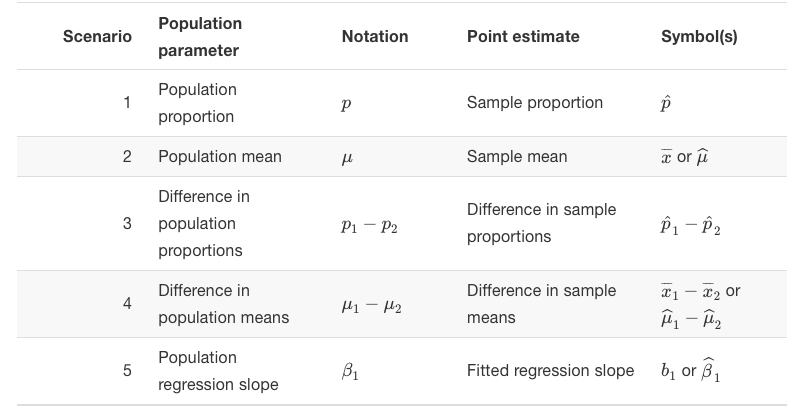
\includegraphics[width=0.7\linewidth,height=0.5\textheight]{week12_5} \end{center}
\end{frame}

\begin{frame}{Understanding hypothesis tests}
\protect\hypertarget{understanding-hypothesis-tests-2}{}
Second, a hypothesis test consists of a test between two competing
hypotheses:

\begin{enumerate}
[(1)]
\item
  a null hypothesis \(H_0\) (pronounced ``H-naught'')

  \begin{itemize}
  \tightlist
  \item
    Generally the null hypothesis is a claim that there is ``no effect''
    or ``no difference of interest.''
  \end{itemize}
\item
  versus an alternative hypothesis \(H_A\) (also denoted \(H_1\)).

  \begin{itemize}
  \tightlist
  \item
    Generally the alternative hypothesis is the claim the experimenter
    or researcher wants to establish or find evidence to support.
  \item
    It is viewed as a ``challenger'' hypothesis to the null hypothesis
    \(H_0\).
  \end{itemize}
\end{enumerate}
\end{frame}

\begin{frame}{Understanding hypothesis tests}
\protect\hypertarget{understanding-hypothesis-tests-3}{}
In our résumé activity, an appropriate hypothesis test would be:

\[\begin{array}{ll}
&H_0: \text{men and women are promoted at the same rate}\\
vs&H_A: \text{men are promoted at a higher rate than women}
\end{array}\]

\begin{itemize}
\item
  Note that:

  \begin{itemize}
  \tightlist
  \item
    \(H_0\) states there is no difference in promotion rate.
  \item
    \(H_A\) states men are promoted at a higher rate than women, a
    subjective choice reflecting a prior suspicion we have that this is
    the case.
  \end{itemize}
\item
  We call such alternative hypotheses \textbf{one-sided alternatives}.
\item
  If someone else however does not share such suspicions and only wants
  to investigate that there is a difference, whether higher or lower,
  they would set what is known as a \textbf{two-sided alternative}.
\end{itemize}
\end{frame}

\begin{frame}{Understanding hypothesis tests}
\protect\hypertarget{understanding-hypothesis-tests-4}{}
We can write our hypothesis test using the mathematical notation as:

\[\begin{array}{ll}
&H_0: p_m-p_f=0\\
vs&H_A: p_m-p_f>0
\end{array}\] Here \(H_A\) is one sided. Had we opted for a two-sided
alternative, we would have written

\[\begin{array}{ll}
&H_0: p_m-p_f=0\\
vs&H_A: p_m-p_f\neq 0
\end{array}\]
\end{frame}

\begin{frame}{Understanding hypothesis tests}
\protect\hypertarget{understanding-hypothesis-tests-5}{}
\begin{itemize}
\item
  Third, a \textbf{test statistic} is a point estimate/sample statistic
  used for hypothesis testing.

  \begin{itemize}
  \tightlist
  \item
    Note that a sample statistic is merely a summary statistic based on
    a sample.
  \item
    Here, the sample resulted in \(n_m=24\) résumés with male names and
    the \(n_f\) résumés with female names.
  \item
    Hence, the point estimate of interest is the difference in sample
    proportions \(\hat{p}_m-\hat{p}_f\).
  \end{itemize}
\item
  Fourth, the \textbf{observed test statistic} is the value of the test
  statistic that we observed in real life.

  \begin{itemize}
  \tightlist
  \item
    In our case, \(\hat{p}_m-\hat{p}_f=0.875-0.583=29.2\%\) in favor of
    résumés with male names.
  \end{itemize}
\end{itemize}
\end{frame}

\begin{frame}{Understanding hypothesis tests}
\protect\hypertarget{understanding-hypothesis-tests-6}{}
Fifth, the \textbf{null distribution} is the sampling distribution of
the test statistic assuming the null hypothesis \(H_0\) is true.

\begin{itemize}
\item
  Let's unpack it slowly.

  \begin{itemize}
  \tightlist
  \item
    The key to understanding the null distribution is that the null
    hypothesis \(H_0\) is assumed to be true.
  \item
    In our case, this corresponds to our hypothesized universe of no
    gender discrimination in promotion rates.
  \end{itemize}
\item
  Assuming the null hypothesis \(H_0\), how does the test statistic vary
  due to sampling variation?

  \begin{itemize}
  \tightlist
  \item
    In our case, we examine the sampling distribution of the difference
    in sample proportions \(\hat{p}_m-\hat{p}_f\).
  \item
    Recall that distributions displaying how point estimates vary due to
    sampling variation are called \emph{sampling distributions}.
  \item
    The null distribution is the sampling distribution assuming the null
    hypothesis \(H_0\) is true.
  \end{itemize}
\end{itemize}
\end{frame}

\begin{frame}{Understanding hypothesis tests}
\protect\hypertarget{understanding-hypothesis-tests-7}{}
The null distribution from 1000 permutations is given below

\begin{center}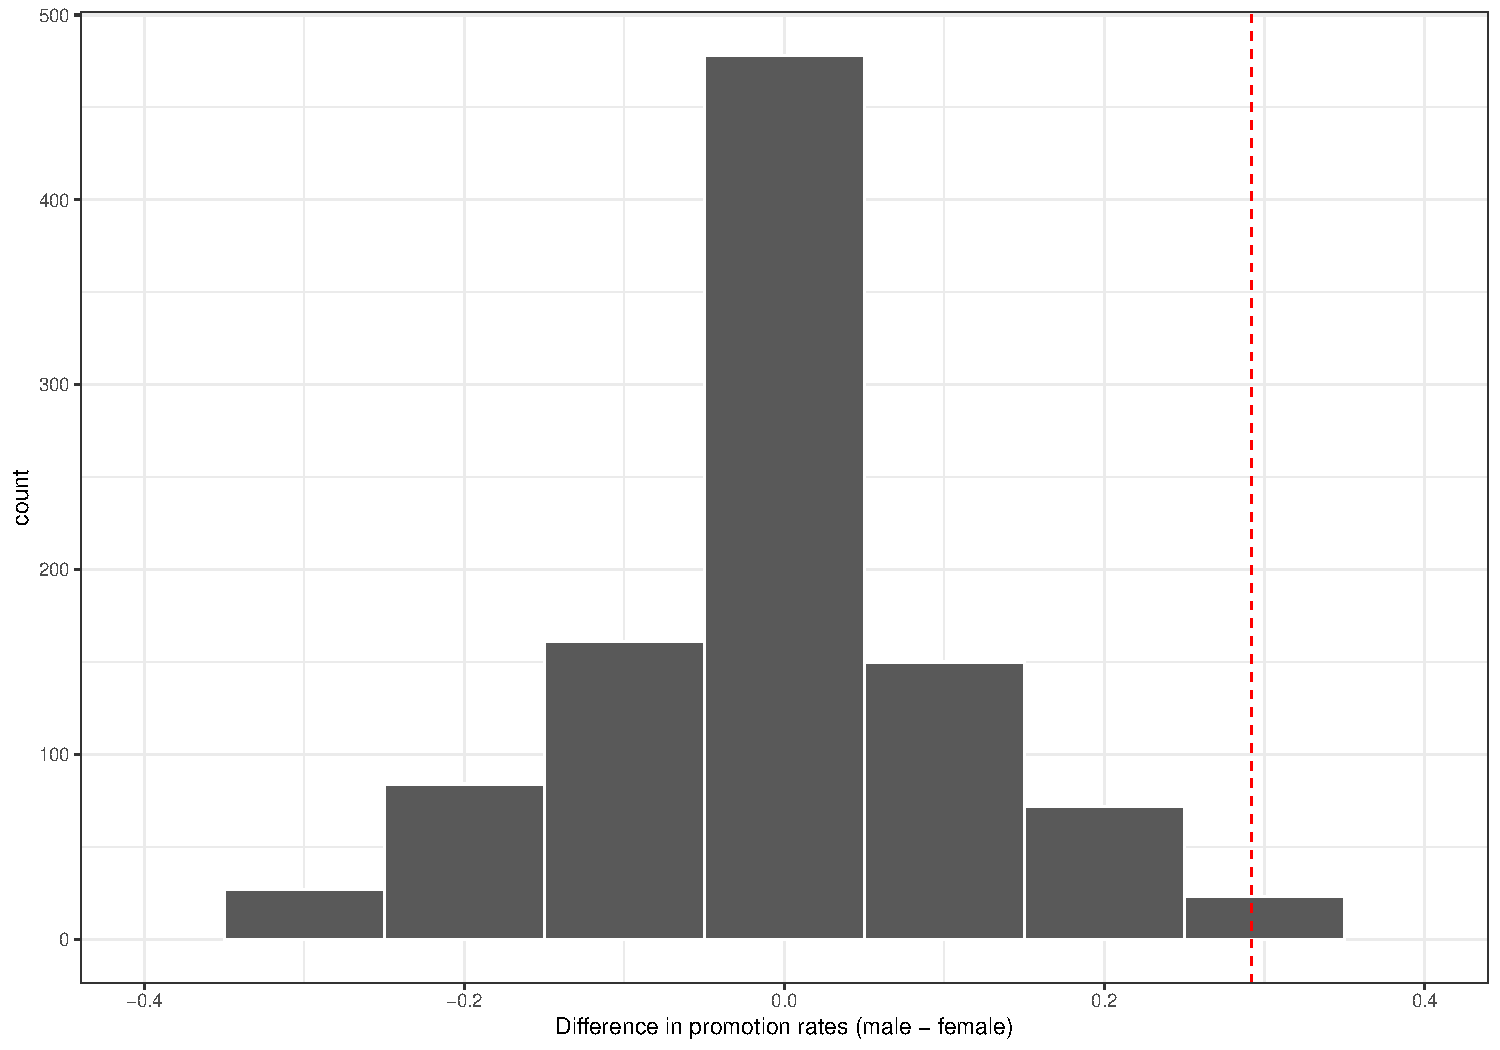
\includegraphics[width=0.6\linewidth,height=0.4\textheight]{Week11_12_13_files/figure-beamer/unnamed-chunk-48-1} \end{center}
\end{frame}

\begin{frame}{Understanding hypothesis tests}
\protect\hypertarget{understanding-hypothesis-tests-8}{}
\begin{itemize}
\item
  Sixth, the \textbf{p-value} is the probability of obtaining a test
  statistic just as extreme or more extreme than the observed test
  statistic assuming the null hypothesis \(H_0\) is true.

  \begin{itemize}
  \tightlist
  \item
    You can think of the p-value as a quantification of ``surprise'':
    assuming \(H_0\) is true, how surprised are we with what we
    observed?
  \item
    In our case, 2 times out of 1000, we obtained a difference in
    proportions greater than or equal to the observed difference of
    0.292 = 29.2\%.
  \item
    A very rare outcome if in fact the nulll hypothesis is true!
  \end{itemize}
\item
  Given the rarity of such a pronounced difference in promotion rates in
  our hypothesized universe of no gender discrimination, we're inclined
  to reject our hypothesized universe.
\end{itemize}
\end{frame}

\begin{frame}{Understanding hypothesis tests}
\protect\hypertarget{understanding-hypothesis-tests-9}{}
Seventh and lastly, in many hypothesis testing procedures, the
\textbf{significance level} of the test is set before evaluating the
data.

\begin{itemize}
\item
  The significance level is denoted by \(\alpha\).
\item
  This value acts as a cutoff on the \(p\)-value:

  \begin{itemize}
  \tightlist
  \item
    If the \(p\)-value falls below the \(\alpha\) value we
    \textbf{reject the null hypothesis, \(H_0\).}
  \item
    If the \(p\)-value does not fall below \(\alpha\) value we
    \textbf{fail to reject the null hypothesis, \(H_0\).}
  \end{itemize}
\item
  Some commonly used values for \(\alpha\) are 0.1, 0.01, and 0.05; with
  0.05 being the choice people often make without putting much thought
  into it.
\end{itemize}
\end{frame}

\hypertarget{conducting-hypothesis-tests}{%
\section{Conducting hypothesis
tests}\label{conducting-hypothesis-tests}}

\begin{frame}[fragile]{Conducting hypothesis tests}
\protect\hypertarget{conducting-hypothesis-tests-1}{}
Earlier we showed how to construct confidence intervals.

\begin{itemize}
\tightlist
\item
  Here we will discuss how to modify the previously seen \texttt{infer}
  code for constructing confidence intervals to conduct hypothesis
  tests.
\end{itemize}

\begin{center}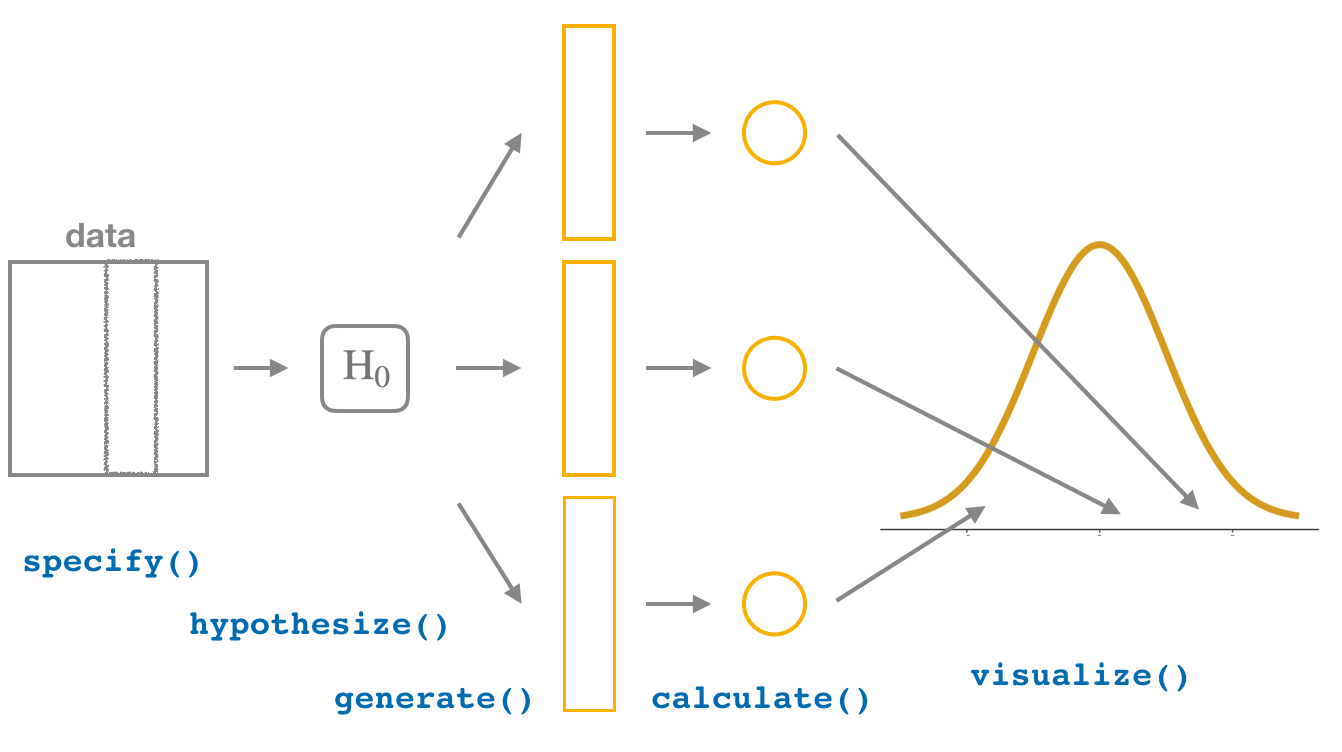
\includegraphics[width=0.7\linewidth,height=0.5\textheight]{week12_7} \end{center}
\end{frame}

\begin{frame}[fragile]{\texttt{infer} package workflow: \texttt{specify}
variables}
\protect\hypertarget{infer-package-workflow-specify-variables}{}
Recall that we use the \texttt{specify()} verb to specify the response
variable and, if needed, any explanatory variables for our study.

\tiny

\begin{Shaded}
\begin{Highlighting}[]
\NormalTok{promotions }\SpecialCharTok{\%\textgreater{}\%} 
  \FunctionTok{specify}\NormalTok{(}\AttributeTok{formula =}\NormalTok{ decision }\SpecialCharTok{\textasciitilde{}}\NormalTok{ gender, }\AttributeTok{success =} \StringTok{"promoted"}\NormalTok{)}
\end{Highlighting}
\end{Shaded}

\begin{verbatim}
Response: decision (factor)
Explanatory: gender (factor)
# A tibble: 48 x 2
   decision gender
   <fct>    <fct> 
 1 promoted male  
 2 promoted male  
 3 promoted male  
 4 promoted male  
 5 promoted male  
 6 promoted male  
 7 promoted male  
 8 promoted male  
 9 promoted male  
10 promoted male  
# i 38 more rows
\end{verbatim}

\normalsize
\end{frame}

\begin{frame}[fragile]{\texttt{infer} package workflow:
\texttt{hypothesize} the null}
\protect\hypertarget{infer-package-workflow-hypothesize-the-null}{}
In order to conduct hypothesis tests using the infer workflow, we need a
new step not present for confidence intervals: \texttt{hypothesize()}.

\[\begin{array}{ll}
&H_0: p_m-p_f=0\\
vs&H_A: p_m-p_f>0
\end{array}\]

\begin{itemize}
\item
  We set this null hypothesis \(H_0\) in our infer workflow using the
  null argument of the \texttt{hypothesize()} function to either:

  \begin{itemize}
  \tightlist
  \item
    ``point'' for hypotheses involving a single sample or
  \item
    ``independence'' for hypotheses involving two samples.
  \end{itemize}
\end{itemize}

Where do the terms ``\texttt{point}'' and ``\texttt{independence}'' come
from? These are two technical statistical terms.
\end{frame}

\begin{frame}{\texttt{infer} package workflow: \texttt{hypothesize} the
null}
\protect\hypertarget{infer-package-workflow-hypothesize-the-null-1}{}
\begin{itemize}
\item
  The term ``point'' relates from the fact that for a single group of
  observations, you will test the value of a single point.

  \begin{itemize}
  \tightlist
  \item
    Going back to the pennies example, say we wanted to test if the mean
    year of all US pennies was equal to 1993 or not.
  \item
    We would be testing the value of a ``point'' \(\mu\), the mean year
    of all US pennies, as follows:
  \end{itemize}
\end{itemize}

\[\begin{array}{ll}
&H_0: \mu=1993\\
vs&H_A: \mu\neq 1993
\end{array}\]
\end{frame}

\begin{frame}[fragile]{\texttt{infer} package workflow:
\texttt{hypothesize} the null}
\protect\hypertarget{infer-package-workflow-hypothesize-the-null-2}{}
\begin{itemize}
\item
  The term ``independence'' relates to the fact that for two groups of
  observations,

  \begin{itemize}
  \tightlist
  \item
    you are testing whether or not the response variable is independent
    of the explanatory variable that assigns the groups.
  \item
    In our case, we are testing whether the \texttt{decision} response
    variable is ``independent'' of the explanatory variable
    \texttt{gender} that assigns each résumé to either of the two
    groups.
  \end{itemize}
\end{itemize}
\end{frame}

\begin{frame}[fragile]{\texttt{infer} package workflow:
\texttt{hypothesize} the null}
\protect\hypertarget{infer-package-workflow-hypothesize-the-null-3}{}
\begin{Shaded}
\begin{Highlighting}[]
\NormalTok{promotions }\SpecialCharTok{\%\textgreater{}\%} 
  \FunctionTok{specify}\NormalTok{(}\AttributeTok{formula =}\NormalTok{ decision }\SpecialCharTok{\textasciitilde{}}\NormalTok{ gender, }
          \AttributeTok{success =} \StringTok{"promoted"}\NormalTok{) }\SpecialCharTok{\%\textgreater{}\%} 
  \FunctionTok{hypothesize}\NormalTok{(}\AttributeTok{null =} \StringTok{"independence"}\NormalTok{)}
\end{Highlighting}
\end{Shaded}
\end{frame}

\begin{frame}[fragile]{\texttt{infer} package workflow:
\texttt{generate} replicates}
\protect\hypertarget{infer-package-workflow-generate-replicates}{}
\begin{itemize}
\item
  After we \texttt{hypothesize()} the null hypothesis, we
  \texttt{generate()} replicates of ``shuffled'' datasets assuming the
  null hypothesis is true.

  \begin{itemize}
  \item
    For confidence intervals we generated replicates using
    \texttt{type\ =\ "bootstrap"}- resampling with \textbf{replacement}.
  \item
    For hypothesis testing we generate replicates using
    \texttt{type\ =\ "permute"} - resampling \textbf{without}
    replacement.
  \end{itemize}
\end{itemize}
\end{frame}

\begin{frame}[fragile]{\texttt{infer} package workflow:
\texttt{generate} replicates}
\protect\hypertarget{infer-package-workflow-generate-replicates-1}{}
\begin{Shaded}
\begin{Highlighting}[]
\NormalTok{promotions\_generate }\OtherTok{\textless{}{-}}\NormalTok{ promotions }\SpecialCharTok{\%\textgreater{}\%} 
  \FunctionTok{specify}\NormalTok{(}\AttributeTok{formula =}\NormalTok{ decision }\SpecialCharTok{\textasciitilde{}}\NormalTok{ gender, }
          \AttributeTok{success =} \StringTok{"promoted"}\NormalTok{) }\SpecialCharTok{\%\textgreater{}\%} 
  \FunctionTok{hypothesize}\NormalTok{(}\AttributeTok{null =} \StringTok{"independence"}\NormalTok{) }\SpecialCharTok{\%\textgreater{}\%} 
  \FunctionTok{generate}\NormalTok{(}\AttributeTok{reps =} \DecValTok{1000}\NormalTok{, }\AttributeTok{type =} \StringTok{"permute"}\NormalTok{)}
\end{Highlighting}
\end{Shaded}

Note: we performed shuffles/permutations for each of the 48 rows 1000
times and \(48,000=1000\cdot 48\).
\end{frame}

\begin{frame}[fragile]{\texttt{infer} package workflow:
\texttt{calculate} summary statistics}
\protect\hypertarget{infer-package-workflow-calculate-summary-statistics}{}
Now that we have generated 1000 replicates of ``shuffles'' assuming the
null hypothesis is true, let's \texttt{calculate()} the appropriate
summary statistic for each of our 1000 shuffles.

\begin{itemize}
\item
  the test statistic here is the difference in sample proportions
  \(\hat{p}_m-\hat{p}_f\).

  \begin{itemize}
  \tightlist
  \item
    we can calculate this test statistic by setting
    \texttt{stat\ =\ "diff\ in\ props"}.
  \item
    Furthermore, since we are interested in \(\hat{p}_m-\hat{p}_f\), we
    set \texttt{order\ =\ c("male",\ "female")}.
  \end{itemize}
\end{itemize}

Note: the order of the subtraction does not matter, so long as you stay
consistent throughout your analysis and tailor your interpretations
accordingly.
\end{frame}

\begin{frame}[fragile]{\texttt{infer} package workflow:
\texttt{calculate} summary statistics}
\protect\hypertarget{infer-package-workflow-calculate-summary-statistics-1}{}
\tiny

\begin{Shaded}
\begin{Highlighting}[]
\FunctionTok{set.seed}\NormalTok{(}\DecValTok{37}\NormalTok{)}
\NormalTok{promotions }\SpecialCharTok{\%\textgreater{}\%} 
  \FunctionTok{specify}\NormalTok{(}\AttributeTok{formula =}\NormalTok{ decision }\SpecialCharTok{\textasciitilde{}}\NormalTok{ gender, }\AttributeTok{success =} \StringTok{"promoted"}\NormalTok{) }\SpecialCharTok{\%\textgreater{}\%} 
  \FunctionTok{hypothesize}\NormalTok{(}\AttributeTok{null =} \StringTok{"independence"}\NormalTok{) }\SpecialCharTok{\%\textgreater{}\%} 
  \FunctionTok{generate}\NormalTok{(}\AttributeTok{reps =} \DecValTok{1000}\NormalTok{, }\AttributeTok{type =} \StringTok{"permute"}\NormalTok{) }\SpecialCharTok{\%\textgreater{}\%} 
  \FunctionTok{calculate}\NormalTok{(}\AttributeTok{stat =} \StringTok{"diff in props"}\NormalTok{, }\AttributeTok{order =} \FunctionTok{c}\NormalTok{(}\StringTok{"male"}\NormalTok{, }\StringTok{"female"}\NormalTok{)) }\OtherTok{{-}\textgreater{}}\NormalTok{ null\_distribution}
\NormalTok{null\_distribution}
\end{Highlighting}
\end{Shaded}

\begin{verbatim}
Response: decision (factor)
Explanatory: gender (factor)
Null Hypothesis: independence
# A tibble: 1,000 x 2
   replicate    stat
       <int>   <dbl>
 1         1 -0.125 
 2         2 -0.0417
 3         3 -0.0417
 4         4 -0.0417
 5         5 -0.125 
 6         6  0.125 
 7         7  0.125 
 8         8 -0.125 
 9         9  0.125 
10        10 -0.292 
# i 990 more rows
\end{verbatim}

\normalsize
\end{frame}

\begin{frame}[fragile]{\texttt{infer} package workflow:
\texttt{calculate} summary statistics}
\protect\hypertarget{infer-package-workflow-calculate-summary-statistics-2}{}
What was the observed difference in promotion rates?

\begin{Shaded}
\begin{Highlighting}[]
\NormalTok{obs\_diff\_prop }\OtherTok{\textless{}{-}}\NormalTok{ promotions }\SpecialCharTok{\%\textgreater{}\%} 
  \FunctionTok{specify}\NormalTok{(decision }\SpecialCharTok{\textasciitilde{}}\NormalTok{ gender, }\AttributeTok{success =} \StringTok{"promoted"}\NormalTok{) }\SpecialCharTok{\%\textgreater{}\%} 
  \FunctionTok{calculate}\NormalTok{(}\AttributeTok{stat =} \StringTok{"diff in props"}\NormalTok{, }
            \AttributeTok{order =} \FunctionTok{c}\NormalTok{(}\StringTok{"male"}\NormalTok{, }\StringTok{"female"}\NormalTok{))}
\NormalTok{obs\_diff\_prop}
\end{Highlighting}
\end{Shaded}

\begin{verbatim}
Response: decision (factor)
Explanatory: gender (factor)
# A tibble: 1 x 1
   stat
  <dbl>
1 0.292
\end{verbatim}
\end{frame}

\begin{frame}[fragile]{\texttt{infer} package workflow:
\texttt{visualize} the p-value}
\protect\hypertarget{infer-package-workflow-visualize-the-p-value}{}
The final step is to measure how surprised we are by a promotion
difference of \(29.2\%\) in a hypothesized universe of no gender
discrimination

\begin{itemize}
\tightlist
\item
  Furthermore, we'll set the direction = ``right'' reflecting our
  alternative hypothesis \(H_A: p_m-p_f>0\). Set
  \texttt{direction\ =\ "both"} for two-sided \(H_A: p_m-p_f\neq 0\).
\end{itemize}

\tiny

\begin{Shaded}
\begin{Highlighting}[]
\FunctionTok{visualize}\NormalTok{(null\_distribution, }\AttributeTok{bins =} \DecValTok{10}\NormalTok{) }\SpecialCharTok{+} 
  \FunctionTok{shade\_p\_value}\NormalTok{(}\AttributeTok{obs\_stat =}\NormalTok{ obs\_diff\_prop, }\AttributeTok{direction =} \StringTok{"right"}\NormalTok{) }\SpecialCharTok{+} 
  \FunctionTok{theme\_bw}\NormalTok{()}
\end{Highlighting}
\end{Shaded}

\begin{center}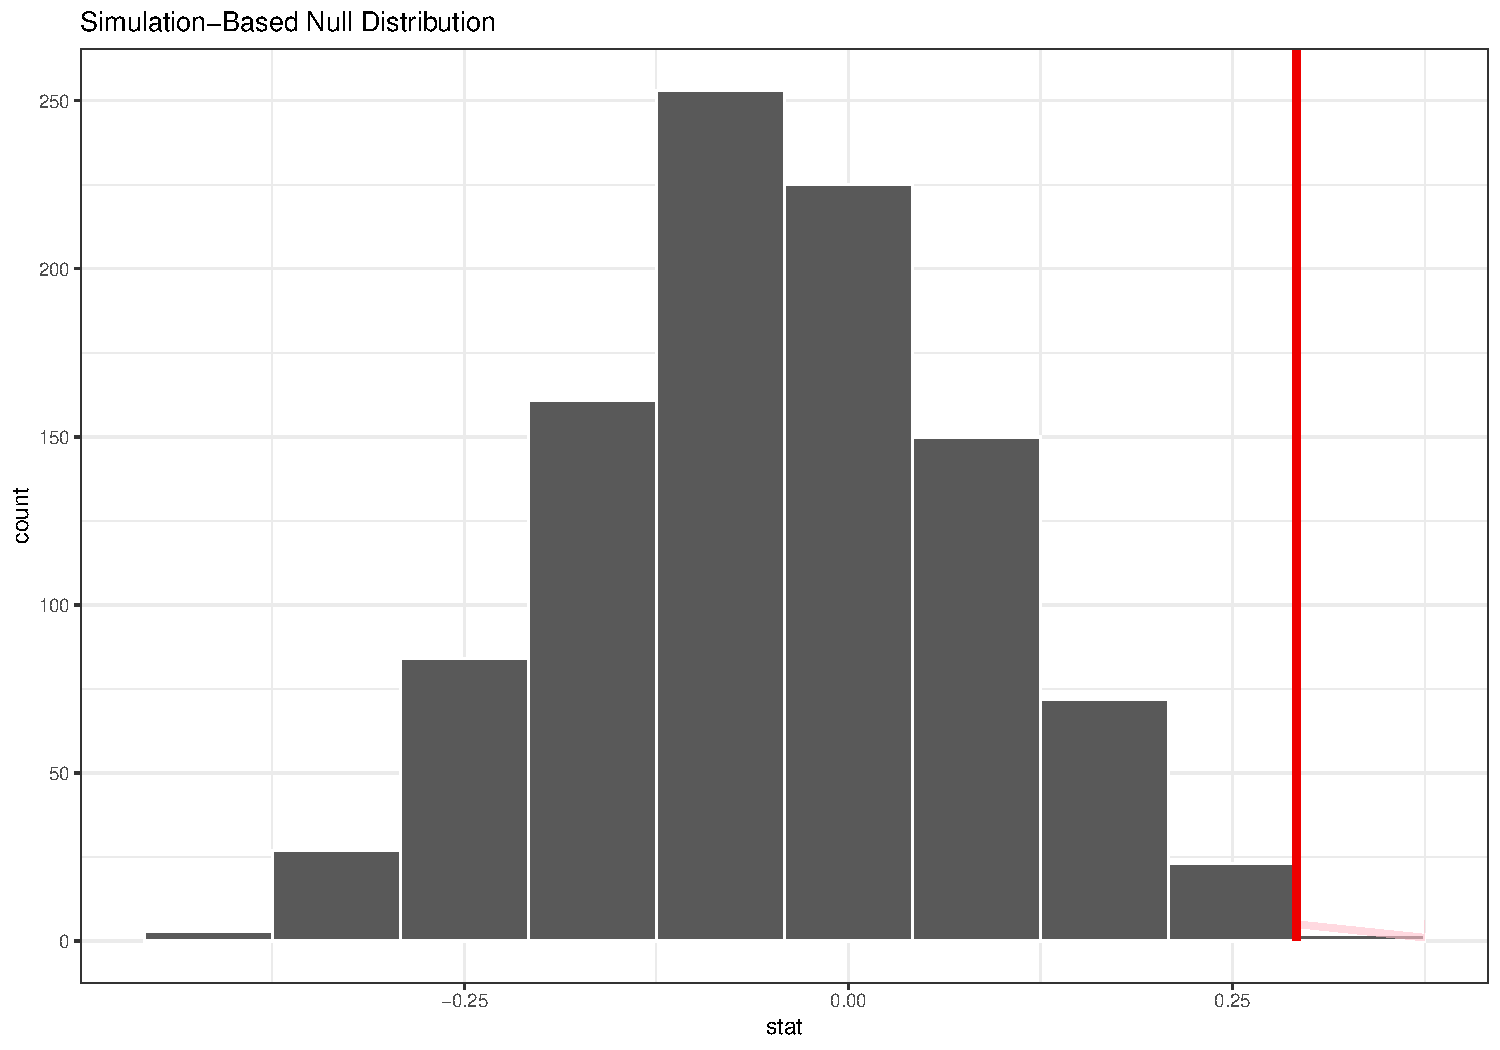
\includegraphics[width=0.7\linewidth,height=0.4\textheight]{Week11_12_13_files/figure-beamer/unnamed-chunk-55-1} \end{center}
\normalsize
\end{frame}

\begin{frame}[fragile]{\texttt{infer} package workflow:
\texttt{visualize} the p-value}
\protect\hypertarget{infer-package-workflow-visualize-the-p-value-1}{}
\begin{itemize}
\item
  However, what does the shaded-region correspond to? This is the
  \textbf{p-value}.

  \begin{itemize}
  \tightlist
  \item
    A p-value is the probability of obtaining a test statistic just as
    or more extreme than the observed test statistic assuming the null
    hypothesis \(H_0\) is true.
  \end{itemize}
\item
  So judging by the shaded region in the figure, it seems we would
  somewhat rarely observe differences in promotion rates of
  \(0.292 = 29.2\%\) or more in a hypothesized universe of no gender
  discrimination.
\end{itemize}

\tiny

\begin{Shaded}
\begin{Highlighting}[]
\NormalTok{null\_distribution }\SpecialCharTok{\%\textgreater{}\%} 
  \FunctionTok{get\_p\_value}\NormalTok{(}\AttributeTok{obs\_stat =} \FloatTok{0.292}\NormalTok{, }\AttributeTok{direction =} \StringTok{"right"}\NormalTok{) }
\end{Highlighting}
\end{Shaded}

\begin{verbatim}
# A tibble: 1 x 1
  p_value
    <dbl>
1   0.002
\end{verbatim}

\begin{Shaded}
\begin{Highlighting}[]
\CommentTok{\# Or}
\FunctionTok{mean}\NormalTok{(null\_distribution}\SpecialCharTok{$}\NormalTok{stat }\SpecialCharTok{\textgreater{}=} \FloatTok{0.292}\NormalTok{)}
\end{Highlighting}
\end{Shaded}

\begin{verbatim}
[1] 0.002
\end{verbatim}

\normalsize
\end{frame}

\begin{frame}{\texttt{infer} package workflow: \texttt{visualize} the
p-value}
\protect\hypertarget{infer-package-workflow-visualize-the-p-value-2}{}
Since this p-value is smaller than our pre-specified significance level
\(\alpha=0.05\), we reject the null hypothesis \(H_0: p_m-p_f=0\).

\begin{itemize}
\item
  In other words, this p-value is sufficiently small to reject our
  hypothesized universe of no gender discrimination.
\item
  We instead have enough evidence to change our mind in favor of gender
  discrimination being a likely culprit here.
\end{itemize}
\end{frame}

\begin{frame}[fragile]{Comparison with confidence intervals}
\protect\hypertarget{comparison-with-confidence-intervals}{}
This is the entire code that creates the null distribution.

\begin{Shaded}
\begin{Highlighting}[]
\FunctionTok{set.seed}\NormalTok{(}\DecValTok{37}\NormalTok{)}
\NormalTok{null\_distribution }\OtherTok{\textless{}{-}}\NormalTok{ promotions }\SpecialCharTok{\%\textgreater{}\%} 
  \FunctionTok{specify}\NormalTok{(}\AttributeTok{formula =}\NormalTok{ decision }\SpecialCharTok{\textasciitilde{}}\NormalTok{ gender, }
          \AttributeTok{success =} \StringTok{"promoted"}\NormalTok{) }\SpecialCharTok{\%\textgreater{}\%} 
  \FunctionTok{hypothesize}\NormalTok{(}\AttributeTok{null =} \StringTok{"independence"}\NormalTok{) }\SpecialCharTok{\%\textgreater{}\%} 
  \FunctionTok{generate}\NormalTok{(}\AttributeTok{reps =} \DecValTok{1000}\NormalTok{, }\AttributeTok{type =} \StringTok{"permute"}\NormalTok{) }\SpecialCharTok{\%\textgreater{}\%} 
  \FunctionTok{calculate}\NormalTok{(}\AttributeTok{stat =} \StringTok{"diff in props"}\NormalTok{, }
            \AttributeTok{order =} \FunctionTok{c}\NormalTok{(}\StringTok{"male"}\NormalTok{, }\StringTok{"female"}\NormalTok{))}
\end{Highlighting}
\end{Shaded}
\end{frame}

\begin{frame}[fragile]{Comparison with confidence intervals}
\protect\hypertarget{comparison-with-confidence-intervals-1}{}
We need to make \textbf{two changes two changes} to create the bootstrap
distribution needed to construct a \(95\%\) confidence interval for
\(p_m-p_f\).

\begin{Shaded}
\begin{Highlighting}[]
\NormalTok{bootstrap\_distribution }\OtherTok{\textless{}{-}}\NormalTok{ promotions }\SpecialCharTok{\%\textgreater{}\%} 
  \FunctionTok{specify}\NormalTok{(}\AttributeTok{formula =}\NormalTok{ decision }\SpecialCharTok{\textasciitilde{}}\NormalTok{ gender, }
          \AttributeTok{success =} \StringTok{"promoted"}\NormalTok{) }\SpecialCharTok{\%\textgreater{}\%} 
  \CommentTok{\# Change 1 {-} Remove hypothesize():}
  \CommentTok{\# hypothesize(null = "independence") \%\textgreater{}\% }
  \CommentTok{\# Change 2 {-} Switch type from "permute" to "bootstrap":}
  \FunctionTok{generate}\NormalTok{(}\AttributeTok{reps =} \DecValTok{1000}\NormalTok{, }\AttributeTok{type =} \StringTok{"bootstrap"}\NormalTok{) }\SpecialCharTok{\%\textgreater{}\%} 
  \FunctionTok{calculate}\NormalTok{(}\AttributeTok{stat =} \StringTok{"diff in props"}\NormalTok{, }
            \AttributeTok{order =} \FunctionTok{c}\NormalTok{(}\StringTok{"male"}\NormalTok{, }\StringTok{"female"}\NormalTok{))}
\end{Highlighting}
\end{Shaded}
\end{frame}

\begin{frame}[fragile]{Comparison with confidence intervals}
\protect\hypertarget{comparison-with-confidence-intervals-2}{}
\tiny

\begin{Shaded}
\begin{Highlighting}[]
\NormalTok{percentile\_ci }\OtherTok{\textless{}{-}}\NormalTok{ bootstrap\_distribution }\SpecialCharTok{\%\textgreater{}\%} 
  \FunctionTok{get\_confidence\_interval}\NormalTok{(}\AttributeTok{level =} \FloatTok{0.95}\NormalTok{, }\AttributeTok{type =} \StringTok{"percentile"}\NormalTok{)}
\NormalTok{percentile\_ci}
\end{Highlighting}
\end{Shaded}

\begin{verbatim}
# A tibble: 1 x 2
  lower_ci upper_ci
     <dbl>    <dbl>
1   0.0414    0.535
\end{verbatim}

\begin{Shaded}
\begin{Highlighting}[]
\FunctionTok{visualize}\NormalTok{(bootstrap\_distribution) }\SpecialCharTok{+} 
  \FunctionTok{shade\_confidence\_interval}\NormalTok{(}\AttributeTok{endpoints =}\NormalTok{ percentile\_ci) }\SpecialCharTok{+} 
  \FunctionTok{theme\_bw}\NormalTok{()}
\end{Highlighting}
\end{Shaded}

\begin{center}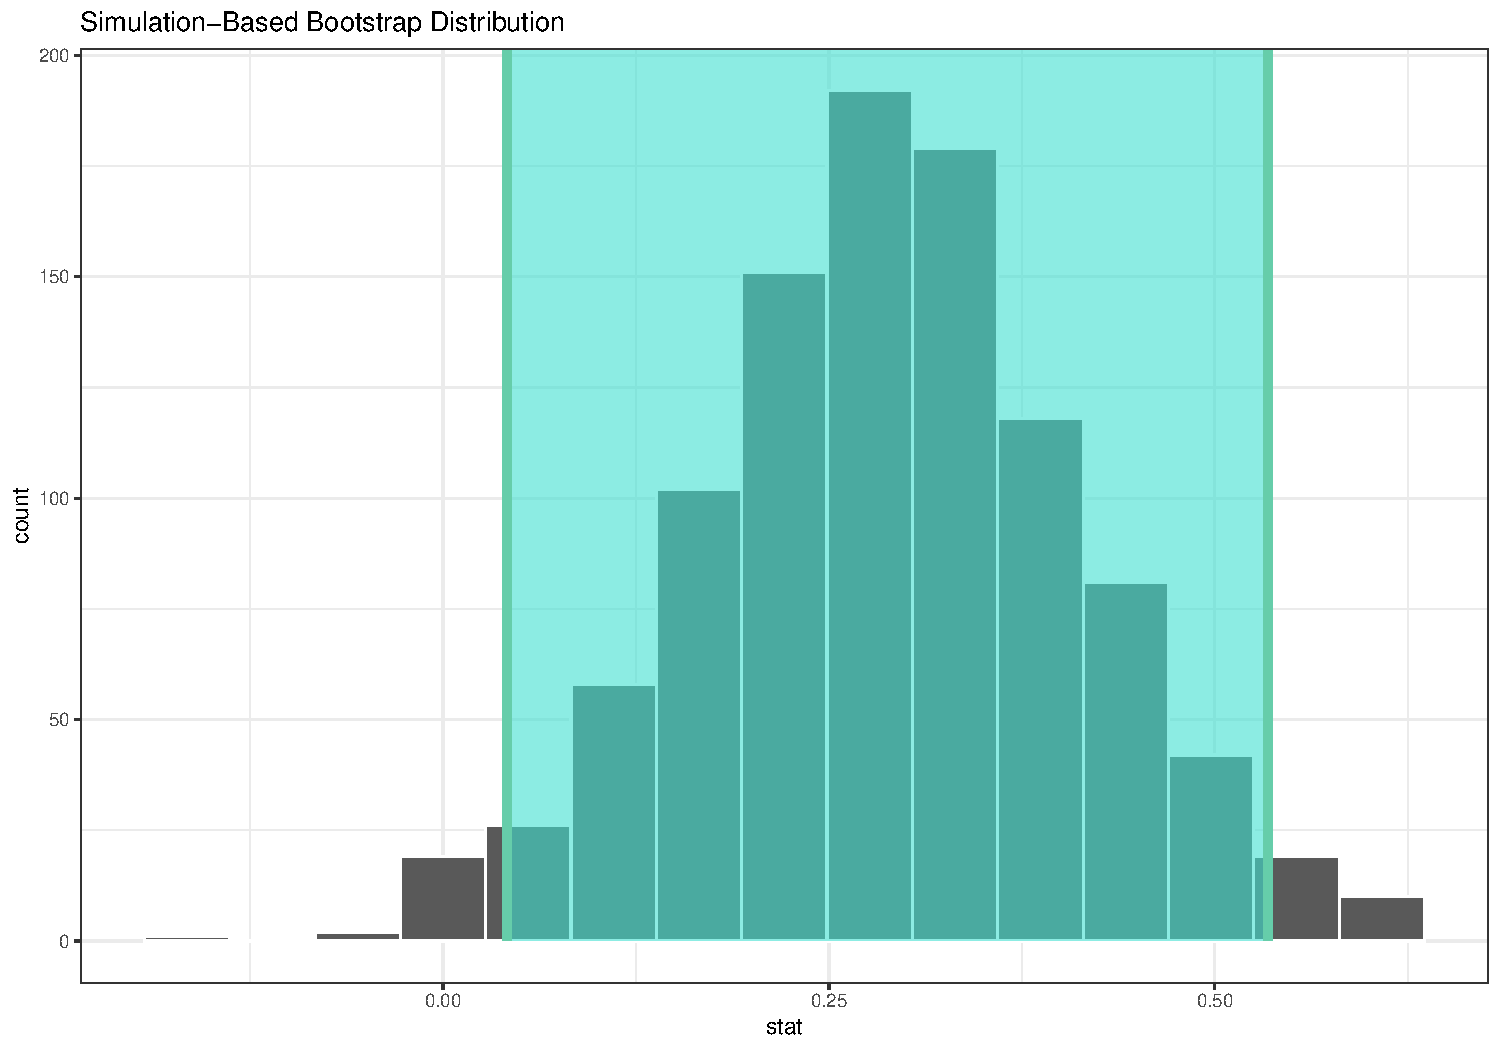
\includegraphics[width=0.7\linewidth,height=0.35\textheight]{Week11_12_13_files/figure-beamer/unnamed-chunk-59-1} \end{center}
\normalsize

Notice how the value 0 is not included in our confidence interval, again
suggesting that \(p_m\) and \(p_f\) are truly different!
\end{frame}

\begin{frame}{Summary}
\protect\hypertarget{summary}{}
\begin{itemize}
\item
  If you can understand the framework, you can easily generalize these
  ideas for all hypothesis testing scenarios. Whether for:

  \begin{itemize}
  \tightlist
  \item
    population proportions \(p\)
  \item
    population means \(\mu\)
  \item
    differences in population proportions \(p_1-p_2\)
  \item
    differences in population means \(\mu_1-\mu_2\)
  \end{itemize}
\end{itemize}

\begin{center}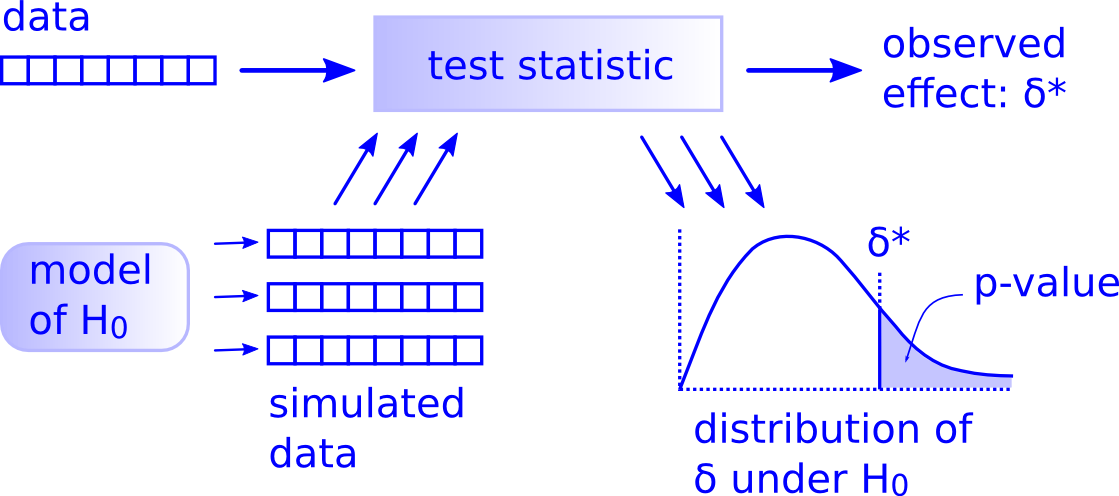
\includegraphics[width=0.7\linewidth,height=0.5\textheight]{week12_8} \end{center}
\end{frame}

\hypertarget{interpreting-hypothesis-tests}{%
\section{Interpreting hypothesis
tests}\label{interpreting-hypothesis-tests}}

\begin{frame}{Interpreting hypothesis tests}
\protect\hypertarget{interpreting-hypothesis-tests-1}{}
\begin{itemize}
\item
  We mentioned that given a pre-specified significance level \(\alpha\)
  there are two possible outcomes of a hypothesis test:

  \begin{itemize}
  \tightlist
  \item
    If the p-value is less than \(\alpha\) then we \textbf{reject} the
    null hypothesis \(H_0\) in favor of \(H_A\).
  \item
    If the p-value is greater than \(\alpha\) then we \textbf{fail to
    reject} the null hypothesis \(H_0\).
  \end{itemize}
\item
  Unfortunately, the latter result is often misinterpreted as
  ``accepting the null hypothesis \(H_0\).

  \begin{itemize}
  \tightlist
  \item
    Saying that we ``accept the null hypothesis \(H_0\)'' is equivalent
    to stating that ``we think the null hypothesis \(H_0\) is true.
  \item
    Saying that we ``fail to reject the null hypothesis \(H_0\)'' is
    saying something else: ``While \(H_0\) might still be false, we
    don't have enough evidence to say so.''
  \end{itemize}
\end{itemize}
\end{frame}

\begin{frame}{Interpreting hypothesis tests}
\protect\hypertarget{interpreting-hypothesis-tests-2}{}
Let's use the United States criminal justice system as an analogy.

\begin{itemize}
\item
  A criminal trial in the United States is a similar situation to
  hypothesis tests whereby a choice between two contradictory claims
  must be made about a defendant who is on trial:

  \begin{itemize}
  \tightlist
  \item
    The defendant is truly either ``innocent'' (\(H_0\)) or
    ``guilty.''(\(H_A\))
  \item
    The defendant is presumed ``innocent until proven guilty.''
  \item
    The defendant is found guilty only if there is strong evidence that
    the defendant is guilty. The phrase ``beyond a reasonable doubt''
    (significance level \(\alpha\)) is often used as a guideline for
    determining a cutoff for when enough evidence exists to find the
    defendant guilty.
  \item
    The defendant is found to be either ``not guilty''(fail to reject
    \(H_0\)) or ``guilty'' in the ultimate verdict.
  \end{itemize}
\item
  In other words, not guilty verdicts are not suggesting the defendant
  is innocent.
\end{itemize}
\end{frame}

\begin{frame}{Types of errors}
\protect\hypertarget{types-of-errors}{}
\begin{itemize}
\item
  Nobody's perfect. Even with lots of evidence, we can still make wrong
  decisions.
\item
  In fact, when we perform a hypothesis test, we can make mistakes in
  two ways:

  \begin{itemize}
  \tightlist
  \item
    \textbf{Type I Error}: The null hypothesis is true, but we
    miskakenly reject it.
  \item
    \textbf{Type II Error}: The null hypothesis is false, but we fail to
    reject it.
  \end{itemize}
\item
  One way to keep the names straight is to remember that we start by
  assuming the null hypothesis is true, so \textbf{Type I error} is the
  first kind of error we could make.
\end{itemize}
\end{frame}

\begin{frame}{Types of errors}
\protect\hypertarget{types-of-errors-1}{}
The Type I and II errors can be illustrated in the Table of TRUTH below:

\begin{center}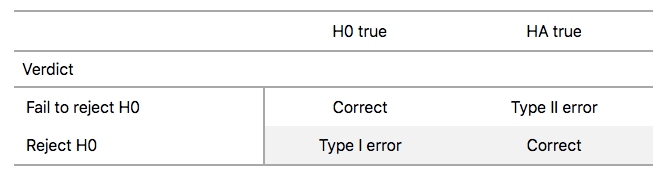
\includegraphics[width=0.6\linewidth,height=0.3\textheight]{week12_9a} \end{center}

We apply these terms to our criminal justice analogy

\begin{center}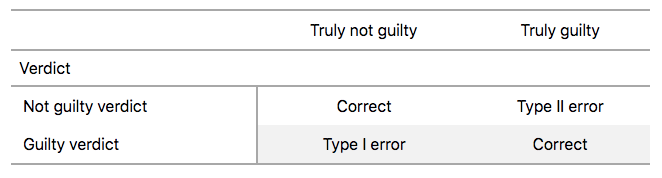
\includegraphics[width=0.6\linewidth,height=0.3\textheight]{week12_9b} \end{center}
\end{frame}

\begin{frame}{Probabilities of Type I and II Errors}
\protect\hypertarget{probabilities-of-type-i-and-ii-errors}{}
\begin{itemize}
\item
  \(P(\text{Type I Error})=P(\text{Reject } H_0 | H_0 \text{ true})=\alpha\)

  \begin{itemize}
  \tightlist
  \item
    This represents the probability that if \(H_0\) is true then we will
    reject \(H_0\).
  \item
    Type I error occurs when the null hypothesis is true but we've had
    the bad luck to draw an unusual sample.
  \item
    If you have a small p-value, you could make this error. Because
    P-value \(\leq \alpha \implies\) Reject \(H_0\)
  \end{itemize}
\item
  \(P(\text{Type II Error})=P(\text{Fail to reject } H_0 | H_0 \text{ false})=\beta\)

  \begin{itemize}
  \tightlist
  \item
    The probability of failing to reject a false null hypothesis is a
    Type II error.
  \item
    Harder to calculate \(\beta\). This is because when \(H_0\) is
    false, we don't know the parameter value and there are many possible
    values.
  \item
    If you have a large p-value, you could make this error.
  \item
    The value \(1-\beta\) is known as the \textbf{power} of the
    hypothesis test.
  \end{itemize}
\end{itemize}
\end{frame}

\begin{frame}{Relationship Between Sample Size, Errors, and Power}
\protect\hypertarget{relationship-between-sample-size-errors-and-power}{}
\begin{columns}
\begin{column}{0.3\textwidth}
Below we test: 
$$H_0:p=p_0 $$
$$ \text{vs.} $$
$$H_A:p>p_o $$
\end{column}
\begin{column}{0.5\textwidth}


\begin{center}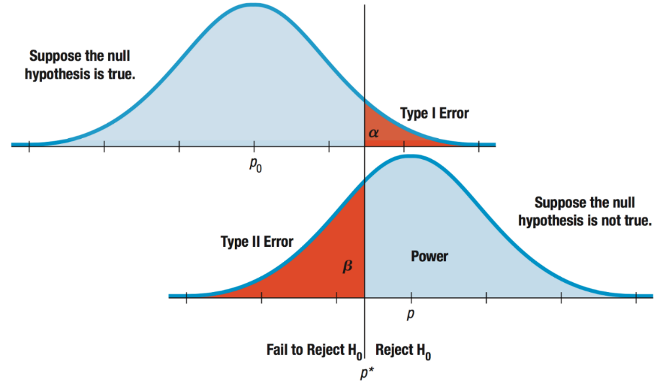
\includegraphics[width=1\linewidth]{week13_2} \end{center}

\end{column}
\end{columns}

\begin{itemize}
\item
  The top figure, \(p_0\) is the true proportion.

  \begin{itemize}
  \tightlist
  \item
    A high \(\hat{p}\) results in a Type I error.
  \end{itemize}
\item
  The bottom figure, \(p\) is the true proportion with a distribution of
  possible observed \(\hat{p}\) values around this true value.

  \begin{itemize}
  \item
    Because of this sampling variability, sometimes \(\hat{p} < p*\) and
    we fail to reject the false null hypothesis
  \item
    A low \(\hat{p}\) near \(p_0\) results in a Type II error.
  \end{itemize}
\end{itemize}
\end{frame}

\begin{frame}{Relationship Between Errors, and Power}
\protect\hypertarget{relationship-between-errors-and-power}{}
\begin{itemize}
\item
  Decreasing \(\alpha\) results in an increase of \(\beta\) (reduce
  power).
\item
  What is typically done in practice is to fix the probability of a Type
  I error by pre-specifying a significance level \(\alpha\) and then try
  to minimize \(\beta\).
\item
  For a given \(\alpha\) level, to reduce \(\beta\) (increase power),
  one MUST increase sample size!

  \begin{itemize}
  \tightlist
  \item
    SD goes down.
  \item
    \(\beta\) goes down and power increases.
  \end{itemize}
\end{itemize}

\begin{columns}
\begin{column}{0.3\textwidth}



\begin{center}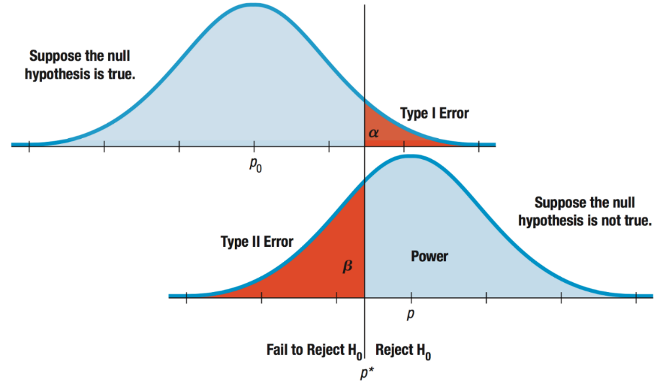
\includegraphics[width=1\linewidth]{week13_2} \end{center}


\end{column}
\begin{column}{0.3\textwidth}


\begin{center}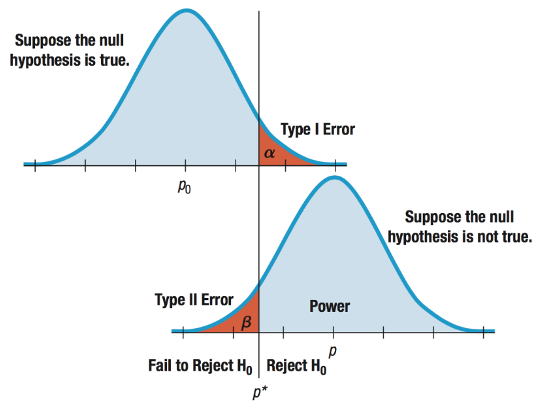
\includegraphics[width=1\linewidth]{week13_3} \end{center}

\end{column}
\end{columns}
\end{frame}

\end{document}
